\documentclass[twoside,nogutter]{glasgowthesis}
%\documentclass[twoside,hidelinks]{glasgowthesis}
% ^^ draft shows overfilled boxes (but disables links)
% ^^ replace "oneside" with "twoside" to set the gutter correctly for
%    two-sided printing.
% ^^ add "nogutter" option for digital copy (without binding offsets),
%    if printed copy is twoside, use [twoside,nogutter] for digital copy.
% ^^ add "hidelinks" option to remove coloured links (e.g. for printing)

%%%
% Packages

\usepackage{graphicx}
\usepackage{amsmath}
\usepackage{amssymb}
\usepackage{color}
\usepackage{bookmark}
\usepackage{hyphenat} % for \hyp{} instead of "-".

%%%
% Bibliography

% import package and set some options
\usepackage[minnames=1,maxnames=5,style=numeric-comp,sorting=none,url=false,backend=bibtex]{biblatex}

% set path to database
\bibliography{bibliography.bib}

%%%
% SI units

% import package, with astronomy units
\usepackage[separate-uncertainty=true,alsoload=astro]{siunitx}

% for nice display of negative symbol in equations
\sisetup{
   detect-mode,
   detect-family,
   detect-inline-family=math,
   detect-weight=true
}

% sqrt(Hz)
\DeclareSIUnit{\sqrthz}{\ensuremath{\sqrt{\textrm{\hertz}}}}

% ppm
\DeclareSIUnit{\ppm}{\ensuremath{\textrm{ppm}}}

%%%
% List of symbols, definitions, etc.

% import package
\usepackage[acronym,nomain]{glossaries}

% make the list
\makeglossaries

%%%
% superscript th, st, nd, rd, etc.
\usepackage[super]{nth}

%%%
% Fix silly LaTeX space/punctuation behaviour with custom commands
%
% The command '\xspace' should be added to the end of custom commands which lack arguments, to make LaTeX put a space after the command's output.
\usepackage{xspace}

%%%
% Smaller text in captions
\usepackage[font=small]{caption}

%%%
% Subcaptions
\usepackage{subcaption}

%%%
% Wrapping text around figures and tables
\usepackage{wrapfig}

%%%
% Sideways figures
\usepackage{rotating}

%%%
% Formatting of ordinal numbers, i.e. 1st, 2nd, 3rd, as superscripts
\usepackage[super]{nth}

%%%
% Chemical symbols
\usepackage[version=3]{mhchem}

%%%
% Code listings
% https://www.ctan.org/tex-archive/macros/latex/contrib/listings/
\usepackage{listings}

%%%
% Hyperlinks
%
% (This should be as close to the end of the package imports as possible - see https://www.tug.org/applications/hyperref/manual.html)

% import package
\usepackage{hyperref}
\hypersetup{
  colorlinks=true,
  linkcolor=blue,
  filecolor=magenta,      
  urlcolor=cyan
}

%%%
% Custom commands

% command to make plural versions of commands (http://tex.stackexchange.com/questions/259287/how-to-define-a-newcommand-that-expands-into-another-newcommand)
% e.g.
% 	\makename[es]{veggie}{potato}
% makes the commands \veggie (=potato) and \veggies (=potatoes)
\newcommand{\makename}[3][s]{%
  \expandafter\newcommand\csname #2\endcsname{#3\xspace}%
  \expandafter\newcommand\csname #2s\endcsname{#3#1\xspace}%
}

% red, italic, bold - for notes
\newcommand{\note}[1]{\textcolor{red}{\emph{[\textbf{Note: }#1]}}}

% blue, normal text - for statements that need fact-checked
\newcommand{\checkme}[1]{\textcolor{blue}{#1}}

% naive with diaeresis
\newcommand{\naive}{na\"ive\xspace}

% et al.
% (and a backslash to prevent TeX thinking a new sentence starts afterwards)
\newcommand{\etal}{et~al.\@}

% gravitational wave events
\newcommand{\GWFIRSTEVENT}{\gls{GW}150914}
\newcommand{\GWSECONDEVENT}{\gls{GW}151226}

% gravitational wave detectors
\newcommand{\GEO}{GEO 600}
\newcommand{\GEOHF}{GEO \gls{HF}}
\newcommand{\LIGO}{\gls{LIGO}}
\newcommand{\LLO}{\LIGO{} Livingston}
\newcommand{\LHO}{\LIGO{} Hanford}
\newcommand{\ILIGO}{Initial \LIGO{}}
\newcommand{\ALIGO}{Advanced \LIGO{}}
\newcommand{\INDIGO}{\gls{LIGO} India}
\newcommand{\LIGOVOYAGER}{\gls{LIGO} Voyager}
\newcommand{\LIGOCE}{\gls{LIGO} Cosmic Explorer}
\newcommand{\VIRGO}{Virgo}
\newcommand{\IVIRGO}{Initial \VIRGO{}}
\newcommand{\AVIRGO}{Advanced \VIRGO{}}
\newcommand{\KAGRA}{\gls{KAGRA}}
\newcommand{\ET}{Einstein Telescope}
\newcommand{\ETLF}{\gls{ET}-\gls{LF}}
\newcommand{\ETHF}{\gls{ET}-\gls{HF}}
\newcommand{\ELISA}{\gls{ELISA}}

% Michelson interferometer
\newcommand{\MI}{Michelson interferometer\xspace}

% Fabry-Perot with accent
\newcommand{\FP}{Fabry-Perot\xspace}

% Fabry-Perot Michelson interferometer
\newcommand{\FPMI}{\FP{} \MI{}\xspace}

% Power recycled Fabry-Perot Michelson interferometer
\newcommand{\PRFPMI}{power-recycled \FPMI{}\xspace}

% Dual-recycled Fabry-Perot Michelson interferometer
\newcommand{\DRFPMI}{dual-recycled \FPMI{}\xspace}

% speedmeter
\newcommand{\SM}{speed meter\xspace}

% Sagnac Speedmeter
\newcommand{\SSM}{Sagnac \SM{}\xspace}

% Sagnac Speedmeter experiment
\newcommand{\SSMEXPT}{\SSM{} experiment\xspace}

% AEI 10m prototype
\newcommand{\AEIPROTOTYPE}{AEI \SI{10}{\meter} prototype\xspace}

% Glasgow 10m prototype
\newcommand{\GLASGOWTENM}{Glasgow \SI{10}{\meter} prototype\xspace}

% Caltech 40m prototype
\newcommand{\CALTECHFORTYM}{Caltech \SI{40}{\meter} prototype\xspace}

% Garching
\newcommand{\GARCHINGPROTOTYPE}{Garching prototype\xspace}

% LIGO Scientific Collaboration
\newcommand{\LSC}{\gls{LIGO} Scientific Collaboration\xspace}

% Matlab
\newcommand{\MATLAB}{Matlab\xspace}
\newcommand{\SIMULINK}{\MATLAB Simulink\xspace}

% L minus
\newcommand{\LMINUS}{$L_{\left(-\right)}$}

% L plus
\newcommand{\LPLUS}{$L_{\left(+\right)}$}

% Scultety
\newcommand{\SCULTETY}{Scult\'{e}ty}

% Mirror names for Chapters 4 and 5
\newcommand{\MONEA}{$\textrm{M}_{\textrm{1}}^{\textrm{A}}$}
\newcommand{\MONEB}{$\textrm{M}_{\textrm{1}}^{\textrm{B}}$}
\newcommand{\MTWOA}{$\textrm{M}_{\textrm{2}}^{\textrm{A}}$}
\newcommand{\MTWOB}{$\textrm{M}_{\textrm{2}}^{\textrm{B}}$}
\newcommand{\MTHREEA}{$\textrm{M}_{\textrm{3}}^{\textrm{A}}$}
\newcommand{\MTHREEB}{$\textrm{M}_{\textrm{3}}^{\textrm{B}}$}
\newcommand{\MFOUR}{$\textrm{M}_{\textrm{4}}$}
\newcommand{\MFIVE}{$\textrm{M}_{\textrm{5}}$}
\newcommand{\MSIX}{$\textrm{M}_{\textrm{6}}$}
\newcommand{\MSEVEN}{$\textrm{M}_{\textrm{7}}$}
\newcommand{\MEIGHT}{$\textrm{M}_{\textrm{8}}$}
\newcommand{\MNINE}{$\textrm{M}_{\textrm{9}}$}
\newcommand{\MTEN}{$\textrm{M}_{\textrm{10}}$}
\newcommand{\MELEVEN}{$\textrm{M}_{\textrm{11}}$}
\newcommand{\MTWELVE}{$\textrm{M}_{\textrm{12}}$}
\newcommand{\MTHIRTEEN}{$\textrm{M}_{\textrm{13}}$}
\newcommand{\MFOURTEEN}{$\textrm{M}_{\textrm{14}}$}
\newcommand{\MFIFTEEN}{$\textrm{M}_{\textrm{15}}$}
\newcommand{\MSIXTEEN}{$\textrm{M}_{\textrm{16}}$}

% Beam splitters etc. for Chapters 4 and 5
\newcommand{\HDA}{$\textrm{HD}_{\textrm{A}}$}
\newcommand{\HDB}{$\textrm{HD}_{\textrm{B}}$}

% title, contents, etc.
\frontmatter
%%%
% Document

\begin{document}

%\pagestyle{empty}
%\pagenumbering{gobble}

\title{Enhancing the Sensitivity of Future Laser-Interferometric Gravitational Wave Detectors}
\author{Sean Stephan Leavey}
\date{Month Year}

\maketitle

\cleardoublepage

%\pagenumbering{roman}
%\setcounter{page}{1}

% import glossary terms
\input{"00-definitions.tex"} 

\newpage

% ensures that the front matter appears in the PDF table of contents
\phantomsection

\input{"00-abstract.tex"}
\addcontentsline{toc}{section}{Abstract}

\newpage

\vspace*{2.75in}
\noindent Content from this work may be used under the terms of the \href{https://creativecommons.org/licenses/by-nc-sa/4.0/}{Creative Commons \emph{Attribution-NonCommercial-ShareAlike 4.0 International}} licence.

\begin{center}
  
\includegraphics[width=2in]{graphics/generated/from-svg/00-cc-by-nc-sa.pdf}
\end{center}
\addcontentsline{toc}{section}{Licence}

\newpage

% change contents title to lower case
\renewcommand{\contentsname}{Table of contents}
\tableofcontents
\addcontentsline{toc}{section}{Table of contents}

\listoftables
\addcontentsline{toc}{section}{List of tables}

\listoffigures
\addcontentsline{toc}{section}{List of figures}

\cleardoublepage
\section*{\label{c:intro:credits}Credits}
\input{"00-credits.tex"}
\addcontentsline{toc}{section}{Credits}

\cleardoublepage
\vspace*{1.75in}
\begin{flushright} Dedication.\end{flushright}
\addcontentsline{toc}{section}{Dedication}

% Number chapter boomarks
\bookmarksetup{numbered}

% main chapters
\mainmatter
\chapter{\label{c:gw-detection}Gravitational waves}

\section{Event GW150914}
One billion years ago a pair of black holes, one with \num{36} solar masses and the other with \num{29} solar masses, merged into a single black hole with \num{62} solar masses. The missing energy equivalent to \num{3} solar masses was radiated away in the form of gravitational waves.

At 09:50:45 \gls{UTC} on \nth{14} September 2015, gravitational waves from the event passed through the \LIGO{} Livingston detector, perturbing the mirrors by \SI{e-18}{\meter} and creating a signal large enough for the electronics controlling the interferometer to detect the ripple in space time more than \num{23} times above the background noise. Seven milliseconds later, the same wavefront passed the \LIGO{} Hanford detector and moved the mirrors in the opposite direction. At that moment, for the first time in human history, a gravitational wave had been detected.

From the gravitational waveform witnessed at the \LIGO{} sites it was possible to determine the type and parameters of the waves' source. The waveforms for \emph{\GWFIRSTEVENT{}}, as it became known, are consistent with a binary black hole merger where they are swept up in frequency before creating a loud ``chirp'' signal as shown in Figure\,\ref{fig:gw150914}. The signal was only above each detector's background noise for the last few \SI{}{\milli\second} of this process. Not only did \LIGO{} make the first observation of a gravitational wave, it also made the first detection of a binary black hole system and found the missing experimental proof of Einstein's theory of general relativity. The window into the universe opening up due to \LIGO{} and the worldwide network of gravitational wave detectors in operation and under assembly, \GEO{}, \VIRGO{} and \KAGRA{}, represents an opportunity to study the universe in a completely new way. Some secrets have already been discovered, but there are surely more to be uncovered.

\begin{figure}
  \centering
  \includegraphics[width=\columnwidth]{graphics/generated/from-python/10-gw150914.pdf}
  \caption[Measured strain from the LIGO Hanford and Livingston detectors around the time of event \GWFIRSTEVENT{}]{\label{fig:gw150914}Measured strain from the \LIGO{} Hanford and Livingston detectors around the time of event \GWFIRSTEVENT{}, the first recorded gravitational wave in history. Once a promising signal is identified, a cluster of compute nodes work to find the best fitting waveform from precomputed template banks representing the various combinations of the system's parameters. The waveforms calculated from numerical relativity are shown in the lower panel representing the best fit parameters.}
\end{figure}
% data from https://losc.ligo.org/events/GW150914/

\section{General relativity and gravitational waves}
A consequence of Einstein's theory of general relativity, gravitational waves are produced by changes in the quadrupole moment of a distribution of mass. Changes in the lower order monopole and dipole terms are forbidden due to energy and momentum conservation, meaning that the effect a gravitational wave has on spacetime is to stretch it in one direction while contracting it in another. This strain can be expressed as a linear combination of ``plus'' and ``cross'' polarisation terms, shown for an initially circular ring of test particles as a function of phase angle in Figure\,\ref{fig:gravitational-wave-polarisation}.

\begin{figure}
  \centering
  \includegraphics[width=\columnwidth]{graphics/generated/from-svg/10-gravitational-wave-polarisation.pdf}
  \caption[Plus and cross polarisations of a propagating gravitational wave]{\label{fig:gravitational-wave-polarisation}Plus and cross polarisations of a propagating gravitational wave. As the wave travels, it stretches spacetime in one direction while contracting it in the other in an elliptic behaviour. A gravitational wave's propagation can be described as a linear combination of the two polarisations.}
\end{figure}

Gravitational waves from Earth-bound mass distributions, including the Earth itself, are not even remotely detectable. The strain in spacetime produced by such objects is so weak that there is no hope for us to make such a detection with any known technology. A good estimate for the strain produced by a pair of rotating objects is given in \cite{Sathyaprakash2009} as:
\begin{equation}
  \label{eq:happrox}
  h \lesssim \frac{2 G \left( M v^{2} \right)_{\text{nonspherical}}}{c^4 r},
\end{equation}
where $G$ is the gravitational constant, $\left( M v^{2} \right)_{\text{nonspherical}}$ is the kinetic energy associated with the non-spherical parts of the source, $c$ is the speed of light and $r$ is the distance to the source. To get an idea of what the spacetime strain would be for man-made sources, we can consider as in \cite{Sathyaprakash2009} the case of two cars of mass $M = \SI{e3}{\kilo\gram}$ attached to opposite ends of a rod of length $d = \SI{10}{\meter}$, spinning about its centre in a centrifuge at a frequency of $f = \SI{10}{\hertz}$. The tangential velocity of the cars will be around $2 \pi f d \approx \SI{600}{\meter\per\second}$. Placing the detector one wavelength away, and using Equation\,\ref{eq:happrox}, the strain turns out to be around $\SI{4e-43}{}$. To be able to detect such a strain the current most sensitive detectors, \ALIGO{}, would require an improvement in sensitivity of \SI{20}{} orders of magnitude, which is clearly ludicrous.

A pair of solar-mass objects orbiting each other at \SI{100}{\hertz} within \SI{50}{\mega\lightyear} produces a strain of only one part in \SI{e21}{}, which is a strain only now detectable after decades of detector development, and a feat once thought impossible in the early \nth{20} Century. It is only the waves produced by the most massive objects in the universe which we have any chance of detecting: black holes, compact binary neutron stars and supernovae amongst others. Even then, gravitational radiation is only produced by the presence of a changing quadrupole moment, and so only a subset of sources that happen to be in coalescence or contain surface asymmetries produce waves we have the ability to detect.

\section{Multi-messenger astronomy}
From Equation\,\ref{eq:happrox} we can see that gravitational waves propagate with a $\frac{1}{r}$ law, in that the amplitude of a wave decays as the linear inverse of distance $r$. Contrast that to electromagnetic (\gls{EM}) radiation, with which virtually all astronomy has thus far been conducted, where the $\frac{1}{r^2}$ law limits sensitivity. Combined observations in the \gls{EM} and gravitational wave spectrum\textemdash so-called \emph{multi-messenger} astronomy\textemdash allows researchers to learn even more about the universe by using information gathered from one set of detectors to make targeted searches with the other. So-called \emph{\gls{EM} follow-up} can be carried out after a gravitational wave detection to learn more about the source, and visual observations of events such as supernovae can focus the analysis effort of the vast quantities of detector data produced by the gravitational wave observatories. The long term goal of researchers in the field of astronomy is for a worldwide network of gravitational wave detectors to compliment the existing network of \gls{EM} telescopes.

\section{Development of the gravitational wave detector}
Using the \emph{local Lorenz} gauge an incident gravitational wave can be described as a change in length between two test masses. The primary degree of freedom a gravitational wave excites is the differential mode of the space separating the test masses, \LMINUS{}, which can be defined in terms of the position of the test masses $x_{\textrm{A}}$ and $x_{\textrm{B}}$ as:
\begin{equation}
  \label{eq:darm}
  \textrm{\LMINUS{}} = \frac{x_{\textrm{A}} - x_{\textrm{B}}}{2}.
\end{equation}
The strain of an incident gravitational wave can be determined from this change in length.

The first attempts to detect gravitational waves began with Joseph Weber's studies in the 1960s with his \emph{Weber bar} \cite{Weber1960}. This was a device developed to act as a direct strain meter, with incident gravitational waves exciting modes between the two ends of the bar effectively forming the test masses. Piezoelectric sensors placed on the surface of an aluminium cylinder convert changes in length into electrical signals. Whilst the expected change in length of such a cylinder from gravitational radiation would in most cases be tiny, the resonant frequency of the cylinder, typically in the kilohertz range, acts to enhance the amplitude of the length change at nearby frequencies. The sensitivity of such a bar as a function of frequency is determined in part by its quality factor (Q), with a necessary trade-off being made between peak sensitivity (high Q) and detection bandwidth (low Q). As sources of gravitational radiation are almost universally weak, the only reasonable hope of making such a detection is to choose a high Q material and hope for a favourable signal frequency.

The original resonant bar detectors were evolved over time to become cryogenic, to decrease the effect of thermal noise; and spherical, to maximise the test mass's Q. Despite such improvements the peak sensitivity of state-of-the-art resonant bar detectors was surpassed by \emph{interferometric} gravitational wave detectors in 2003 \cite{Pitkin2011} after it was shown that \emph{second generation} detectors improving upon the initial designs would offer superior sensitivity across a much wider bandwidth \cite{Harry2002a}. The interferometer was first suggested as a means for gravitational wave detection shortly after the introduction of the Weber bar\footnote{The first known example being by Gertsenshtein and Pustovoit in the Soviet \emph{Journal of Experimental and Theoretical Physics} in 1962.}, but efforts to build prototypes and understand the significant sources of noise only gained momentum in the 1970s \cite{Moss1971, Weiss1972}.

\subsection{\label{sec:gw-interferometry}The gravitational wave interferometer}

% keep this here - it's referenced throughout this section
\begin{figure}
  \begin{center}
    \begin{subfigure}{.3\textwidth}
      \includegraphics[width=\columnwidth]{graphics/generated/from-svg/10-michelson.pdf}
      \caption{Simple \MI{}}
      \label{fig:mi}
    \end{subfigure}
    \hfill
    \begin{subfigure}{.3\textwidth}
      \includegraphics[width=\columnwidth]{graphics/generated/from-svg/10-fabry-perot-michelson.pdf}
      \caption{\FPMI{}}
      \label{fig:fpmi}
    \end{subfigure}
    \hfill
    \begin{subfigure}{.3\textwidth}
      \includegraphics[width=\columnwidth]{graphics/generated/from-svg/10-dual-recycled-fabry-perot-michelson.pdf}
      \caption{\DRFPMI{}}
      \label{fig:drfpmi}
    \end{subfigure}
    \caption[The evolution of the gravitational wave detector]{The evolution of the gravitational wave detector. Figure\,\ref{fig:mi} shows the simple \MI{} used since the famous Michelson and Morley experiments of the 1880s, and proposed for gravitational wave detection in early literature. Figure\,\ref{fig:fpmi} shows a \MI{} with the addition of \FP{} arm cavities to enhance sensitivity. Figure\,\ref{fig:drfpmi} shows a \FPMI{} with the addition of recycling mirrors.}
  \end{center}
\end{figure}

Figure\,\ref{fig:mi} shows the \MI{} topology that all current detectors are based on. Gravitational waves modulate the phase of the interferometer light in the arms, and the amount of modulation depends on the ratio of the light's frequency $f_0$ and the gravitational wave frequency $f_g$. A \MI{} can be made by taking coherent light from a laser, splitting it into two parts then shining one on a mirror. Comparing the phase of the reflected light field to the other light field it is possible to detect passing gravitational waves by an additional phase accumulation on the returning light on top of the expected round trip phase with respect to the first. The change in the arm length $\Delta L$ with respect to the nominal length $L$, which gives the gravitational wave's \emph{strain}, is then given by:
\begin{equation}
  \label{eq:freq-to-length}
  \frac{\Delta L}{L} = \frac{\Delta f}{f},
\end{equation}
where $\Delta f$ is the measured change in laser frequency at the detector normalised by the carrier frequency $f$. Gravitational wave induced phase modulation can also be described with the \emph{transverse traceless} gauge as a change in the refractive index of the light between the test masses. The effect is equivalent.

The simple \MI{} design has a number of disadvantages. Using the standard ground-based gravitational wave detector wavelength ($\lambda_0 = \SI{1064}{\nano\meter}$), when the arm length is optimal for a gravitational wave of frequency $\SI{e3}{\hertz}$, the wave's phase modulation effect on the light is of the order $\frac{f_0}{f_g} = \frac{\SI{e14}{}}{\SI{e3}{}} = \SI{e11}{}$ which gives an estimate of the strain enhancement in the interferometer. Gravitational radiation from likely sources reaches us with strain of at most \SI{e-21}{} meaning that the interferometer's electronics would need to be capable of making a phase measurement of at least \SI{e-10}{\radian}: a very difficult feat. Furthermore, the optimal antenna length for a gravitational wave detector is $\frac{c_0}{4 f_g}$ \cite{Abbott2016a}, as with electromagnetic antennae, and so for this frequency the arm would ideally be \SI{75}{\kilo\meter}. This is clearly impractical for ground based detectors.
% from http://imprs-gw.aei.mpg.de/miscellaneous/05_downloads/imprs-lecture-weeks/march-2014/experimental-gw-physics/modulation/

\subsubsection{\label{sec:fabry-perot-cavities}\FP{} arm cavities}
One way to simultaneously reduce the phase measurement requirement and the effective arm length is to use \FP{} cavities\footnote{Other techniques were tested around this time such as delay lines, though they were found to have additional technical challenges for no greater benefit \note{cite something from Garching?}.}. \FP{} cavities increase a photon's effective path length by reflecting it many times between two partially transmitting mirrors. While this improves on the \MI{}'s phase measurement requirement by approximately the cavity gain (a function of the mirror reflectivities, typically of the order \num{100} to \num{1000}), this still leaves the interferometer susceptible to fluctuations in the laser's frequency which are indistinguishable from signal. This problem can be addressed through the use of \FP{} cavities in the arms of a \MI{}. By placing two arm cavities at the reflected and transmitted ports of the beam splitter the light that recombines at the output port contains out-of-phase copies of the laser's frequency fluctuations which cancel out. A \emph{\FPMI{}} is shown in Figure\,\ref{fig:fpmi}.

\subsubsection{\label{sec:power-recycling}Power recycling}
The \FPMI{} can provide good cancellation of laser frequency noise and good sensitivity to differential arm length fluctuations, but one problem is still apparent: the vast majority of the light that recombines at the beam splitter is sent back towards the laser, where it samples the position of input optics not necessarily isolated from the ground and interferes with the laser crystal. This light is typically rejected by means of a Faraday isolator, leading to power loss. To save this light from being lost, an additional mirror can be placed at the input to reflect the light returning to the laser back into the interferometer. This technique is called \emph{power recycling}, and it increases the power in the arms by approximately the gain of the cavity the power recycling mirror forms with each arm's input mirrors. The \emph{first generation} \ILIGO{}, \IVIRGO{} and \IVIRGO{} detectors were \PRFPMI{}s.

\subsubsection{\label{sec:signal-recycling}Signal recycling}
Signal recycling is an evolution on the \PRFPMI{}, which involves the placement of a \emph{signal recycling} mirror at the output port of the interferometer, whereby the signal created at the output of the interferometer can be enhanced in a certain frequency band by the creation of an additional \emph{signal recycling cavity} \cite{Meers1988}. The signal recycling mirror's transmissivity and position can be modified to determine the frequency range over which this enhancement occurs due to the dynamics of the cavity \cite{Buonanno2001}.

\subsubsection{Dual recycling with \FP{} arm cavities}
The natural combination of power and signal recycling with the \FPMI{} leads to the \emph{\DRFPMI{}} shown in Figure\,\ref{fig:drfpmi}. This is the topology that provides the greatest sensitivity, either broadband or narrowband depending on the tuning of the signal recycling cavity, for a given laser power, arm length and mirror mass; it is therefore the topology employed in current generation detectors. The use of \emph{dual recycling} was initially demonstrated in both table-top and suspended prototype experiments \cite{Strain1991, Heinzel1998, Freise2000}, and later a full-scale dual-recycled \MI{} detector was demonstrated at \GEO{} \cite{Heinzel2002, Grote2004}. The \ALIGO{} detectors were the first to fully implement the \DRFPMI{} topology.

\section{Overview of current efforts}
As of the time of writing the \ALIGO{} detectors are online and commissioners are working towards reaching the design sensitivity. \AVIRGO{} is due to begin science operations towards the end of 2016, with \KAGRA{} due to follow in 2019. \GEOHF{} has been operational in the years since the initial detectors stopped for upgrades, and is now transitioning into a detector-scale prototype facility. Planning is also under way to build an \ALIGO{} detector in India. The eventual network of detectors is shown in Figure\,\ref{fig:detector-network}.

Beyond this generation, plans are afoot to build facilities which will push the sensitivity of the gravitational wave detector to the limit, with the so-called \emph{third generation} detectors. A European collaboration is working towards the \emph{\ET{}} \cite{ET2011} and the \LSC{} is working towards \emph{\LIGOCE{}} \cite{Dwyer2015}. Efforts are also under way to complement the ground-based detectors with a space-based counterpart with significantly enhanced low frequency sensitivity, \emph{\ELISA{}} \cite{Amaro-Seoane2012}. Together, the network of ground- and space-based detectors will provide unprecedented sensitivity from frequencies of \SI{}{\milli\hertz} to \SI{}{\kilo\hertz}, presenting the ability to study the universe in unparalleled fidelity.

\begin{figure}
  \centering
  \includegraphics[width=\textwidth]{graphics/generated/from-python/10-detector-network.pdf}
  \caption[Worldwide detector network]{\label{fig:detector-network}Worldwide detector network. \GEO{}, \LHO{} and \LLO{} are operational, whilst \VIRGO{} and \KAGRA{} are being commissioned and \INDIGO{} is under construction. The locations of the \ET{} and \LIGOCE{} are as yet undecided.}
\end{figure}

\section{Thesis structure}
This thesis outlines work conducted with the goal of improving the sensitivity of future gravitational wave observatories.

Chapter\,\ref{c:instrumentation} introduces some theoretical foundations and motivation for the work presented in the rest of this thesis. Chapter\,\ref{c:waveguides} presents an investigation into \emph{waveguide} mirrors which offer a large potential improvement in Brownian thermal noise over conventional dielectric mirrors. One downside is the potential presence of a coupling effect between transverse motion and reflection phase. This chapter presents an experiment conducted to measure this coupling in order to give a clearer picture of this type of mirror's potential use in future gravitational wave facilities.

The next set of chapters, \ref{c:speedmeter-intro}, \ref{c:speedmeter-control} and \ref{c:esd-concept}, present experimental research into a new type of gravitational wave interferometer: the \SSM{}. Chapter\,\ref{c:speedmeter-intro} introduces the concept in more detail and presents an overview of an ongoing proof-of-principle experiment taking place in Glasgow. Chapter\,\ref{c:speedmeter-control} highlights an important technical problem with the \SSM{} configuration which is not present with current detectors: that the controller cannot determine the displacement of the cavity mirrors at low frequencies, leading to loss of sensitivity. A solution to the problem is presented through the modelling of the complete control system using existing measurements of the response and noise of the apparatus as well as estimates for noise in the experiment as fully assembled, backed by numerical simulations. Finally, Chapter\,\ref{c:esd-concept} outlines the architecture and construction of experimental apparatus to test a new actuator design to be used in the \SSMEXPT{}: a plate capacitor electrostatic actuator. Designs and tests of high-voltage equipment to create the required test mass actuation are presented \note{along with some preliminary results}.

The main body of the work concludes with Chapter\,\ref{c:et-lf-control} where the current state of the sensing and control design for the low frequency interferometer as part of the planned Einstein Telescope facility is presented. This interferometer is to be primarily sensitive to frequencies below \SI{10}{\hertz} where existing detectors are dominated by seismic noise. Here, the state of the art sensing, controls and actuators found in the current generation of detectors are revisited through the use of numerical simulations.

Finally, the appendices provide additional information for the enthusiastic reader to support the main work. Appendix\,\ref{a:interferometry} provides a mathematical description of a basic interferometer and derives some useful figures of merit used throughout the work to describe interferometers. Appendix\,\ref{a:simulation-tools} discusses the differences between the two main numerical simulation tools used for the presented work in Chapters \ref{c:speedmeter-intro}, \ref{c:speedmeter-control} and \ref{c:et-lf-control}. A conclusion is provided in Chapter\,\ref{c:conclusion}.
\chapter{Sensitivity and noise in gravitational wave interferometers}
\label{c:instrumentation}

To achieve maximum sensitivity in an interferometric gravitational wave detector to a particular type of signal the parameters of the optics, arm lengths and light fields must be considered alongside the characteristics of the signals and noise and the controllability and robustness of the resultant design. This chapter describes some of the considerations to be made in the design of detectors to provide the basis on which the rest of this thesis will build. Section\,\ref{sec:ifo-foundations} details the state in which an interferometer must be brought in order to be sensitive to gravitational waves and the means of keeping it there; Section\,\ref{sec:ifo-noise} introduces the limiting noise sources in ground-based gravitational wave detectors and the physical processes at play; Section\,\ref{sec:ifo-response} discusses ways to improve the sensitivity of interferometers in the frequency bands of interest; and Section\,\ref{sec:sub-sql-techniques} introduces concepts in order to reduce the most challenging noise source arising from the quantum nature of light.

\section{\label{sec:ifo-foundations}Interferometer foundations}
The effect that the output light from an interferometer has on a sensor (e.g. a photodetector) as some variable is modulated is termed its \emph{response}. As discussed in Chapter\,\ref{c:gw-detection} the most important response to consider in gravitational wave interferometry from an astrophysical perspective is that of the differential motion of the arms (\gls{DARM}) to the sensor at the output port. The response has a dependence on the input light power but it varies as a function of frequency due to the presence of additional \emph{cavities} used to enhance or suppress the response in a given frequency band.

\subsection{Measurement of interferometer length fluctuations}
The propagation of an electromagnetic wave can be represented by its complex-valued electric field amplitude $E$ in time and space:
\begin{equation}
  \label{eq:em-propagation}
  E = E_0 \text{e}^{\text{i} \left( \omega t - kx \right)},
\end{equation}
where $\omega$ is the wave's angular frequency, $i$ is the imaginary unit, $t$ is time, $k = \frac{2 \pi}{\lambda}$ is the wave number and $x$ is the coordinate in the direction in which $E$ is measured. An arbitrary phase offset defined with respect to some point is contained within the complex-valued maximum field amplitude, $E_0$.

Typically the underlying amplitude of a particular interferometer signal can only be inferred from the light power measured by a sensor. A simple example is the measurement of mirror displacement in a \MI{} \emph{via} the photocurrent output of the photodetector. The measured power $P$ in this case would be:
\begin{equation}
  P = E^{\ast} E.
\end{equation}
Equation\,\ref{eq:em-propagation} can be simplified to a sinusoidal function with real maximum field amplitude $E'_0$ and phase offset $\phi$:
\begin{equation}
  \label{eq:em-propagation-real}
  E' = E'_0 \cos \left( \omega t - kx + \phi \right),
\end{equation}
and in this way we can express the measured power as the square of the real field amplitude, i.e. $P = E'^2$.

Assuming that laser light with amplitude described by Equation\,\ref{eq:em-propagation-real} is incident upon the beam splitter shown in the \MI{} in Figure\,\ref{fig:mi}, the light returning to the beam splitter having reflected from the north and east arms, $n$ and $e$, respectively, would be:
\begin{align}
  E'_n &= -\frac{E'_0}{\sqrt{2}} \cos \left( \omega t - 2kL_n \right) \\
  E'_e &= \frac{E'_0}{\sqrt{2}} \cos \left( \omega t - 2kL_e \right)
\end{align}
where we employ a particular reflection phase convention such that a negative coefficient is gained on the light reflected from one side of the beam splitter, to conserve energy (see Appendix\,\ref{a:reflection-phase}). We can also express $L_n$ and $L_e$ in terms of the average arm length $L = \frac{L_n + L_e}{2}$ and differential length $\delta L = L_n - L_e$:
\begin{align}
  E'_n &= -\frac{E'_0}{\sqrt{2}} \cos \left( \omega t - 2k \left( L + \frac{\delta L}{2} \right) \right) \\
  E'_e &= \frac{E'_0}{\sqrt{2}} \cos \left( \omega t - 2k \left( L - \frac{\delta L}{2} \right) \right).
\end{align}

The superpositions of the light from the arms leaving the beam splitter towards the input laser, $E'_{\text{input}}$, and the light leaving at the output port, $E'_{\text{output}}$, are then:
\begin{equation}
  \begin{split}
    E'_{\text{input}} &= \frac{E'_{e} - E'_{n}}{\sqrt{2}} \\
                      &= E'_0 \cos \left( \omega t - 2kL \right) \cos \left( 2k \frac{\delta L}{2} \right)
  \end{split}
\end{equation}
\begin{equation}
  \begin{split}
    E'_{\text{output}} &= \frac{E'_{e} + E'_{n}}{\sqrt{2}} \\
                       &= -E'_0 \sin \left( \omega t - 2kL \right) \sin \left( 2k \frac{\delta L}{2} \right).
  \end{split}
\end{equation}
A real photodetector is not quick enough to measure changes in intensity at the frequency of the light. Instead, it sees the time averaged square of the field. The photodetector power at the output as a function of $\delta L$, $P_{\text{output}}$, is:
\begin{equation}
  \label{eq:mich-p-out}
  P_{\text{output}} \left( \delta L \right) = \frac{P_0}{2} \left( 1 - \cos \left( k \delta L \right) \right),
\end{equation}
where $P_0$ is the power of the incident laser light, showing that the signal from the differential arm length is encoded in the power of the light present at the output port. Note that implicit in this derivation is the assumption that the arms are both perfectly reflective. When the optics within the interferometer have different reflectivity, the calculation becomes more complicated and it is then more practical to use a simulation tool, as discussed in Appendix\,\ref{a:simulation-tools}.

\subsection{\label{sec:operating-point}Optimal operating point}
The phase change created by the difference in the lengths of the arms shown in Equation\,\ref{eq:mich-p-out} as $k \delta L$ can be expressed as a combination of a \emph{static} tuning $\alpha$ and the phase change created by incident gravitational waves, $\delta \phi_{\text{GW}}$, i.e.:
\begin{equation}
  k \delta L = \alpha + \delta \phi_{\text{GW}}.
\end{equation}

The static tuning $\alpha$ is the differential arm phase at which the interferometer is nominally held. In experiments where sensitivity can be sacrificed for simplicity, often it is practical to keep the interferometer in the state commonly referred to as ``half way up the fringe''. Here, the interferometer's arms are nominally tuned \SI{45}{\degree} out of phase such that the output signal oscillates about the midpoint between crest and trough of the superposition waveform at the output. As the gradient is steepest at this point (as specified by Equation\,\ref{eq:mich-p-out}), any small changes to the relative arm length of the \MI{} result in a significant difference in power at the photodetector. This operating point, however, is not optimal in terms of \emph{sensitivity} to arm length fluctuations. The static light power at this operating point contributes significant \emph{shot noise} at the output, $P_{\text{shot, out}}$, given by:
\begin{equation}
  P_{\text{shot, out}} = \sqrt{2 h f_0 P_0},
\end{equation}
where $h$ is Planck's constant and $f_0$ is the light frequency. The optimally sensitive operating point is therefore not simply one which maximises the signal gradient, but rather one which maximises the \emph{signal-to-noise ratio} (\gls{SNR}). It turns out that the reduced signal in the case of the operating point close to the \emph{dark fringe}, where light from the two arms interferes destructively, is more than compensated for by the lack of shot noise such that the overall sensitivity is better. Interferometer operation near the dark fringe is the basis of \emph{\gls{DC} readout}, described in the next section, which is the standard measurement technique for all current generation detectors.

\subsection{\label{sec:readout}Readout}
% chapter 4 points here
Note that the light power at the output shown in Equation\,\ref{eq:mich-p-out} in the cosine of the change in arm length is symmetrical and so displacements $\pm \delta L$ yield identical changes in light power. As the interferometer must be held at the dark fringe in order to maximise sensitivity, a controller would require a \emph{bipolar} error signal providing a different response for motion in a different direction. The purpose of the \emph{readout} technique is to facilitate a bipolar error signal.

Another benefit certain types of readout can provide is access to the displacement information in a particular \emph{quadrature} of the output light. Signal (and noise) can in general be encoded in both the amplitude and phase of the light, representing the light's quadratures. When the ratio between optical power and mirror mass is high this information is primarily contained within the phase quadrature, and when significant optomechanical interactions are present either with lighter mirrors or higher laser power the information can be encoded as a linear combination of the phase and amplitude quadratures. Some readout techniques provide access to an arbitrary readout quadrature where the signal can be maximised with respect to the noise, while others have a quadrature fixed by the interferometer parameters.

There are two types of readout technique. \emph{Heterodyne} readout involves the use of a second light frequency used as a \emph{local oscillator} for the primary light frequency that is resonant within the interferometer. This was one of the first techniques used to control laser interferometric gravitational wave detectors \cite{Willke2002}, but due to the presence of \emph{cyclostationary} noise \cite{Niebauer1991} and challenges related to the creation of a stable local oscillator frequency this has since been superseded by \emph{homodyne} techniques as the \gls{DARM} sensor. Homodyne readout involves the use of the carrier frequency as both a signal field and local oscillator, and this leads to some cancellation of noise sources common to the carrier at the expense of additional technical complexity. These techniques are discussed in greater detail in the following subsections.

\subsubsection{Heterodyne readout}
When light with multiple frequency components is incident upon a photodetector the resulting electrical signal shows the \emph{beat signal} between the two components. Assuming that a photodetector has an incident electric field amplitude composed of two frequency components, we get \cite{Freise2010}:
\begin{equation}
  E' = E'_0 \cos \left( \omega_1 t \right) + E'_0 \cos \left( \omega_2 t \right),
\end{equation}
where $\omega_1$ and $\omega_2$ are the two frequencies and $t$ is time. The photodetector measures the power of the field, $P$:
\begin{equation}
  \label{eq:photodetector-beat-power}
  P = {E'}^2 = {E'}_0^2 \left( \cos^2 \left( \omega_1 t \right) + \cos^2 \left( \omega_2 t \right) + \cos \left( \left( \omega_1 + \omega_2 \right) t \right) + \cos \left( \left( \omega_1 - \omega_2 \right) t \right) \right).
\end{equation}
If the difference frequency $\omega_1 - \omega_2$ in Equation\,\ref{eq:photodetector-beat-power} is small, it can be measured by the photodetector. Most heterodyne techniques involve the frequency modulation of a single carrier which creates a series of sidebands offset in frequency from the carrier that beat together at the photodetector. Different resonant conditions for the sidebands with respect to the carrier allow some to act as phase discriminants for others, and with suitable \emph{demodulation} at the photodetector these can be used to sense displacement in the interferometer arms.

\subsubsection{\label{sec:homodyne-readout}Homodyne readout}
One way in which to picture homodyne readout is as a heterodyne readout with $\omega_1 = \omega_2$. It is possible to create a homodyne local oscillator by using a second laser with identical frequency to the first, though it is usually beneficial to use the same laser to benefit from coherent noise cancellation.

The first large scale application of homodyne readout in gravitational wave detectors was \emph{\gls{DC} readout} \cite{Fricke2012}, where a detuning (\emph{\gls{DC} offset}) is intentionally created within the interferometer's arms to allow for some of the carrier light to appear at the output port where it acts as a local oscillator to the rest of the carrier that contains the gravitational wave signal. This technique has the benefit that the local oscillator is filtered by the interferometer which suppresses certain types of noise, but it involves the intentional introduction of a classical light field at the output port. Another homodyne technique, \emph{balanced homodyne detection}, involves the picking off of a fraction of the interferometer's input for use as a local oscillator. In this case, signal encoded in the light leaving the interferometer can be mixed with the local oscillator without the need for a \gls{DC} offset. The \gls{DC} readout technique is used in current generation detectors but for future interferometers it is possible that balanced homodyne detection will become the norm \cite{Gard2016}.

The technical implementation of \gls{DC} readout is discussed in more detail in Chapter\,\ref{c:et-lf-control}, and balanced homodyne readout forms the basis for the experiment introduced in Chapter\,\ref{c:speedmeter-intro}.

\subsection{Control}
In order for the interferometer to be kept at its operating point the readout signal representing the positions of the test masses must be fed back to test masses actuators. These actuators typically take the form of voice coils, piezoelectric materials and other mechanical transducers. The ubiquitous technique for the control of the positions of mirrors is \emph{linear negative feedback}, where the readout signal is passed through a \emph{servo} which applies frequency-dependent filtering to enhance or suppress particular components and invert the signal before it is sent to the actuators. If the control system is designed to react quickly to test mass motion, the interferometer can be held almost exactly at the operating point where the error signal from the readout is nulled. Equation\,\ref{eq:mich-p-out} shows that small arm displacements lead to linear changes in the output power, and this is true for most readout techniques too. Effective control of the interferometer holds it within this linear region to ensure that the readout is maximally sensitive to the displacement of the arms.

Control strategies are discussed in greater detail in Chapters \ref{c:waveguides}, \ref{c:speedmeter-control} and \ref{c:et-lf-control}. Appendix\,\ref{a:control} also introduces some background concepts useful for the understanding of the control strategies presented in these chapters.

\section{\label{sec:ifo-noise}Measurement noise in interferometers}
The ``signal'' in an interferometer is the collection of electrical oscillations representing the particular variable of interest which, in most cases, represents the motion of the test masses in the arms. ``Noise'', on the other hand, refers to the unwanted oscillations that appear in the measurement independent of such a variable. The sensitivity of an interferometer is set by the magnitude of the signal with respect to the noise, the \gls{SNR}, defined in the context of test mass displacement in Section\,\ref{sec:operating-point}.

Gravitational wave interferometers are limited by a plethora of noise sources across the spectrum. The knowledge of the limiting noise sources gained from the science runs undertaken by the initial generation of interferometric detectors (\LIGO{}, \VIRGO{}, \GEO{} and \TAMA{}) has fed in to the design of the current second generation (\ALIGO{}, \AVIRGO{} and \KAGRA{}).

The creation of \emph{noise budgets} from theoretical descriptions and measurements of sources is a useful way to examine how noise influences the sensitivity of an experiment. The noise budget for \ALIGO{}'s design configuration is shown in Figure\,\ref{fig:aligo-noise-budget}. At its most sensitive frequencies, \ALIGO{} is limited by \emph{quantum} and \emph{thermal} noise, whilst at lower frequencies the motion of the ground from seismic sources sets the limit. Careful design involving specially selected materials and techniques has reduced thermal noise arising from the mirror coatings and suspensions and technical noise associated with electronics and facilities. Quantum noise sets the fundamental limit given the available light power and mirror masses utilised in the detectors. In order to improve the sensitivity beyond the limit set by quantum noise, approaches that involve changing the nature of the quantum interactions within the interferometer have to be implemented. Important noise sources useful for the rest of this thesis are discussed throughout this section.

\begin{figure}
  \centering
  \includegraphics[width=\columnwidth]{graphics/generated/from-python/20-aligo-noise-budget.pdf}
  \caption[Advanced LIGO noise budget]{\label{fig:aligo-noise-budget}\ALIGO{} noise budget presented by \gls{GWINC} \cite{gwinc}. Greater sensitivity to gravitational waves is achieved by having lower residual strain noise. The incoherent sum of the noise sources leads to the overall sensitivity of the interferometer, and this is shown in \checkme{black}. All of the noise sources shown have some frequency dependence, and optimal sensitivity in a detector is reached by designing the experiment in such a way as to minimise the noise sources in the frequency band of interest. The creation of budgets like this from theoretical descriptions of noise sources is a useful way in which to understand how they affect the sensitivity.}
\end{figure}

\subsection{\label{sec:noise-via-loss}Noise arising from loss and uncertainty}
The development of quantum theory showed that the universe contains a continuous spectrum of quantum fluctuations at all frequencies. Virtual photons are constantly being created and annihilated in all space, albeit with an average energy of zero, producing the measurement uncertainty predicted by quantum mechanics. Collections of mirrors within interferometers create local filters of this quantum spectrum which allow a subset of vacuum modes to circulate. Virtual photons are able to enter the interferometer via its \emph{loss points}, where light can escape the interferometer, just as virtual photons created within the interferometer are allowed to leave. As the vacuum fluctuations are uncorrelated with the motion of the test masses, non-unity reflectivity of optics, scattering and other photon loss effects within an interferometer lead to the intrusion of vacuum noise.

In lasers, a pumped electromagnetic field creates a state which can be used as the input light for an interferometer. This typically involves pumping the field into the \emph{coherent} state in which the average laser amplitude and phase quadratures are well defined, and noise arises from the presence of virtual photons with arbitrary amplitude and phase in the pumped field leading to an uncertainty in the number of photons output from the laser.

In materials, phonons \checkme{arising from thermal energy uncertainty} have a similar effect to vacuum fluctuations and lead to thermal noise.

In general, the noise arising from fluctuations is quantified by the fluctuation dissipation theorem developed in the early \nth{20} Century, which shows that the noise spectral density due to fluctuations,
\begin{equation}
  S_{\text{fluc}} \propto \frac{T}{Q},
\end{equation}
is related not only to the temperature $T$, but also to the quality factor $Q$ relating to the loss of the material.

The effect of noise on the interferometer can be calculated by quantifying the magnitude of noise entering at the loss point and propagating this noise to the signal detection point where it can potentially mask the signal. The noise at a photodetector is therefore the sum of noise propagated from each point of loss to the readout point. The way in which some forms of noise can enter a \MI{} and propagate to the output port is shown in Figure\,\ref{fig:modelling-noise}.

\begin{figure}
  \centering
  \includegraphics[width=\columnwidth]{graphics/generated/from-svg/20-modelling-noise.pdf}
  \caption[Some entry points for noise in a \MI{}]{\label{fig:modelling-noise}Some entry points for noise in a \MI{}.}
\end{figure}

\subsection{Thermal noise}
Thermal noise arises from loss in materials used to reflect and focus light and to suspend test masses, where photons given a phase change due to thermal excitations are allowed to enter the interferometer and propagate to the sensors.

Thermal noise arises from a material's \emph{loss angle}, which is the imaginary part of the Young's modulus relating applied stress to the corresponding strain of the material. Material with a high loss angle results in an applied stress creating an associated strain at a different time, and during this time the incident light can accumulate noise via thermal fluctuations of the material. The most significant thermal noise contributions in gravitational wave detectors arises from the test mass optical coatings and suspensions.

\subsubsection{\label{sec:coating-thermal-noise}Coating thermal noise}
In the conceptual design for the first generation of gravitational wave detectors such as GEO-600 \cite{Willke2002} the designers were not aware that thermal noise associated with the reflective coatings on mirrors would play a significant role in the sensitivity of the interferometers. For a long time it was known that thermal noise would contribute to the sensitivity of the detectors, particularly from the bulk material forming the test masses, but it soon became clear as the detectors were being commissioned that thermal noise arising from the reflective mirror coatings would dominate the thermal noise associated with the test masses in the frequency band of interest despite forming only a tiny fraction of the test masses by volume. Investigations conducted by Harry \etal{} \cite{Harry2002, Harry2007}, among others, concluded that mechanical loss present in the numerous dielectric coating stacks on the test masses required for high reflectivity led to Brownian noise creating a limit to the sensitivity of detectors across a wide range of frequencies. Contributions from thermoelastic noise, arising from the thermal expansion coefficient of the materials of the coatings \cite{Braginsky1999a}, and thermorefractive noise, arising from the change in refractive index caused by fluctuations in the material's temperature \cite{Braginsky2000a}, produce further noise contributions which will become more important as coatings with improved Brownian noise contributions are developed.

Over the past two decades, efforts have been made to both quantify and reduce coating thermal noise. Particular interest is being paid to the study of coatings for cryogenically cooled mirrors, such as the sapphire (\ce{Al_2O_3}) test masses to be used in the Japanese detector \gls{KAGRA} \cite{Somiya2012}. A loss peak in the mirror material silica (\ce{SiO_2}), for detectors until recently ubiquitous, occurs at low temperature. This makes the material unsuitable for cryogenic use, as mechanical loss will couple into the light within the interferometer and make its way to the detection port. Other materials such as sapphire do not feature this loss peak and provide lower thermal noise than silica at room temperature for a given mirror design. Coating noise is also proportional to temperature, so cryogenically cooled mirrors can offer better performance. Additionally, crystalline coatings made from compounds such as \ce{AlGaAs} can offer future detectors a coating thermal noise reduction of up to 3 over current state of the art \cite{Cole2013} if technical challenges in their manufacturing can be overcome.

The dominant contribution to coating noise in gravitational wave detectors comes from Brownian noise, given as \cite{Harry2002}:
\begin{equation}
  \label{eq:coating-brownian-psd}
  S_{\text{x, coating}} = \frac{2 k_B T}{\pi^{3/2} f} \frac{1}{w Y} \left( \phi_{\text{sub}} + \frac{1}{\sqrt{\pi}} \frac{d}{w} \left( \frac{Y'}{Y} \phi_{\text{para}} + \frac{Y}{Y'} \phi_{\text{perp}} \right) \right),
\end{equation}
for Boltzmann constant $k_B$, temperature $T$, frequency $f$, beam size $w$, Young's modulus $Y$, loss angle $\phi$ and coating thickness $d$. The Young's moduli are split into components representing the coatings and substrate, $Y$ and $Y'$, and the loss angles are split into parallel and perpendicular components in the coatings, $\phi_{\text{para}}$ and $\phi_{\text{perp}}$, and substrate, $\phi_{\text{sub}}$, respectively. The measurement and interaction between these components is an active area of research. Figure\,\ref{fig:aligo-noise-budget} shows coating Brownian noise jointly dominating the noise at frequencies around \SI{70}{\hertz}.

A mirror topology which avoids the use of many alternating coating layers can potentially offer an improvement in noise performance. Mirrors employing grating structures can resonantly reflect light with less coating material than similarly performing dielectric mirrors \cite{Mashev1985}, though at the expense of additional technical complexity in their utility in gravitational wave detectors \cite{Leavey2015}. Chapter\,\ref{c:waveguides} discusses a form of grating mirror for use in interferometers.

\subsubsection{\label{sec:sus-thermal-noise}Suspension thermal noise}
The test masses in audio-band gravitational wave detectors are suspended from pendulum systems, and current generation observatories (with the notable exception of \KAGRA{}) all utilise fused silica fibres, a technique pioneered for \GEO{} \cite{Barr2002}. The reason for the use of this material is that the thermal noise present within the previously used steel loops was high enough to impart significant displacement noise to the test mass in the gravitational wave channel, with the noise becoming dominant at frequencies around \SI{100}{\hertz} where the interferometer would otherwise be most sensitive \cite{Hammond2012}. Due to its high quality factor, fused silica has reduced mechanical loss and therefore lower noise. Figure\,\ref{fig:aligo-noise-budget} shows that suspension thermal noise is no longer a dominant noise source, unlike in \ILIGO{}.

As \KAGRA{} will be a cryogenic detector, it does not gain the same noise benefit from using fused silica. Instead, it will use crystalline sapphire which offers similar noise performance at low temperatures.

At higher frequencies, suspension \emph{violin modes} have a significant influence on the measured noise \cite{Robertson2002}. A violin mode with high quality factor can resonantly enhance noise such that it dominates all other sources in a narrow band at frequencies starting around a few hundred \SI{}{\hertz}\footnote{Figure\,\ref{fig:aligo-noise-budget} appears to show that violin modes are not dominant, however the narrow linewidth of the noise is such that the resolution is insufficient to show the effect.}. This is reduced through the use of heavier test masses, which push the violin mode frequencies higher, away from the detection band, and with special monitoring techniques \cite{Sorazu2010}.

\subsection{\label{sec:quantum-noise}Quantum noise and the Standard Quantum Limit}
Arising from the Heisenberg Uncertainty Principle, the quantum noise present within a classical interferometer\footnote{Note the misnomer: a \emph{classical} interferometer can still be limited by \emph{quantum} noise. The name refers to the readout technique, namely the measurement of classical light power to determine displacement.} limits its sensitivity. One of the results of quantum theory is that two non-commuting observables cannot be simultaneously known to full precision. For two operators $\hat{O}_+$ and $\hat{O}_-$, there exists an error $\epsilon$:
\begin{equation}
 \left[ \hat{O}_+, \hat{O}_- \right] = \epsilon;
\end{equation}
this means that the observables contain correlated components and as such cannot be considered entirely separate entities. Measuring one observable automatically influences the other, leading to the well-known \emph{Heisenberg Uncertainty Principle}:
\begin{equation}
 \left| \Delta \hat{O}_+ \right| \cdot \left| \Delta \hat{O}_- \right| \geq
\frac{1}{2} \left| \epsilon \right|,
\end{equation}
where $\Delta$ represents the uncertainty in the given operator, in this case defined as the standard deviation.

\subsubsection{\label{sec:operator-uncertainty}Position, momentum, phase and photon number uncertainty}

In the field of gravitational wave interferometry there are two pairs of operators of particular importance, namely the position and momentum operators, $x$ and $p_x$, and the photon number and phase operators, $n$ and $\phi$, respectively. The canonical commutation relation between $x$ and $p_x$ is given as:
\begin{equation}
 | \Delta x\left( t \right) | \cdot |\Delta p_x\left( t \right) | \geq
\frac{\hbar}{2},
 \label{eq:heisenburguncertainty}
\end{equation}
where $\hbar$ is the reduced Planck constant. Consider a position measurement of a free mirror of mass $m$ being perturbed by a signal of frequency $f$. If a measurement is made at time $t$ and then again at time $t + \Delta t$, the uncertainty on the latter can be expressed in terms of the uncertainty in momentum of the mirror multiplied by the time difference:
\begin{equation}
 \Delta x \left( t + \Delta t \right) = \Delta x \left( t \right) + \Delta p_x
\left( t \right) \frac{\Delta t}{m}.
 \label{eq:heisenburgtime}
\end{equation}
This result shows that the momentum of the mirror at time $t$ influences the position of the mirror at a later time. Since momentum is position scaled by velocity, this leads to a minimum value on which $x \left( t \right)$ can take:
\begin{equation}
 \Delta x \left( t \right) \geq \sqrt{\frac{\hbar \Delta t}{2m}}.
\end{equation}
The key result to highlight here is that, even with an otherwise unperturbed mirror, the momentum imparted by the measurement at time $t$ influences the later measurement at $t + \Delta t$ in such a way that it adds uncertainty. Or, put another way, Equation\,\ref{eq:heisenburguncertainty} expresses that the smaller the error on the position of an observable in a quantum mechanical system, the greater the error on the momentum; and vice-versa. This will become important for new interferometer topologies considered later in Chapter,\ref{c:speedmeter-intro}.

We typically make position measurements indirectly via the change in phase of photons from a laser. In this case, the most appropriate uncertainty relation to use is the photon number-phase relation:
\begin{equation}
  \label{eq:photon-phase-hup}
  \Delta n \Delta \phi \geq \frac{1}{2}.
\end{equation}
Assuming that a photodetector has incident upon it $n$ photons in a given interval, the standard deviation of the number of photons detected per unit time will follow Poisson statistics, i.e. $\Delta n = \sqrt{\bar{n}}$, where $\bar{n}$ is the average photon number calculated by considering many intervals. A single photon has energy $E_P$ given by the standard relation:
\begin{equation}
  E_P = hf,
\end{equation}
and so the power in the beam at a given interval is then:
\begin{equation}
  \begin{split}
    P &= E_P n \\
      &= hfn.
  \end{split}
\end{equation}
The measurement of power is simply the energy multiplied by its complex conjugate, i.e. $P = E^{\ast}E$, and so we can recover the original energy of the light from the measurement of power:
\begin{equation}
  \left| E \right| = \sqrt{hfn}.
\end{equation}
Given that:
\begin{equation}
  \frac{\Delta \left| E \right|}{\Delta n} = \frac{d \left| E \right|}{dn},
\end{equation}
we can obtain the standard deviation of the measured amplitude:
\begin{equation}
  \label{eq:std-dev-amp}
  \begin{split}
    \Delta \left| E \right| &= \frac{d \left| E \right|}{dn} \Delta n \\
                            &= \frac{1}{2} \sqrt{\frac{hf}{n}} \Delta n \\
                            &= \frac{1}{2} \sqrt{hf} \\
                            &= \frac{1}{2} \sqrt{E_P}.
  \end{split}
\end{equation}
Note that this variation does not depend on photon number, and is instead defined only in terms of a fundamental constant and the laser frequency. This is the origin of quantum noise, and the lack of dependence on light power justifies the inclusion of arm cavities in gravitational wave detectors as discussed in Section\,\ref{sec:fabry-perot-cavities}.

The effect the amplitude variation has on the phase uncertainty can be calculated by expressing it as the fractional energy uncertainty:
\begin{equation}
  \label{eq:phase-uncertainty}
  \begin{split}
    \Delta \phi &= \frac{\Delta \left| E \right|}{\left| \bar{E} \right|} \\
                &= \frac{\sqrt{hf}}{2} \frac{1}{\sqrt{hf \bar{n}}} \\
                &= \frac{1}{2 \sqrt{\bar{n}}} \\
                &= \frac{1}{2 \Delta n}.
  \end{split}
\end{equation}
From the last line in Equation\,\ref{eq:phase-uncertainty} we can recover a result resembling that given in Equation\,\ref{eq:photon-phase-hup}:
\begin{equation}
  \label{eq:photon-phase-hup-min}
  \Delta n \Delta \phi = \frac{1}{2}.
\end{equation}
The reason for the $=$ in Equation\,\ref{eq:photon-phase-hup-min} is that an assumption has been made in Equation\,\ref{eq:std-dev-amp} that the energy uncertainty is made from equal parts amplitude and phase uncertainty. This is called a \emph{coherent state} and this approximates what a standard laser will output\footnote{Actually, lasers are typically quite incoherent on their own, and experimentalists must first ``mode clean'' the light to remove unwanted incoherent states. Mode-cleaning cavities are implemented in some experiments to perform this task.}, albeit alongside significant classical amplitude and phase fluctuations at lower frequencies. Equation\,\ref{eq:photon-phase-hup} contains a $\geq$ and is therefore a general equation representing all states, including \emph{squeezed} states, which will be discussed in Section\,\ref{sec:squeezing}.

\subsubsection{\label{sec:quantum-shot-noise}Quantum shot noise}
As described in Section\,\ref{sec:noise-via-loss}, open ports in the interferometer allow vacuum noise to enter. When this noise is measured by a photodetector it is termed \emph{quantum shot noise}, and it arises directly from the phase uncertainty derived in Section\,\ref{sec:operator-uncertainty}. We change representation from discrete pulses to a continuous measurement made by a laser by representing $n$ in Equation\,\ref{eq:photon-phase-hup-min} as a light power $P$ via the relation
\begin{equation}
  P = \frac{n \hbar \omega_0}{\Delta t}.
\end{equation}
The displacement-equivalent shot noise power spectral density then arises from the phase uncertainty:
\begin{equation}
  \label{eq:shot-noise-psd}
  S_{\text{shot}} = \frac{\hbar c^2}{P \omega_0}.
\end{equation}
As quantum noise arises from vacuum noise\textemdash spontaneous creation and annihilation of photons in the vacuum\textemdash it is a statistical random process and so the shot noise spectral density in Equation\,\ref{eq:shot-noise-psd} has equal power at all frequencies; it is \emph{white} noise.

The detrimental effect of counting statistics due to phase uncertainty is mitigated by an increase in the classical light power within the interferometer. As the noise entering the interferometer is a function of loss and is to first order not dependent upon laser power, higher input power leads to an increase in signal with respect to noise and so the sensitivity is increased.

\subsubsection{\label{sec:quantum-rp-noise}Quantum radiation pressure noise}
Despite being massless, photons impart momentum to mirrors upon reflection proportional to their wavelength. The strongest effect this has on an interferometer is via \emph{\gls{DC} radiation pressure}, which arises from the classical light power circulating within the interferometer. In a suspended interferometer this radiation pressure effect extends the microscopic arm cavity length, with the equilibrium point being defined by the equivalence of the radiation pressure force to the suspension's restoring force.

\emph{Quantum} radiation pressure, on the other hand, arises from the momentum imparted onto mirrors within the interferometer by virtual photons present within the interferometer from the laser and loss points, as shown in Section\,\ref{sec:noise-via-loss}. As with quantum shot noise this effect is related to the input power of the interferometer, but in this case the input power facilitates phase fluctuations that become transformed into displacement noise via the dynamics of the mirror. Mirror dynamics govern the displacement noise due to back-action. The spectrum of noise from virtual photons is white so the energy imparted to the mirror is the same at all frequencies and therefore the effect of radiation pressure follows an inverse frequency relation.

The radiation pressure noise power spectral density is given as \cite{Danilishin2012}:
\begin{equation}
  \label{eq:rp-noise-psd}
  S_{\text{rp}} = \frac{P \hbar \omega_0}{c^2 m^2 \omega^4},
\end{equation}
with reduced mirror mass $m$ and angular frequency of oscillation $\omega = 2 \pi f$. The displacement spectral density, which is $\sqrt{S_{\text{rp}}}$, shows the noise is proportional to $\frac{1}{f^2}$ as expected from a free mass.

\subsubsection{\label{sec:sql}The Standard Quantum Limit}
Note that Equation\,\ref{eq:rp-noise-psd} is proportional to power whilst Equation\,\ref{eq:shot-noise-psd} is inversely proportional to power. This creates a lower bound on the sensitivity of a classical interferometer though a manifestation of the Heisenberg Uncertainty Principle, termed the \emph{standard quantum limit} (\gls{SQL}).

The \gls{SQL} is the point at which the quadrature sum of shot and radiation pressure noise is minimised, and this occurs when the individual components are equal. For each laser power there exists a single frequency at which the \gls{SQL} can be reached. The \gls{SQL} forms a sensitivity limit with amplitude spectral density proportional to $\frac{1}{f}$ which can only be surpassed with special, \emph{sub}-\gls{SQL} techniques. The presence of cavities in the arms of a \MI{} (formed by placing an additional, partially reflecting mirror in each arm) can enhance the power available to be able to reach the \gls{SQL}. In terms of strain, the \gls{SQL} is defined for a \MI{} with arm cavities as \cite{Braginsky1996}:
\begin{equation}
  \label{eq:strainsql}
  h_{SQL} = \sqrt{\frac{8 \hbar}{m \omega^2 L^2}},
\end{equation}
where $L$ represents the \MI{}'s arm length.

The power spectral density for a \MI{} with arm cavities is defined as:
\begin{equation}
  \label{eq:classicalifospectrum}
  S_h = \frac{h^{2}_{SQL}}{2} \left( \frac{1}{\kappa} + \kappa \right),
\end{equation}
where the \gls{SQL} is reached only at a single frequency. The term $\kappa$ is defined as the \emph{opto-mechanical coupling constant}:
\begin{equation}
 \kappa = \frac{I_0}{I_{SQL}} \frac{2 \gamma^4}{\omega^2 \left( \gamma^2 +
\omega^2 \right)},
 \label{eq:optomechanicalcoupling}
\end{equation}
with $I_0$ the laser power at the test masses, $I_{SQL}$ the laser power required to reach the \gls{SQL} and $\gamma$ the arm cavity half-bandwidth. $I_{SQL}$ can be itself defined as:
\begin{equation}
 I_{SQL} = \frac{m L^2 \gamma^4}{4 \omega_0},
\end{equation}
with $m$ the mirror mass, $L$ the arm length and $\omega_0$ the light's angular frequency. The effect of $\kappa$ is described in more detail in Section\,\ref{sec:position-meter-measurement}.

The \gls{SQL} is a locus defined at all frequencies, while the spectral density of a quantum noise limited interferometer touches the \gls{SQL} at only one frequency, defined by the mirror mass, light power, arm length and cavity bandwidth. By injecting more photons into the interferometer to carry more information regarding the motion of the mirrors, we see a smaller shot noise spectral density (we reduce $\Delta n$) whilst we see a larger radiation pressure noise spectral density (we increase $\Delta \phi$) \cite{Caves1981}. This situation is illustrated in Figure\,\ref{fig:sql-vs-input-power} for different input powers.

\begin{figure}
  \centering
  \includegraphics[width=\columnwidth]{graphics/generated/from-python/20-sql-vs-power.pdf}
  \caption[Standard quantum limit and the quantum noise with various input powers]{\label{fig:sql-vs-input-power}The \gls{SQL} for a Michelson interferometer with arm cavities of length \SI{1}{\kilo\meter}, mirrors with reduced mass \SI{50}{\kilo\gram} and optimal frequency \SI{100}{\hertz}, along with quantum noise limited sensitivity curves for three different intracavity powers. The higher the intracavity power, the higher the strain sensitivity can be pushed, but at the expense of higher radiation pressure noise and thus higher optimal frequency for a given interferometer configuration. Quantum non-demolition techniques can be used to surpass the \gls{SQL} (see Section\,\ref{sec:sub-sql-techniques}).}
\end{figure}

An important distinction to make here is that the \gls{SQL} is defined for \emph{uncorrelated} shot and radiation pressure noise. Techniques exist in theory and practice to reduce overall noise by producing correlations between the two effects with so-called \emph{quantum non-demolition} interferometry, and this is discussed in greater detail in Section\,\ref{sec:sub-sql-techniques} and Chapter\,\ref{c:speedmeter-intro}.

\subsection{Other fundamental noise}

\subsubsection{\label{sec:seismic-noise}Seismic noise}
The Earth's surface vibrates with a large amplitude and low frequency \cite{ET2011}. At around \SI{10}{\micro\hertz} tidal forces due to the gravitational interaction between the Earth and Moon dominate the spectrum producing displacements of up to \SI{100}{\micro\meter} \cite{Adhikari2004}. At around \SI{0.15}{\hertz} the swell of the ocean can be measured almost anywhere on the Earth, even far from coasts. These effects produce a large amount of displacement noise at low frequencies which must be filtered.

As seismic noise is large in amplitude, it is able to move test masses in interferometers far enough that they no longer fulfil the resonant condition and lose light power. In almost all audio-band interferometric experiments a large degree of isolation must be utilised to mitigate seismic noise. In Advanced \gls{LIGO}, active platforms sitting atop passive damping materials are used to reduce this noise. Test masses are also suspended from many pendulum stages to isolate higher frequencies such that by \SI{10}{\hertz} the ground motion is suppressed by \checkme{10 orders of magnitude}.

As gravitational waves primarily excite the degree of freedom along the optical axis of each test mass in a \MI{}, homogeneous, vertical surfaces do not couple vertical seismic noise into the gravitational wave channel. Real suspended optics, however, contain imperfections in their manufacturing and couple a small amount of vertical motion into the horizontal direction. In addition, the curvature of the Earth over distances like the \SI{4}{\kilo\meter} arms in \ALIGO{} mean that the local gravitational fields at the \glspl{ETM} are not entirely aligned to those of the \glspl{ITM}, and so to achieve cavity resonance the operating point requires a slight off-horizontal tilt which creates seismic noise coupling. In \ALIGO{} the requirement for vertical to horizontal coupling is to be below \num{1e-3}.

\subsubsection{\label{sec:gravity-gradient-noise}Gravity-gradient noise}
Changes in the density of the ground near the test masses created by seismic noise can couple to the gravitational wave channel via \emph{gravity-gradient} noise, also referred to as \emph{Newtonian} noise. No experiment has successfully been able to decouple this subtle effect from other sources of noise, but it is believed from extensive modelling effort that this noise source will represent a problem particularly for low frequency detectors such as \ETLF{} \cite{ET2011, Hild2011}. Simulations have shown promise in subtraction of gravity-gradient noise inferred from a series of auxiliary witness sensors \cite{Harms2015} as well as a benefit to shaping the profile of the ground near test masses \cite{Harms2014}.

Gravity gradient noise will be discussed in the context of \ETLF{} in Chapter\,\ref{c:et-lf-control}.

\subsection{Technical noise}

\subsubsection{\label{sec:laser-noise}Laser frequency and intensity noise}
A perfect laser would provide output at a single, well defined frequency. In reality such lasers do not exist and their outputs contain spectral impurities. As the laser wavelength is the ``metre stick'' by which we make displacement measurements in interferometers, it is very important to ensure that the laser's wavelength, and therefore frequency, is well defined. Frequency stabilisation control loops involving optics and electronics are usually necessary in high precision interferometric experiments.

Laser frequency noise affects the phase of the output light by creating a beat between waves with different frequencies, created via thermal effects in the laser material. This can be expressed as a time-varying shift $\phi \left( t \right)$ in the underlying wave's phase. This phase transforms into frequency noise via the relation

\begin{equation}
  \Delta f = \frac{1}{2 \pi} \frac{d \phi}{dt}.
\end{equation}

The spectral density of frequency noise can be calculated from the autocorrelation between a frequency fluctuation at time $t$ and another at time $t + \Delta t$, but a simpler method is to realise that the laser is used to measure the cavity length by relating its change in frequency to the change in length via Equation\,\ref{eq:freq-to-length}. Multiplying the relative frequency noise by the difference in arm lengths $\delta L$ gives a first order estimate of the displacement noise created by fluctuations in the laser. Mathematically:
\begin{equation}
  \label{eq:laser-freq-noise}
  x_{\text{freq. noise}} = \delta L \frac{\Delta f}{f}.
\end{equation}

The laser's intensity fluctuates due to similar mechanisms. Thermally driven misalignments within the laser can lead to scattering and the production of higher order modes, which reduce the intensity of the fundamental mode. This has a similar effect on the output as frequency noise, coupling relative intensity noise $\frac{\Delta P}{P}$ directly to the output via the microscopic offset from the dark fringe condition $\delta l$:
\begin{equation}
  \label{eq:laser-int-noise}
  x_{\text{int. noise}} = \delta l \frac{\Delta P}{P}.
\end{equation}

Equations \ref{eq:laser-freq-noise} and \ref{eq:laser-int-noise} show that the level to which the dark fringe condition is satisfied determines the laser noise witnessed at the output. This is because of the cancellation at the beam splitter from noise in the two arms. Laser noise propagates to the beam splitter, where it is split between the arms. Matching the arms macroscopically cancels frequency noise and matching the arms microscopically cancels intensity noise.

\subsubsection{\label{sec:johnson-nyquist-noise}Electronic noise}
Johnson-Nyquist noise arises from loss within electronic conductors. The noise scales with resistance and is characterised in units of \SI{}{\volt\per\sqrthz} by the equation:
\begin{equation}
  v_{\text{n}} = \sqrt{4 k_B T R},
\end{equation}
where $v_{\text{n}}$ is the noise voltage and $R$ is the electrical resistance. The Johnson-Nyquist noise from a resistor in the \SI{}{\kilo\ohm} to \SI{}{\mega\ohm} range is comparable to the noise of some low-noise operational amplifiers at room temperature, and so care must be taken in the choice of passive and active components in the design of electronics to avoid introducing excess fluctuations.

Other electronic noise can arise in integrated circuits used as part of readout electronics in detectors. Current and voltage noise present at the input and output of devices such as operational amplifiers (op-amps) can become larger than the signals being amplified without careful selection of the device for the intended application. This is examined in more detail in Sections \ref{sec:op-amp-noise} and \ref{sec:hv-amplifier}.

\section{\label{sec:ifo-response}Sensitivity of the \MI{}}
The phase accumulated by the light in each of the arms of a \MI{} created by incident gravitational waves as shown in Equation\,\ref{eq:gw-phase-change} is proportional to the power in the arms, and so greater input power leads to greater response at the output (given the caveats regarding quantum noise as discussed in Section\,\ref{sec:quantum-noise}).

As shown in Section\,\ref{sec:gw-interferometry}, the arm length of a \MI{} to provide optimal modulation upon the light field from a passing gravitational wave can be many hundreds of \SI{}{\kilo\meter} for audio band signals. Furthermore, given the standard wavelength $\lambda_0 = \SI{1064}{\nano\meter}$ for which low noise lasers exist, and a gravitational wave strain $h_0 = \num{e-21}$ similar to that of \GWFIRSTEVENT{}, the modulation index will be of the order $\frac{\omega_0}{\omega_g} \approx \num{e12}$ and so the phase of the light will have to be measured at the output port to a precision of around $h_0 \frac{\omega_0}{\omega_g} \approx \SI{e-9}{\radian}$, a difficult feat.

When the interferometer is held at the dark fringe the light from each arm containing common phase changes exits the beam splitter back towards the input. Typically a Faraday isolator is present at the input to dump this light in order to prevent it from accumulating signal from the motion of the input optics and re-entering the interferometer, and so this light would otherwise be lost.

Improvements to the \MI{} design have been made over the past decades in order to address these issues, and these are discussed in the following subsections.

\subsection{\label{sec:fabry-perot-cavities}\FP{} arm cavities}
One way to simultaneously reduce the phase measurement requirement and the \emph{effective} arm length is to use \FP{} cavities. \FP{} cavities increase a photon's effective path length by reflecting it many times between two partially transmitting mirrors. By placing \FP{} cavities in the arms of a \MI{}, as shown in Figure\,\ref{fig:fpmi}, the response can be enhanced in a particular frequency band defined by the cavity parameters. The effect of the cavity on the sensitivity can be characterised by the \emph{finesse} as discussed in Appendix\,\ref{sec:cavity-fom}. Increased cavity finesse leads to a greater number of stored photons over a given period, allowing for greater response to incident gravitational waves, but over a narrower bandwidth than the simple \MI{}. The reflectivity of the mirrors in \FP{} cavities must be chosen to allow for sufficient sensitivity in the desired band; the objective is not simply to maximise the light storage time.

\begin{figure}
  \centering
  \includegraphics[width=0.5\columnwidth]{graphics/generated/from-svg/20-fabry-perot-michelson.pdf}
  \caption[\FPMI{}]{\label{fig:fpmi}\FPMI{} topology.}
\end{figure}

The arm cavities within a \FPMI{} must be held at the operating point just as with a \MI{} to maintain maximum sensitivity. Angular misalignments allow higher order modes of the light field to resonate which can complicate the longitudinal control of the interferometer and can introduce additional noise coupling from mirror surface defects.

\subsection{\label{sec:power-recycling}Power recycling}
As shown in Section\,\ref{sec:operating-point} gravitational wave interferometers are typically held at the dark fringe where the carrier light is rejected by the beam splitter back towards the input laser. It is typical to place a Faraday isolator in the input path to prevent the interferometer from sampling the positions of the input optics used to steer the laser light towards the beam splitter, and so this light is dumped. Once lost this light is not available to sample the positions of the test masses.

To compensate for interferometer light lost towards the input port it is possible to increase the input laser power, but in general appropriate input lasers are already used at the maximum output power that satisfies an experiment's laser noise requirement, and this doesn't solve the underlying loss mechanism: some light will still be dumped by the Faraday isolator. Another approach is to place a \emph{power recycling mirror} at the input to the interferometer which reflects the returning light back into the interferometer by forming a cavity between the recycling mirror and the arms, effectively increasing the power stored there. Used in combination with \FP{} arm cavities this technique can achieve enhanced sensitivity over the standard \MI{}. The power recycling mirror can be calibrated to enhance the carrier power in a band wider than the intended detector bandwidth, and the \FP{} mirrors can be calibrated to set the detector bandwidth. The \emph{first generation} \ILIGO{} and \IVIRGO{} detectors were \PRFPMI{}s.

\subsection{\label{sec:signal-recycling}Signal recycling}
Signal recycling is a similar concept to power recycling, whereby an additional mirror is placed within the interferometer to selectively enhance light in a particular frequency band \cite{Meers1988}. In this case the \emph{signal recycling mirror} is placed at the output port of the beam splitter to create an additional cavity between the output and the arms. This mirror enhances the signal power at the expense of the bandwidth of the arms, as opposed to the carrier enhanced by the use of a power recycling mirror. The signal recycling mirror's transmissivity can be set to determine the frequency range over which this enhancement occurs, and the position of the signal recycling mirror can be tuned to focus this enhancement in either a narrow or broad frequency band \cite{Buonanno2001}.

\subsection{Dual recycling with \FP{} arm cavities}
The natural combination of power and signal recycling with the \FPMI{} leads to the \emph{\DRFPMI{}} shown in Figure\,\ref{fig:drfpmi}. This is the topology that provides the greatest sensitivity in a given band of interest, either broadband or narrowband depending on the tuning of the signal recycling cavity, for a given laser power, arm length and mirror mass; it is therefore the topology employed in current generation detectors. The use of \emph{dual recycling} was initially demonstrated in both table-top and suspended prototype experiments \cite{Strain1991, Heinzel1998, Freise2000}, and later a full-scale dual-recycled \MI{} detector was demonstrated at \GEO{} \cite{Heinzel2002, Grote2004}. The \ALIGO{} interferometers were the first fully implement the \DRFPMI{} topology in detectors capable of sensing gravitational waves.

\begin{figure}
  \centering
  \includegraphics[width=0.5\columnwidth]{graphics/generated/from-svg/20-dual-recycled-fabry-perot-michelson.pdf}
  \caption[\DRFPMI{}]{\label{fig:drfpmi}Dual-recycled \FPMI{}.}
\end{figure}

\section{\label{sec:sub-sql-techniques}Surpassing the Standard Quantum Limit}
Predictions for the population of sources within the range of the advanced detectors show that it is most beneficial to improve the sensitivity at low frequencies \note{need source: perhaps CE or ET-LF designs?}. The strain sensitivity of a \MI{} at low frequencies can be increased through the use of heavier masses as shown by Equation\,\ref{eq:strainsql}, with the strain sensitivity scaling proportionally to $\sqrt{m}$. The use of mirrors larger and heavier than the \SI{40}{\kilo\gram} mirrors used in \ALIGO{} is a considerable technical challenge. The availability of test mass material of suitable quality in such dimensions is not clear, as is the ability for the suspension systems to isolate noise from such large masses.

To improve sensitivity at higher frequencies, Equation\,\ref{eq:shot-noise-psd} shows that laser power can be increased. As with heavier mirrors, this presents technical challenges in laser stability \cite{Hildebrandt2007}, the control of \emph{parametric instabilities} \cite{Evans2015} and the thermal effects associated with absorption in materials \cite{Steinlechner2016}.

To bypass the problems associated with the use of heavier mirrors and more powerful lasers, a number of techniques have been proposed in the literature to increase the sensitivity of interferometers beyond the \gls{SQL} through the use of \emph{quantum non-demolition} (\gls{QND}) techniques \cite{Braginsky1995}. These include the modification of the optics of the interferometer \cite{Kimble2001}, such as through the injection of squeezed light \cite{Caves1981}, variational readout \cite{Vyatchanin1995, Vyatchanin1996} or \SM{}s \cite{Braginsky1990}; and the creation of new light-mirror interactions to increase the response of the interferometer to differential motion of the test masses \cite{Chen2011}.

\subsection{\label{sec:squeezing}Squeezing}
The use of squeezing is an attempt to replace the normally uncorrelated vacuum noise entering the interferometer at the output port with \emph{correlated} noise. By choosing a suitable readout \emph{quadrature}, it is possible to remove some of the quantum noise impinging upon the signal, instead moving the noise terms into the orthogonal, unobserved readout quadrature. Squeezing is particularly favourable in combination with \gls{DC} readout, a combination currently implemented in \GEOHF{} \cite{Willke2006, Affeldt2014}.

To achieve broadband reduction of quantum noise with squeezing it is necessary to inject the squeezed light via filter cavities to provide a frequency-dependent phase shift to the vacuum field \cite{Kimble2001}. These cavities are typically high finesse, which makes the squeezed light particularly susceptible to filter cavity loss \cite{Kwee2014}.

Squeezing has been demonstrated in \GEOHF{} with high duty cycle \cite{Grote2013} and is a planned upgrade for \ALIGO{} in the near future \cite{Miller2015}. The proposed designs for the \ET{} and \LIGOCE{} suggest \SI{10}{\deci\bel} squeezing.

\subsection{Variational readout}
Instead of modifying the input noise at the output port of the interferometer with frequency-dependent squeezing, variational readout achieves broadband sub-\gls{SQL} sensitivity through the use of a homodyne detector with frequency-dependent homodyne angle. The frequency dependence can be achieved in a similar way to squeezing: the output light can be passed through filter cavities in a similar way to squeezed input.

Variational readout can in theory be combined with squeezing either with a fixed squeezing angle \cite{Buonanno2004} or through a complicated frequency dependence of both squeezing and homodyne phase filter cavities \cite{Harms2003}. The use of homodyne readout in gravitational wave detectors, however, is not considered mature enough for upgrades to existing or future facilities, primarily due to the stability requirements for the local oscillator field \cite{Steinlechner2015}.

\subsection{Light-mirror interactions}
\emph{Optical springs} \cite{Braginsky1999, Buonanno2002, Corbitt2007, Rehbein2008, Gordon2015}, \emph{optical inertia} \cite{Khalili2011, Voronchev2012} and \emph{intracavity schemes} \cite{Braginsky1997, Khalili2002, Danilishin2006} have been proposed for use in gravitational wave detectors to improve sensitivity beyond the \gls{SQL} through the creation of interactions between the mechanical rigidity of suspended mirrors and the optical rigidity created by radiation pressure.

The creation of optical springs requires complicated control arrangements. The use of two optical springs to remove the instabilities created by a single spring can relax some of the control requirements but full studies of the effect of noise and the sensitivity on this type of interferometer are not at a stage to be able to predict their use in future detectors.

\subsection{Modification of the interferometer design}
First proposed in 1990 \cite{Braginsky1990}, the measurement of the speed of test masses instead of displacement can lead to a reduction in quantum noise. Proposals for experiments to measure speed were made later and involved the use of an additional optical cavity at the output port of a \MI{} \cite{Braginsky2000, Purdue2002}, termed a \emph{sloshing} cavity, creating an interaction between the main interferometer and the sloshing cavity that samples the test mass coordinates in a way that resembles speed.

In 2003, Chen showed that the Sagnac interferometer contained the necessary characteristics of a \SM{} \cite{Chen2003} and estimated the sensitivity that such an interferometer might achieve when the corner mirrors are replaced with arm cavities to resemble a \FPMI{}. This work was later expanded to include the effect of losses \cite{Danilishin2004, Danilishin2015}.

The \SSM{} is being considered as a potential upgrade for the \ET{} beyond its initial configuration \cite{Wang2013, Huttner2016}, albeit following a polarising topology with linear arm cavities \cite{Danilishin2004} due to the effect of back-scattering in triangular arm cavities \note{do we have a reference for this back-scattering effect?}.

\section{The future of gravitational wave interferometry}
Plans are in place for upgrades to \ALIGO{} after the science run in 2016, when squeezed light injection will be implemented. In the medium term, the interferometer may be adapted to run with cryogenic optics to provide sensitivity at lower frequencies. The \ALIGO{} and \AVIRGO{} detectors already push their current facilities to their limits, however, and so in the long term the goal is to build new facilities with significantly improved sensitivity. A conceptual design study for the \ET{} was completed in 2011 \cite{ET2011}, a new European facility in a triangular, \SI{10}{\kilo\meter} arm configuration, and similar studies for a new \SI{40}{\kilo\meter} \LIGO{} facility are ongoing \cite{Dwyer2015, aligocosmic2016}. These facilities are planned for the late-2020s to early-2030s, and the ongoing research and development work will help to determine the technologies that become part of these detectors. The reduction of quantum and thermal noise and the control of such interferometers will be crucial areas of investigation, and some potential solutions are presented in the rest of this work.
\chapter{Measuring transverse-to-longitudinal phase coupling in waveguide mirrors}
\label{c:waveguides}

\emph{The following chapter has been adapted from \emph{Upper limit to the transverse to longitudinal motion coupling of a waveguide mirror \cite{Leavey2015}}, published in Classical and Quantum Gravity in 2015. The material from the article has been expanded as appropriate for this thesis, but the results presented are identical.}

As shown in the introduction \note{need link}, waveguide mirrors have been shown to offer a reduction in thermal noise over a dielectric mirror offering equivalent reflectivity, at cryogenic temperatures.

\note{Show plot of aLIGO mirror thermal noise from, and discuss, the Heinert paper.}

\begin{figure}
  \centering
  \includegraphics[width=\columnwidth]{graphics/generated/from-python/30-coating-vs-grating-noise.pdf}
  \caption{Coating vs grating noise}
  \label{fig:coating-vs-grating-noise}
\end{figure}

\begin{figure}
  \centering
  \includegraphics[width=\columnwidth]{graphics/generated/from-python/30-individual-factors.pdf}
  \caption{Individual factors}
  \label{fig:individual-factors}
\end{figure}

\section{Transverse to Longitudinal Phase Coupling}
\note{Pillage the paper for a description of this effect.}

\section{Experiment}
\note{Describe experiment}
\subsection{The Pound-Drever-Hall Technique}
As discussed in \note{instrumentation chapter}, heterodyne locking...

\subsection{Suspended Michelson interferometers}
\note{Say why they didn't work.}

\subsection{Off-Axis Voice Coil}
\note{Put results from test of off-axis voice coil force measurements.}

To examine the effect of misalignment of the voice coil and magnet to their shared radial axis, the apparatus shown in Figure \ref{fig:misaligned-voice-coil-experiment} was set up. A rod was placed above the magnet, with the voice coil attached to its end. The magnet was glued to a thick perspex disc attached to the base edge of an upturned plastic cup, to allow the force applied to the magnet to rigidly couple to the base of the cup. The cup was itself placed upon scales accurate to \SI{1}{\micro\gram} and a translation stage with \SI{25}{\micro\meter} accuracy. With the front edge of the voice coil separated by \SI{7.9}{\milli\meter} to the base of the magnet, a series of force measurements were taken. A constant current source of \SI{50}{\milli\ampere} was applied through the coil while incrementing the translation stage in steps of \SI{0.1}{\milli\meter}. The results in Figure \ref{fig:misaligned-voice-coil-results} show that the effect is negligible within the main experiment's misalignment error.

\note{Add coil sweet spot plot}

\begin{figure}
  \centering
  \includegraphics[width=\columnwidth]{graphics/generated/from-svg/30-magnet-offset-experiment.pdf}
  \caption{\label{fig:misaligned-voice-coil-experiment}Experiment to measure the effect of misaligned voice coil actuation.}
\end{figure}

\begin{figure}
  \centering
  \includegraphics[width=\columnwidth]{graphics/generated/from-python/30-magnet-offset.pdf}
  \caption{Change in force as a function of transverse displacement from voice coil axis. A quadratic fit has been applied to the data and the axes shown are with respect to the position and magnitude of the maximum fitted force, following the assumption that this position is nearest to the optimal alignment. This fit is probably a worst case scenario, as the magnet was positioned close to the voice coil's position of maximum force, where the field gradient is quite flat. \checkme{Assuming the voice coils and magnets were aligned within \SI{0.5}{\milli\meter}, the maximum drop in force would have been negligible\textemdash less than 1\%\textemdash and so this explanation can be ruled out.}}
  \label{fig:misaligned-voice-coil-results}
\end{figure}

\note{Use figure of magnet offset results to calculate the maximum force drop that could have been witnessed}

\section{Analysis and Results}
\note{Bayesian stuff...}

\section{Outlook}

The work presented in this chapter shows that waveguide mirrors potentially offer a competitive alternative to dielectric mirrors in future gravitational wave detectors.

\note{Put plot of equivalent angular noise in aLIGO, showing that better suspensions are needed if it were to be used?}

\chapter{\label{c:speedmeter-intro}The \SSMEXPT{}: introduction and technical design}
\chaptermark{\SSM{} introduction}

This chapter introduces the ongoing \SSMEXPT{} in Glasgow and serves as background for the work presented in \cref{c:speedmeter-control,c:esd-concept}. The first half of this chapter discusses the measurement of test mass displacement and speed in the context of interferometers, and compares the sensitivity of the two measurements. The second half details the particular setup employed in the Glasgow experiment.

\section{\label{sec:pos-speed-meters}Position and \SM{}s}

\subsection{\label{sec:position-meter-measurement}Sensitivity of a position meter}
In an ordinary \FPMI{} the motion of each cavity in the longitudinal direction either increases or decreases the round-trip phase of the light in that arm. The phase difference of the two recombined beams at the beam splitter then leads to a signal at the output port proportional to the differential phase which can be measured using a heterodyne or homodyne readout as discussed in \cref{sec:readout}.

The presence of classical light power in the arms leads to \gls{DC} radiation pressure which imparts a force upon the test masses. The reaction of the mirrors' restoring force, either from its pendulum in a suspended experiment or its mount on a table-top experiment, means that the interferometer can be held at the operating point as discussed in \cref{sec:operating-point} by making microscopic corrections to the position of the optic. The output signal can be calculated by considering \emph{input-output relations} which define the effect that input light has at the output given the interferometer dynamics.

\subsubsection{Input-output relations}
We use the \emph{two-photon formalism}~\cite{Caves1985, Schumaker1985} in order to calculate the effect that the interferometer has on the light's amplitude and phase. This represents the input and output in terms of its \emph{cosine} and \emph{sine} quadratures, namely:
\begin{align}
  \vec{a} &=
  \begin{pmatrix}
    a_c \\
    a_s
  \end{pmatrix} \\
  \vec{b} &=
  \begin{pmatrix}
    b_c \\
    b_s
  \end{pmatrix},
\end{align}
where $\vec{a}$ and $\vec{b}$ are the input and output field vectors, respectively, both amplitude spectral density functions with units of \SI{}{\per\sqrthz}. The output for an interferometer can be expressed as the sum of the strain scaled by the interferometer dynamics and the noise present at the detector~\cite{Danilishin2015}:
\begin{equation}
  \label{eq:ifo-output-signal}
  \vec{b} = \frac{\tilde{h}}{\tilde{h}_{\text{SQL}}} \vec{R} + \mathbb{T} \vec{a},
\end{equation}
where $\tilde{h}$ is the power spectral density of the strain applied to the test masses in units of \SI{}{\per\hertz}, normalised to the amplitude spectral density of the \gls{SQL}, $\tilde{h}_{\text{SQL}}$, as presented in \cref{eq:strainsql}; $\vec{R}$ is the (dimensionless) response of the interferometer from strain to the output and $\mathbb{T}$ represents the (dimensionless) transfer matrix of the input fields to the output fields.

The differential arm response, $\vec{R}_{\left( - \right)}$, is given by
\begin{equation}
  \label{eq:fp-mich-response}
  \vec{R}_{\left( - \right)} = \text{e}^{\text{i} \beta_{\text{FP}}} \sqrt{2 \kappa} \vec{H},
\end{equation}
where $\beta_{\text{FP}}$ is the round-trip phase of the light in the arms, $\kappa$ is the optomechanical coupling factor (as introduced in \cref{sec:sql}) and $\vec{H}$ represents the cosine and sine quadratures of the readout angle, $\zeta$:
\begin{equation}
  \vec{H} =
  \begin{pmatrix}
    \cos \zeta \\
    \sin \zeta
  \end{pmatrix}.
\end{equation}

The round-trip phase is defined as
\begin{equation}
  \beta_{\text{FP}} = \arctan{\frac{f}{\gamma_{\text{arm}}}},
\end{equation}
where $f$ is frequency and $\gamma_{\text{arm}}$ is the \FP{} cavity half-bandwidth (see \cref{sec:cavity-fom}).

The effect that the mirror dynamics have on the readout is governed by $\kappa_{\text{MI}}$ defined for a \MI{} in \cref{eq:optomechanicalcoupling}. This models the effect that a force applied to a mirror has on its position. Mirrors suspended from pendulum systems can be approximated at high frequencies to be free masses, where the effect an applied force has on the position is diminished at higher frequencies, and in the case of a \FPMI{} this force-to-displacement filtering effect scales as $\frac{1}{f^2}$ below the cavity's pole frequency, and $\frac{1}{f^4}$ above it.

The term $\mathbb{T}$ can be further broken down:
\begin{equation}
  \mathbb{T} = \text{e}^{2 \text{i} \beta_{\text{FP}}}
  \begin{pmatrix}
    1 & 0 \\
    -\kappa & 1
  \end{pmatrix},
\end{equation}
showing that the optomechanical coupling factor transforms the input $\vec{a}$ in the cosine (amplitude) quadrature into the sine (phase) quadrature governed by the mirror dynamics on its way to the output. The matrix of noise power spectral densities for the quadratures of the light at the output port, $\mathbb{S}$, is given by averaging over all frequencies:
\begin{equation}
  \mathbb{S} = \left< \vec{b} \cdot \vec{b}^{\dag} \right>.
\end{equation}
Expanding the terms we get
\begin{equation}
  \mathbb{S} =
  \begin{pmatrix}
    1 & 0 \\
    -\kappa & 1
  \end{pmatrix}
  \left< \vec{a} \cdot \vec{a}^{\dag} \right>
  \begin{pmatrix}
    1 & -\kappa \\
    0 & 1
  \end{pmatrix},
\end{equation}
where $h$ in \cref{eq:ifo-output-signal} has been set to \num{0} to remove signal.

\subsubsection{Sensitivity of a \FPMI{}}
In the case of \gls{DC} readout as discussed in \cref{sec:homodyne-readout} and used in current generation detectors, the readout angle $\zeta = \SI{90}{\degree}$ represents the phase quadrature:
\begin{equation}
  \vec{H}_{\text{dc}} =
  \begin{pmatrix}
    0 \\
    1
  \end{pmatrix}.
\end{equation}

We can calculate the signal in the absence of noise at the \gls{DC} readout of the \FPMI{}, $O^{\text{dc}}_{\left( - \right)}$, as a function of differential arm cavity strain $\tilde{h}_{\left( - \right)}$ by rearranging \cref{eq:ifo-output-signal}:
\begin{equation}
  O^{\text{dc}}_{\left( - \right)} = \frac{\tilde{h}_{\left( - \right)}}{\tilde{h}_{\text{SQL}}} \text{e}^{\text{i} \beta_{\text{FP}}} \sqrt{2 \kappa_{\text{MI}}}.
\end{equation}
This is shown in \cref{fig:fp-mich-response} for $\tilde{h} = 1$, arm length \SI{1}{\kilo\meter}, mirror mass \SI{40}{\kilo\gram}, laser wavelength \SI{1064}{\nano\meter} and cavity half-bandwidth \SI{250}{\hertz}.

\begin{figure}[htp]
  \centering
  \input{graphics/generated/from-python/40-fp-mich-response.pgf}
  \caption[Response of a \FPMI{} to differential arm cavity motion]{\label{fig:fp-mich-response}Response of a \FPMI{} to differential arm cavity motion. This shows the signal that would appear at a photodetector placed at the output of the interferometer given unit differential motion of the cavity. The cavity provides a signal with the same response for motion at frequencies below the cavity's pole frequency. Beyond the pole, the response is reduced as the motion becomes faster than the cavity's storage time.}
\end{figure}

Normal, unsqueezed vacuum noise at the input has equal noise contributions in the cosine and sine quadratures, and so we can set it to the identity matrix:
\begin{equation}
  \label{eq:unsqueezed-vacuum-amplitude}
  \left< \vec{a}_{\text{vacuum}} \cdot \vec{a}_{\text{vacuum}}^{\dag} \right> =
  \begin{pmatrix}
   1 & 0 \\
   0 & 1
  \end{pmatrix}.
\end{equation}
The matrix of noise power spectral densities of the light quadratures at the output due to quantum noise, $\mathbb{S}_{\text{FPMI}}$, is then
\begin{equation}
  \begin{split}
    \mathbb{S}_{\text{FPMI}} &=
    \begin{pmatrix}
      1 & 0 \\
      -\kappa_{\text{MI}} & 1
    \end{pmatrix}
    \begin{pmatrix}
      1 & 0 \\
      0 & 1
    \end{pmatrix}
    \begin{pmatrix}
      1 & -\kappa_{\text{MI}} \\
      0 & 1
    \end{pmatrix} \\
    &=
    \begin{pmatrix}
      1 & -\kappa_{\text{MI}} \\
      -\kappa_{\text{MI}} & 1 + \kappa^2_{\text{MI}}
    \end{pmatrix}.
  \end{split}
\end{equation}
The noise seen by the \gls{DC} readout is determined by the homodyne angle:
\begin{equation}
  \begin{split}
    S_{\text{FPMI}}^{\text{dc}} &= \vec{H}_{\text{dc}}^{T} \mathbb{S}_{\text{FPMI}} \vec{H}_{\text{dc}}.
  \end{split}
\end{equation}

For \gls{DC} readout, the output noise spectral density is shown in \cref{fig:fp-mich-noise}. This is the combination of radiation pressure noise from the mirrors and shot noise on the sensor, and these two effects combine to produce the quantum noise spectral density. At high frequencies, the quantum noise is equal to the quantum vacuum noise input from \cref{eq:unsqueezed-vacuum-amplitude} (corresponding to $\kappa_{\text{MI}} \approx 0$) which shows that the signal on the sensor is limited by noise propagating to the output with no significant effect from optomechanical interactions. Below the cavity pole, the vacuum fluctuations move the mirror by an amount governed by the mirror's optomechanical coupling and this random detuning of the cavity converts coherent carrier light into radiation pressure noise at the output.

\begin{figure}[htp]
  \centering
  \input{graphics/generated/from-python/40-fp-mich-noise.pgf}
  \caption[Quantum noise of a \FPMI{} at the output port]{\label{fig:fp-mich-noise}Quantum noise of a \FPMI{} at the output port, normalised to quantum shot noise. This shows the noise present at the photodetector produced due to quantum noise entering the interferometer and interacting with the mechanics. At high frequencies, the noise in a \MI{} is almost entirely due to the quantum shot noise on the sensor; at low frequencies the noise is dominated by the light reaching the sensor due to fluctuations in the positions of the test masses due to quantum radiation pressure noise.}
\end{figure}

The quantum noise power spectral density at the output as a function of $\tilde{h}_{\left( - \right)}$, $S_{\tilde{h}_{\left( - \right)}}$, is given by the ratio of the quantum noise power spectral density at the sensor to the response of the interferometer to that sensor for differential arm cavity strain, i.e.
\begin{equation}
  S_{\tilde{h}_{\left( - \right)}} = \frac{S_{\text{FPMI}}^{\text{dc}}}{\left| O^{\text{dc}}_{\left( - \right)} \right|^2},
\end{equation}
in units of \SI{}{\per\hertz}. This is a useful indication of the sensitivity at the output of the interferometer. The more common amplitude spectral density representation, $s_{\tilde{h}_{\left( - \right)}} = \sqrt{S_{\tilde{h}_{\left( - \right)}}}$, is shown in \cref{fig:fp-mich-sensitivity}.

\begin{figure}[htp]
  \centering
  \input{graphics/generated/from-python/40-fp-mich-sensitivity.pgf}
  \caption[Sensitivity of a \FPMI{} at the output port to differential arm cavity motion]{\label{fig:fp-mich-sensitivity}Quantum noise limited sensitivity of a \FPMI{} at the output port to differential arm cavity motion. This is calculated by taking the quantum noise at the probe shown in \cref{fig:fp-mich-noise} and dividing it by the response from differential arm cavity motion to the probe shown in \cref{fig:fp-mich-response}. In this case the cavity power was chosen to touch the \gls{SQL} at the cavity pole and this is shown in the figure. For smaller cavity power, the touching frequency moves down in frequency.}
\end{figure}

\subsection{\label{sec:speed-meter-measurement}Sensitivity of a \SM{}}
Since the early 1990s it has been known that the measurement of momentum, known to be a quantum non-demolition (\gls{QND}) observable, offers the ability to surpass the \gls{SQL} in interferometric measurement~\cite{Braginsky1990}. Ideally, the back-action applied to test masses by a measurement of momentum\textemdash a consequence of the Heisenberg Uncertainty Principle\textemdash does not affect its future value and so momentum can in principle be measured to arbitrary precision. Velocity is an appropriate observable to measure momentum and also approximates a \gls{QND} scheme due to its relation to momentum. Interferometers that measure velocity are called \emph{\SM{}s}, and their principle of operation is as follows. Light from a laser enters the interferometer as it would for a position-meter, and accumulates a phase shift proportional to the propagation and the signal from any gravitational waves or disturbances in the positions of the test masses. As the light reflects from the test masses it imparts radiation pressure arising from its classical amplitude and the amplitude quantum vacuum fluctuations as discussed in \cref{sec:position-meter-measurement} for a \FPMI{}. Within the interferometer there must be a mechanism to impart a phase shift equivalent to \SI{180}{\degree} to one light field to create a second light field that samples the same mode. Propagating through the interferometer, the radiation pressure imparted to the mirrors by one field is superimposed upon the radiation pressure imparted from the other, and as these effects are out of phase within the light travel time the radiation pressure force can be suppressed.

% Hack: no \SM{} here because we need a capital letter
There are many different \SM{} topologies in the literature~\cite{Danilishin2004, Wang2013, Huttner2016, Wade2012}. Speed meters are also being considered as alternatives to the proposed \MI{}s in the \ET{}~\cite{MuellerEbhardt2009a, Voronchev2015}. We consider here two \SM{} topologies to highlight the significantly different forms in which a \SM{} interferometer can take.

\subsubsection{The Michelson-type \SM{}}
Initial suggestions for the application of \SM{} type interferometers in the field of gravitational wave detection were focused on a \FPMI{} topology with the addition of a \emph{sloshing cavity} at the output port~\cite{Braginsky2000, Purdue2002} as shown in \cref{fig:sloshing-michelson}. Here the \SI{180}{\degree} phase shift is imparted to the light by the addition of a beam splitter and sloshing cavity at the output of the interferometer. The light returning from the sloshing cavity is either re-injected into the interferometer or transmits through the beam splitter where it reflects from a signal recycling mirror (SR). The light at the output of this interferometer then contains reduced quantum radiation pressure noise.

\begin{figure}[htp]
  \centering
  \includegraphics[width=0.6\columnwidth]{graphics/generated/from-svg/40-sloshing-michelson.pdf}
  \caption[Layout of a \FPMI{} with a sloshing cavity]{\label{fig:sloshing-michelson}Layout of a \FPMI{} with a sloshing cavity as presented in ref.~\cite{Purdue2002}. The light leaving the \FPMI{} is coupled into a sloshing cavity via a beam splitter where it receives a phase shift, and it re-enters the interferometer via the recycling mirror to the left of the sloshing beam splitter. The light incident upon the beam splitter then contains light that has sampled the mirrors at two points in time, leading to a \SM{} effect.}
\end{figure}

\subsubsection{The Sagnac-type \SM{}}
It was realised by Chen that the \emph{zero-area Sagnac} interferometer topology is a \SM{}~\cite{Chen2003}. This interferometer is arranged such that incident photons enter into two counter-propagating modes which sample the position of the test masses at different intervals. The Sagnac interferometer is sensitive to the rotation of the Earth via the area enclosed by its arms, and so to avoid this the propagation of the light is arranged in a zero-area configuration to cancel the rotation-induced phase accumulation from each arm. The remaining signal at the output contains information of the difference in round-trip phase of the two counter-propagating modes due to test mass motion. Given two test mass positions $x_{A}$ and $x_{B}$ in arms $A$ and $B$, respectively, over a time interval of $\Delta t$ each counter-propagating mode will measure phase changes $\delta \phi_{A}$ and $\delta \phi_{B}$ arising from motion of the arms less than the light propagation time~\cite{Chen2003}:
\begin{align}
  \delta \phi_{A} &\propto \Delta x_{A} \left( t \right) + \Delta x_{B} \left( t + \Delta t \right) \\
  \delta \phi_{B} &\propto \Delta x_{B} \left( t \right) + \Delta x_{A} \left( t + \Delta t \right).
\end{align}
At the output port, the combined signal will then be the difference of phase,
\begin{equation}
  \begin{split}
    \delta \phi_{A} - \delta \phi_{B} &\propto \left( \Delta x_{A} \left( t \right) - \Delta x_{A} \left( t + \Delta t \right) \right) - \left( \Delta x_{B} \left( t \right) - \Delta x_{B} \left( t + \Delta t \right) \right) \\
                                      &\propto \Delta \dot{x}_{A} \left( t \right) - \Delta \dot{x}_{B} \left( t \right),
  \end{split}
\end{equation}
which shows that the signal is proportional to the relative velocity of the test masses. The output port is automatically at the dark fringe for the carrier light as long as the motion of the test masses is slower than the light propagation time. The output is not dark for the signal sidebands, and as they contain components from the test masses sampled at different times the signal is proportional to test mass speed.

The layout of a \SSM{} interferometer can be arranged in different forms~\cite{Huttner2016}, and we show one based on a zero-area Sagnac enhanced with ring cavities as arms in \cref{fig:zero-area-ssm}.

\begin{figure}[htp]
  \centering
  \includegraphics[width=0.6\columnwidth]{graphics/generated/from-svg/40-zero-area-ssm.pdf}
  \caption[Layout of a zero-area \SSM{}]{\label{fig:zero-area-ssm}Layout of a zero-area \SSM{} with ring cavities. The input light is split at the beam splitter where it forms two counter-propagating modes within the inner Sagnac mirrors, denoted by black arrows. At each \gls{ITM}, the light is partially transmitted into the arm cavities, and upon exiting the cavities this light is either sent back to the beam splitter or to the next cavity. The recombined light at the beam splitter contains fields that have interacted with all of the mirrors and the difference in phase between the counter-propagating modes provides a signal proportional to relative test mass velocity.}
\end{figure} 

\subsubsection{Input-output relations}
The same approach to that for a \FPMI{} in \cref{sec:position-meter-measurement} can be taken to calculate the response and noise of a \SM{}, but with a value of $\kappa$ modified for a speed-meter~\cite{Chen2003},
\begin{equation}
  \kappa_{\text{SM}} = 4 \kappa_{\text{MI}} \sin^2 \beta_{\text{FP}},
\end{equation}
and as the round-trip phase includes both arms and an extra reflection from or transmission through the beam splitter, it is also modified:
\begin{equation}
  \beta_{\text{SM}} = 2 \beta_{\text{FP}} + \frac{\pi}{2}.
\end{equation}

The response of a \SSM{} to differential arm cavity motion is shown in \cref{fig:ssm-response} for parameters identical to that of \cref{fig:fp-mich-response}. Notice that below the cavity pole, the response vanishes towards \gls{DC}, consistent with a speed measurement. The higher response above the cavity pole is a consequence of the fact that the light samples the interferometer in both directions. For fair comparisons to the \MI{} the choice may be made to alter the input power and readout angle of one with respect to the other.

\begin{figure}[htp]
  \centering
  \input{graphics/generated/from-python/40-ssm-response.pgf}
  \caption[Response of a \SSM{} to differential arm cavity motion]{\label{fig:ssm-response}Response of a \SSM{} to differential arm cavity motion. In contrast to the \MI{}, the \SSM{} has response proportional to frequency below the cavity pole.}
\end{figure}

The corresponding quantum noise at the output port is shown in \cref{fig:ssm-noise}. Note that the noise is unity at high frequencies as with the \FPMI{}, but is suppressed at low frequencies due to the cancellation of back-action due to radiation pressure from quantum vacuum fluctuations. The cancellation is not perfect due to the time delay between the two consecutive visits of the arm cavities by the counter-propagating modes.

\begin{figure}[htp]
  \centering
  \input{graphics/generated/from-python/40-ssm-noise.pgf}
  \caption[Quantum noise of a \SSM{} at the output port]{\label{fig:ssm-noise}Quantum noise of a \SSM{} at the output port, normalised to quantum shot noise. Like the \MI{}, the high frequency noise contribution arises from quantum shot noise from incoherent vacuum fluctuations entering the interferometer. In contrast to the \MI{}, the \SSM{} has flat noise at low frequencies below a transition region, as the test mass noise fluctuations are cancelled by the counter-propagating modes in the instance where the quantum radiation pressure forces are balanced.}
\end{figure}

While the response in a \SSM{} is reduced at low frequencies, the quantum noise is further reduced and so the overall quantum noise limited sensitivity is improved over an equivalent \FPMI{} in the absence of loss, as shown in \cref{fig:ssm-sensitivity}. For lossy \SM{}s the sensitivity is degraded. In the next subsection we consider loss in the case of a \SSM{} but loss in any \gls{QND} interferometers significantly affects sensitivity.

\begin{figure}[htp]
  \centering
  \input{graphics/generated/from-python/40-ssm-sensitivity.pgf}
  \caption[Sensitivity of a \SSM{} at the output port to differential arm cavity motion]{\label{fig:ssm-sensitivity}Quantum noise limited sensitivity of a \SSM{} at the output port to differential arm cavity motion. In contrast to the \MI{}, the \SSM{} sensitivity at low frequencies follows the gradient of the \gls{SQL} due to its reduced quantum noise. This improved sensitivity is in practice difficult to achieve as the presence of loss in the interferometer introduces a \emph{Michelson-like} sensitivity slope at a frequency proportional to the level of loss.}
\end{figure}

\subsubsection{Loss in \SSM{}s}
The \gls{QND} behaviour of the interferometer arises from the fact that the output port contains only commutative time-dependent momentum information. Time-\emph{independent} position information can, however, enter the output port of the interferometer in the presence of certain types of loss~\cite{Danilishin2004}. For \emph{symmetric} loss, such as from balanced but imperfect reflectivity of the \glspl{ETM} or substrate absorption in the \glspl{ITM}, incoherent vacuum fluctuations can enter the interferometer at a point after the light has been split into the counter-propagating modes and this affects sensitivity. It has also been shown that \emph{asymmetric} loss results in a greater decrease in sensitivity~\cite{Danilishin2015}, considering effects from imperfect beam splitting and imbalanced \gls{ITM} reflectivity in a \SSM{}.

The optic in a \SSM{} most susceptible to asymmetries is typically the beam splitter, as coatings typically cannot be manufactured with better than around \SI{0.1}{\percent} tolerance in the amplitude reflectivity at the standard wavelength for detectors\footnote{It turns out that the \SSM{} offers an excellent means of measuring a beam splitter's asymmetry.}. Imperfect splitting leads to different power in the counter-propagating modes which leads to asymmetries. In the \SSM{} some of the light that would otherwise have exited at the input port of the interferometer (towards the input laser) instead exits at the output port due to the imbalanced beam splitter, carrying time-independent signal and therefore damaging the sensitivity. This appears on displacement sensitivity curves as an additional $\frac{1}{f}$ slope at low frequencies such that it resembles the $\frac{1}{f^2}$ displacement sensitivity of a \MI{}. The minimisation of loss is therefore critical in the design of a \SSM{} experiment.

\section{The Glasgow \SSMEXPT{}}
The Sagnac interferometer has been demonstrated in table-top experiments~\cite{Shaddock1998} as well as lab-scale prototypes~\cite{Beyersdorf2002, Eberle2010} but so far the \gls{QND} behaviour of the \SSM{} topology has not been shown; nor has the topology been implemented as a suspended prototype with greatest sensitivity in the audio band to demonstrate its applicability for ground-based gravitational wave detectors. Here we present an ongoing proof-of-concept experiment based at the University of Glasgow to test audio-band reduction of quantum radiation pressure noise in a suspended \SSM{} over an equivalent Michelson design~\cite{Graef2014}.

The Glasgow \SSMEXPT{} is enhanced with the presence of triangular ring cavities to increase the sensitivity of the interferometer to differential motion of the test masses in the arms, and balanced homodyne readout will be utilised to sense the quantum correlations present at the output port. As quantum radiation pressure noise depends inversely upon the reduced mass of the arm cavities, in order for the interferometer to be dominated by quantum radiation pressure noise at low frequencies one of the \emph{core} optics in each of the triangular arm cavities will be much lighter than the other two. The \glspl{ETM} in this case will be around \SI{100}{\gram} while the \glspl{ITM} will be around \SI{1}{\gram}. The intracavity power will be around \SI{4}{\kilo\watt} which is high enough to create significant radiation induced force measurable above other noise sources at frequencies between \num{100} and \SI{700}{\hertz}.

The intended optical layout is shown in \cref{fig:ssm-layout}. The input light is coupled by the main beam splitter \MSIX{} into counter-propagating modes in the \emph{inner Sagnac}, i.e. the cavity formed by the mirrors \MSIX{}, \MSEVEN{}, \MONEA{}, \MTEN{}, \MNINE{}, \MEIGHT{} and \MONEB{}. At \glspl{ITM} \MONEA{} and \MONEB{} the light is partially transmitted into arm cavities $A$ and $B$, respectively, where the light is resonantly enhanced by the highly reflective \glspl{ETM} \MTWOA{} and \MTHREEA{} and \MTWOB{} and \MTHREEB{}. Upon exiting the cavities, the light again propagates through the inner Sagnac where parts recombine at \MSIX{} and parts enter the opposite arm cavity. The light leaving \MSIX{} towards \MFOURTEEN{} contains the signal encoded as quantum correlations on the light, and this is enhanced at \MSIXTEEN{} by the local oscillator provided by the light leaving \MSIX{} towards \MTWELVE{}. The balanced homodyne detectors (\glspl{BHD}) \HDA{} and \HDB{} measure the transmitted light, and the signals primarily contain information regarding the relative velocity of the arm cavities.

\begin{figure}[htp]
  \centering
  \includegraphics[width=\columnwidth]{graphics/generated/from-svg/40-speedmeter-layout.pdf}
  \caption[\SSMEXPT{} layout]{\label{fig:ssm-layout}\SSMEXPT{} layout. The in-vacuum part of the experiment will be situated in two \SI{1}{\meter} diameter tanks joined with a connecting tube. The suspended optics will be placed on breadboards atop passive isolation stacks, joined together with a bridge structure. Viewports are situated on both tanks at each side to facilitate in-air sensing. The vacuum system is capable of reaching pressures below \SI{e-6}{\milli\bar} to suppress the impact of residual gas noise.}
\end{figure}

The interferometer is to be situated within an ultra-high vacuum system formed from two adjoined cylindrical tanks with pumps capable of reaching pressures below \SI{e-6}{\milli\bar}. Each tank contains a breadboard for the attachment of components, and this breadboard is itself isolated from ground motion by a series of passive damping stacks. The breadboards are rigidly connected via a bridge structure to ensure that residual platform motion is common to all suspended optics. The optics will be suspended from pendulum systems, with the most important test masses suspended from multiple stages to provide additional isolation from seismic noise. The parameters for the optics, laser injection, suspension systems and materials can be found in refs.~\cite{Graef2014},~\cite{Danilishin2015} and~\cite{Leavey2016} in chronological order.

\subsection{\label{sec:bhd-intro}Balanced homodyne detection}
The sensor for the gravitational wave channel, the differential arm cavity degree of freedom, will be balanced homodyne readout, in contrast to the \emph{de-facto} standard in gravitational wave observatories, \gls{DC} readout. It is difficult to change the \gls{DC} readout quadrature to optimise the sensitivity in the presence of imprecisely known loss; the homodyne angle is fixed by the propagation length between the detuned arm cavities and the output port. With balanced homodyne readout arbitrary homodyne angles can be chosen by microscopically tuning of the relative phase of the (separate) local oscillator and signal paths.

Balanced homodyne readout involves making a subtraction of two signals measured in this case by \HDA{} and \HDB{}, observing light combined from a local oscillator, $a$, and the signal output of the \SSM{}, $b$. The local oscillator field should not contain signal, and so this will be taken from the light reflected from the interferometer back towards the input, via \MTWELVE{} and \MTHIRTEEN{}. The signal power measured at each photodetector output $c$ and $d$ then contains~\cite{Steinlechner2015}:
\begin{equation}
  \begin{split}
    c^{\dag} c &= \frac{1}{2} \left( a^{\dag} a + a^{\dag} b \text{e}^{-\text{i} \phi} + a b^{\dag} \text{e}^{\text{i} \phi} + b^{\dag} b \right) \\
    d^{\dag} d &= \frac{1}{2} \left( a^{\dag} a + a^{\dag} b \text{e}^{\text{i} \phi} + a b^{\dag} \text{e}^{-\text{i} \phi} + b^{\dag} b \right),
  \end{split}
\end{equation}
where $\phi$ is the homodyne angle. The mixing of the two signals at \MSIXTEEN{} results in the \gls{DC} part of one field beating with the \gls{AC} part of the other field. Subtracting the signals on the two balanced homodyne photodetectors yields a photocurrent, $I_{\text{BHD}}$:
\begin{equation}
  \begin{split}
    I_{\text{BHD}} &= c^{\dag} c - d^{\dag} d \\
                   &= a^{\dag} b \text{e}^{-\text{i} \phi} - a^{\dag} b \text{e}^{\text{i} \phi} + a b^{\dag} \text{e}^{\text{i} \phi} - a b^{\dag} \text{e}^{-\text{i} \phi},
  \end{split}
\end{equation}
where we assume that the signal and local oscillator are split equally between the two detectors by the balanced homodyne beam splitter. This shows that, as long as the beam splitter has matched transmissivity and reflectivity, a delicate subtraction of the two photocurrents from \HDA{} and \HDB{} results in an error signal containing only the \gls{AC} parts of the signal corresponding to the motion of the test masses amplified by the local oscillator field, and a small signal from the local oscillator path enhanced by the classical light at the output port.

In the presence of imbalanced beam splitting the laser noise and residual carrier light in the signal path results in additional noise photocurrent and so it is important to use a beam splitter with balanced reflectivity and transmissivity and for the intensity noise of the laser to be controlled to a high degree~\cite{Steinlechner2015}.

\subsubsection{Quantum noise limited sensitivity of the main readout}
Without including the effect of asymmetric loss, the quantum noise limited sensitivity of the \gls{BHD} readout in the \SSMEXPT{} is shown in \cref{fig:erc-ssm-qnls}, calculated with both \gls{FINESSE} and Optickle (see \cref{sec:finesse-sim,sec:optickle-sim}). Also shown is the sensitivity of an equivalent \FPMI{} using the same parameters as for the \SSM{}, but with input power scaled by a factor of approximately \num{2.5} to match its high frequency sensitivity. The homodyne angles of the \SSM{} and \MI{} are \SI{45}{\degree} and \SI{90}{\degree}, respectively, to optimise both interferometers for high frequency sensitivity fairly. The intended measurement band is between \SI{100}{\hertz} and \SI{700}{\hertz} so a reduction of a factor of around \num{3} to \num{5} is in theory possible as long as other sources of noise are kept sufficiently low. A comprehensive consideration of the noise budget is given in \cref{c:speedmeter-control}.
% Homodyne angles for SSM vs MI from https://arran.physics.gla.ac.uk/wp/speedmeter/?p=5648

\begin{figure}[htp]
  \centering
  \input{graphics/generated/from-python/40-erc-ssm-qnls.pgf}
  \caption[Predicted quantum noise limited sensitivity of the \SSMEXPT{}]{\label{fig:erc-ssm-qnls}Predicted quantum noise limited sensitivity of the \SSMEXPT{} calculated with Optickle and \gls{FINESSE}. Also shown is the equivalent \FPMI{} configuration, calculated with Optickle, and the \gls{SQL} given the effective mass of the interferometer test masses. The shaded blue region shows the intended measurement band, where reduced quantum radiation pressure noise should be visible below the expected noise from the equivalent \FPMI{}.}
\end{figure}

\subsection{Suspensions}
The \emph{auxiliary} optics \MFOUR{}, \MFIVE{}, \MSEVEN{}-\MTEN{} and \MTWELVE{}-\MFIFTEEN{} will be suspended from two stage pendulum systems. These steering optics do not have as stringent residual motion requirements as the test masses and so these suspensions can in comparison have a relatively simple design. The core optics will be suspended from two different systems: the \SI{100}{\gram} \glspl{ETM} from triple stage suspensions based on the design for the \gls{ETM} suspensions of the \AEIPROTOTYPE{} in Hanover, Germany, and the \SI{1}{\gram} test masses from bespoke quadruple stage suspensions. The beam splitter \MSIX{} will require another design loosely based on the auxiliary suspensions but with greater filtering. Each optic class requires a separate suspension design due to the differences in geometry, the requirements for residual motion and the need to move the mechanical modes from each suspension out of the measurement band.

\subsection{\label{sec:ssm-actuation}Actuation}
The auxiliary suspensions will have voice coil actuators on their intermediate stages for local alignment control. The \SI{100}{\gram} suspensions will have voice coils on multiple stages in order to provide corrections for low frequency drifts, though the test mass stages will not have voice coils to prevent \emph{Barkhausen} noise~\cite{Weiss2008} coupling to the test masses via the actuators' magnets.

The filtering effect from the final pendulum stage means that the voice coil actuators will not be able to effectively correct test mass positions at high frequencies. Instead, \emph{electrostatic drive} (\gls{ESD}) actuators will be placed behind each \gls{ETM} able to produce small corrective forces but without Barkhausen noise. \gls{ESD} actuators have been demonstrated in \GEO{}~\cite{Hewitson2007} and \ALIGO{}~\cite{Aston2012} based on a metallic comb arrangement, though in the \SSMEXPT{} the intention is to use a new \gls{ESD} design which will be discussed in \cref{c:esd-concept}.

\subsection{\label{sec:ssm-sensing-and-control}Sensing and control}
While the main readout of the \SSMEXPT{} is to be the \gls{BHD}, in order to control the interferometer a number of other signals from different ports will need to be extracted and fed back to actuators to keep the interferometer at the operating point. The control topics can be split into two broad categories representing the process used to bring the interferometer to the operating point, \emph{lock acquisition}, and keeping it there, \emph{low-noise} control.

The interferometer's test masses will drift from the operating point due to the noise imparted from quantum, seismic, thermal and other noise sources as discussed in \cref{sec:ifo-foundations} if they are not actively controlled. This control takes the form of actuators at each test mass and feedback to the main laser's temperature and frequency. In the \SSMEXPT{} there are a few major control topics that must be solved in order to reach the required sensitivity:
\begin{enumerate}
  \item the control of longitudinal drifts in the positions of the test masses, which leads to loss of cavity power and sensitivity;
  \item the control of angular drifts in the optics, particularly from the triangular arm cavities and especially important for the small \glspl{ITM} where radiation pressure effects will be significant;
  \item and the control of intensity noise on the main laser.
\end{enumerate}
The first two topics are tackled through the identification of the degrees of freedom of the interferometer and the selection of appropriate readout ports. The last involves the implementation of an appropriate frequency stabilisation control servo.

The process of bringing the interferometer to its operating point is challenging in interferometers with multiple degrees of freedom and typically requires modelling in the time domain to understand the effect that changes to actuator signals and mirror dynamics have on the system. In the case of the \SSMEXPT{} this is particularly challenging due to the coupling between the arm cavities from the counter-propagating modes. Some approaches to lock acquisition have been developed which should in principle be able to deterministically bring the interferometer to the operating point~\cite{Glaefke2015}.

\subsubsection{\label{sec:cds}Data acquisition and software control}
The control and data acquisition system developed for \gls{LIGO}, \emph{\gls{CDS}}~\cite{Bork2010}, is appropriate for the \SSMEXPT{} and it can benefit from the great deal of effort that has already gone into making this system useful and reliable for the control of complicated experiments. \gls{CDS} takes the form of many ``off-the-shelf'' components and custom software to provide the ability to sense and feed back control signals at speeds of up to around \SI{10}{\kilo\hertz}. Extensive software is also available for offline data analysis.

The translation between the digital \gls{CDS} domain and the analogue domain takes the form of analogue-to-digital and digital-to-analogue converters (\glspl{ADC} and \glspl{DAC}) situated on \emph{front-end} computers which run software control modules in real time. A \emph{frame builder} computer communicates with the front ends over a fast network in order to build packets of measurements in \gls{GPS}-synchronised intervals.

\section{Topics of particular focus}
There are many areas of research and development required in order to meet the challenging goals of the \SSMEXPT{}, but we will focus in particular on the strategy for controlling the longitudinal degrees of freedom of the interferometer at its operating point. \Cref{c:speedmeter-control} will develop a longitudinal sensing and control scheme for the interferometer taking into account anticipated sensors, actuators and noise sources, and \cref{c:esd-concept} will present the design of the high voltage electronics and signalling for the \gls{ESD} design to be used in the experiment.
\chapter{\label{c:speedmeter-control}Concept for the longitudinal control of the \SSM{} experiment}
\chaptermark{Conceptual \SSM{} longitudinal control}

\newcommand{\RT}{$\textrm{R}_{\textrm{T}}$}

As shown in Chapter\,\ref{c:speedmeter-intro}, the \SSM{} interferometer topology can potentially provide enhanced sensitivity to gravitational waves in the audio-band compared to equivalent \MI{}s. Using as an example the proof-of-concept \SSMEXPT{} in Glasgow, we discuss the issues surrounding the control of this type of interferometer and quantify the challenges using numerical simulations. We present a solution involving the extraction of multiple error signals that can be optimally blended to produce corrective signals to be applied to the test mass actuators. Furthermore we show that this control scheme can be implemented without reducing significantly the quantum non-demolition character of this type of interferometer.

\section{Introduction}
The presence of arm cavities within the \SSMEXPT{} gives rise to challenges not previously encountered in the control of gravitational wave detectors and other experiments involving Michelson or Sagnac interferometers. In Section\,\ref{sec:ssm-control} we describe the \SSMEXPT{}'s sensors and actuators and its control requirements. We then describe in Section\,\ref{sec:velocity-control} a control strategy for the \SSM{}'s differential degree of freedom based on that of Michelson designs, and demonstrate the challenges this approach introduces. In Section\,\ref{sec:mixed-control} we present an alternative strategy which achieves adequate control of the interferometer to reach its design sensitivity over extended periods, including a comprehensive noise budget, and derive an optimal filter to combine the two error signals. The parameters used for the control studies are listed in Section\,\ref{sec:control-parameters} and a summary is provided in Section\,\ref{sec:ssm-control-summary}.

\section{\label{sec:ssm-control}Control of the proof-of-concept experiment}

\subsection{\label{sec:ssm-dofs}Degrees of freedom}
The arm cavities of the \SSM{}, like those of a \FPMI{}, must be held resonant in order to maintain the light power required for the design sensitivity, and so these cavities represent a degree of freedom that must be controlled with active feedback. Meanwhile, the error signal is insensitive to the motion of the inter-cavity mode matching mirror, \MNINE{}, since this is situated at half the total round trip distance and is sensed by the counter-propagating modes at almost the same time. Other mirrors are potentially significant: the beam splitter \MSIX{} and steering mirror \MSEVEN{}, as shown in Figure\,\ref{fig:ssm-layout}. As these mirrors are situated near the start of one and the end of the other modes' round trips, a velocity dependent signal is created at the balanced homodyne detector (\gls{BHD}, see Section\,\ref{sec:bhd-intro}). We neglect all other auxiliary optics.

To assess the importance of the optics to the interferometer's sensitivity to differential arm cavity length \LMINUS{}, transfer functions from individual mirrors to the \gls{BHD} port, where the \LMINUS{} signal should by design couple most strongly, were calculated using Optickle (see Appendix\,\ref{sec:optickle-sim}). The results in Figure\,\ref{fig:ssm-mirror-tfs} show that the cavity mirrors are the most important positions to control, with the arm cavity finesse enhancing the sensitivity of the \gls{BHD} to the arm cavity mirrors such that they dominate the signals from \MSIX{} and \MSEVEN{}. These results have been confirmed both with \gls{FINESSE} and analytically \cite{Glaefke2015}.

\begin{figure}
  \centering
  \input{graphics/generated/from-python/50-mirror-tfs.pgf}
  \caption[Transfer functions from important mirrors/combinations of mirrors in the \SSMEXPT{} to the balanced homodyne detector]{\label{fig:ssm-mirror-tfs}Transfer functions from important mirrors or combinations of mirrors in the \SSMEXPT{} to the balanced homodyne detector. The \LMINUS{} degree of freedom has the strongest response by design. The main beam splitter, \MSIX{}, and the steering mirror for cavity A, \MSEVEN{}, have response a factor of \num{e-3} that of \LMINUS{}. Other mirrors have significantly lower coupling.}
\end{figure}

The common mode motion of the arm cavities, \LPLUS{}, will also need to be controlled by means of a photodetector placed at the input port to sense the light returning from the interferometer back towards the laser. This motion will be suppressed by applying strain and heat to the laser's crystal to change its geometry and therefore lasing frequency. This solution involves the creation of a wide bandwidth controller able to provide large corrections within the audio band. While the control of \LPLUS{} is crucial to maintain the light power within the arm cavities, we focus on \LMINUS{} given that it represents the main signal appearing at the output port and the one which will primarily contribute to the sensitivity of the interferometer in the context of gravitational wave detectors.

While the motion of \MNINE{} can be suppressed at the main readout given suitable mirror positioning in order to cancel the signal from each of the counter-propagating modes, the effect of \MSIX{} and \MSEVEN{} is less clear cut. To assess the impact the motion from these mirrors has on \LMINUS{} sensitivity, a calculation of the effect of seismic noise from \MSEVEN{} to the \gls{BHD} can be made. \MSIX{} need not be considered separately here: the transfer function is almost identical to that of \MSEVEN{} and so we need only calculate one, and the suspension design\textemdash a work in progress at the time of writing\textemdash is intended to have better isolation than that of \MSEVEN{}'s auxiliary suspension.

Measurements of the seismic motion present upon the ground outside the vacuum system can be propagated through a model of the passive seismic isolation within the vacuum system to obtain the effective seismic-induced motion of the tables upon which the suspensions sit. The seismic motion of \MSEVEN{} can then be calculated by multiplying this spectrum with the transfer function of the auxiliary suspension from the table to the test mass, taken from a state-space model. This seismic noise can be projected into an effective differential arm cavity motion displacement spectral density by multiplying it by the ratio of the transfer functions of \MSEVEN{} and \LMINUS{} to the \gls{BHD} port\footnote{This is the same as multiplying the motion of \MSEVEN{} by its transfer function to the \gls{BHD} port to yield a signal in \SI{}{\watt\per\sqrthz}, and dividing by the transfer function from \LMINUS{} to the \gls{BHD} to yield an effective motion in terms of \LMINUS{}.}, taken from Figure\,\ref{fig:ssm-mirror-tfs}. This can be compared with the requirement for sensitivity of the \gls{BHD} to \LMINUS{}. Figure\,\ref{fig:m7-seismic-noise} shows that \MSEVEN{}'s motion, projected into \LMINUS{}, will meet the requirement above \SI{100}{\hertz}, and the result is similar for \MSIX{}.
% Technically, M6/M7 could couple non-linearly to the sensitivity, for example by coupling classical light to the output port.

\begin{figure}
  \centering
  \input{graphics/generated/from-python/50-m7-seismic-noise.pgf}
  \caption[Effective \LMINUS{} seismic noise contribution from \MSEVEN{}]{\label{fig:m7-seismic-noise}Effective \LMINUS{} seismic noise contribution from \MSEVEN{}. This is calculated by first propagating a seismic noise spectral density for the laboratory near the vacuum system through damping and suspension models to obtain the motion of the \MSEVEN{} test mass. With this figure, the response at the \gls{BHD} can be calculated from the transfer function shown in Figure\,\ref{fig:ssm-mirror-tfs}, and this in turn can be expressed in units of differential arm cavity motion by dividing it by the response of \LMINUS{} to the \gls{BHD} port. The requirement is given only for frequencies above \SI{100}{\hertz} where the measurement of reduced radiation pressure noise will be made, and this figure shows that seismic motion of \MSEVEN{} will not represent a significant problem to the sensitivity of the experiment in the desired band. This conclusion applies also to the main beam splitter, \MSIX{}, which is expected to have even greater isolation from seismic noise.}
\end{figure}

The results in Figures \ref{fig:ssm-mirror-tfs} and \ref{fig:m7-seismic-noise} show that control of \LMINUS{} will be required to meet the sensitivity requirement at the \gls{BHD} port above \SI{100}{\hertz}, where the measurement of reduced radiation pressure noise will be made. It should be noted, however, that the desired \gls{BHD} homodyne angle depends on the relative path lengths of \MELEVEN{} to \MSIXTEEN{} and \MSIX{} to \MSIXTEEN{}. This length will be controlled by an auxiliary loop not considered part of the longitudinal control strategy, and will be the subject of future work alongside a strategy for the control of \LPLUS{}.

\subsection{Sideband frequency}
The eventual choice of sideband frequency, used to control cavity lengths using techniques such as Pound-Drever-Hall (\gls{PDH}, see Section\,\ref{sec:pdh}), will depend on a number of factors both physical and technical. For the purpose of control simulations, however, the only requirement is that the sideband frequency is not resonant within the arm cavities, in order to act as a discriminant to allow for the control of the arm cavity lengths; this is described in more detail in Section\,\ref{sec:control-sideband-freqs}. In practice, this means the frequency offset from the carrier must be greater than the cavity's \gls{FWHM} (see Section\,\ref{sec:cavity-fom}). For control simulations the sideband frequency was chosen to be \SI{15}{\mega\hertz}.

\subsection{\label{sec:simple-control}Control considerations}
Figure\,\ref{fig:simplified-speedmeter-layout-velocity} shows a simplified optical layout of the \SSMEXPT{} with the addition of a basic control loop. The main beam splitter (\MSIX{}) splits the input field towards the two triangular arm cavities where they form counter-propagating modes. One mode from each arm cavity is coupled into the other via the inter-cavity mirror \MNINE{}, and the other modes recombine at the main beam splitter. Here, and for the rest of this chapter, we will consider only the cavity mirrors, the beam splitter and \MNINE{}, defined as shown in Figure\,\ref{fig:simplified-speedmeter-layout-velocity}.

\begin{figure}
  \centering
  \includegraphics[width=0.6\columnwidth]{graphics/generated/from-svg/50-simplified-speedmeter-layout-velocity.pdf}
  \caption[Simplified layout of the \SSMEXPT{} including a basic velocity feedback loop]{\label{fig:simplified-speedmeter-layout-velocity}Simplified \SSM{} layout including extraction of the BHD signal sensitive to the arm cavity differential mode, \LMINUS{}, and the sensing and feedback paths. Light from the input optics (not shown) is incident upon the main beam splitter, \MSIX{}. The triangular arm cavities are shown in the shaded grey area, and mirror \MNINE{} couples light between them. The shaded green area shows the BHD extracting the signal from the main beam splitter's output port (see Section\,\ref{sec:bhd}). The sensing and feedback signal paths are described in detail in Section\,\ref{sec:sensors-and-actuators}.}
\end{figure}

As shown in Section\,\ref{sec:ssm-dofs}, frequency-dependent changes in \LMINUS{} lead to frequency-dependent signals at the \gls{BHD}. Motion of an arm cavity mirror imparts signal sidebands upon the counter-propagating modes; these modes have different optical path lengths to the beam splitter and so the signal at the output port contains the superposition of signals representing the mirror's displacement from different points in time, which is analogous to velocity. At \gls{DC} the two modes at the output port contain the same displacement information and the velocity signal is therefore zero\footnote{For a more complete description of the \SSM{}'s behaviour, see, for example, Section\,IIb of \cite{Chen2003}.}.

The readout representing \LMINUS{} is sensed at the main beam splitter's output port by means of the \gls{BHD}, as shown in the shaded green area in Figure\,\ref{fig:simplified-speedmeter-layout-velocity}. The frequency dependence of the phase quadrature signal at the \gls{BHD} $s_{\textrm{BHD}}$ is given by the following relationship, ignoring the effect of losses\footnote{A comprehensive treatment of the effect of loss is given in ref.\,\cite{Danilishin2015}.}:
\begin{equation}
  \label{eq:asymdarmbhdresponse}
  s_{\textrm{BHD}} \left( \Omega \right) \propto \frac{\Omega}{ \left(\Omega^2 + \gamma_{\textrm{arm}}^2 \right)} L_{\left(-\right)},
\end{equation}
for angular frequency $\Omega$ and with arm cavity half-bandwidth $\gamma_{\textrm{arm}}$ defined to be:
\begin{equation}
  \gamma_{\textrm{arm}} = \frac{c_{0} T_{\textrm{ITM}}}{4 L_{\textrm{RT}}},
\end{equation}
for speed of light $c_{0}$, arm cavity input test mass (\gls{ITM}) power transmissivity $T_{\textrm{ITM}}$ and arm cavity round-trip length $L_{\textrm{RT}}$.
   
Other terms in the response function dependent upon mirror mass, laser power and mechanical modes are not frequency dependent. Note that for $\Omega \ll \gamma_{\textrm{arm}}$ the response is proportional to frequency, vanishing towards \gls{DC}, as described above and shown in Figure\,\ref{fig:bhd-response}.

\begin{figure}
  \centering
  \input{graphics/generated/from-python/50-bhd-response.pgf}
  \caption[The frequency response of the \SSMEXPT{}'s differential arm cavity degree of freedom to the balanced homodyne readout]{\label{fig:bhd-response}The frequency response of the \SSMEXPT{}'s \LMINUS{} degree of freedom to the \gls{BHD}, simulated numerically with Optickle. As the \gls{BHD} is sensitive to the arm cavity mirrors' velocity, the signal is proportional to frequency below the cavity pole, and thus zero at \gls{DC}.}
\end{figure}

In order to maintain peak \gls{BHD} sensitivity to \LMINUS{} and therefore gravitational waves, the positions of the cavity mirrors are controlled using \emph{linear negative feedback}, where an error signal is extracted and applied through a control law to cavity mirror actuators. In the \SSMEXPT{}, voice coils and plate-capacitor electrostatic drives are used to actuate on the positions of the end test masses (\glspl{ETM}) within each cavity. This feedback maintains the interferometer close to its operating point within the bandwidth of the controller.
   
% For phase noise calculation, see p56 of Lisa Barsotti's thesis
% Or p53 of Rana's thesis
% Or Advanced Virgo design study

\subsection{\label{sec:ssm-required-control}Required controller precision}

In order to achieve the required stability, the relative position of the cavity mirrors must be held at the dark fringe, as discussed in Section\,\ref{sec:operating-point}. The noise present within the interferometer, however, produces an unintended \emph{dark-fringe offset} at the output port. The dark fringe condition is strictly only met when there is no interferometer noise, though the slope of the fringe near the minimum is shallow within about 1\% of the fringe's full width at half maximum (\gls{FWHM}, see Section\,\ref{sec:cavity-fom}). A thorough analysis of the required control precision has been derived for the case of a \DRFPMI{} with \gls{DC} readout \cite{Vajente2011} but to the author's knowledge this has not been repeated for a \SSM{} with \gls{BHD} readout. As most technical noise sources in the \SSM{} have similar output port couplings to that of a \MI{}, the requirement is expected to be similar. Assuming that the frequency equivalent fluctuations $\Delta f$ fall within \SI{1}{\percent} of the arm cavity \gls{FWHM}, we can derive a requirement to ensure that technical noise sources do not couple strongly to the gravitational wave channel.

Using the parameters listed in Table\,\ref{tab:parameters} with the relation introduced in Equation\,\ref{eq:freq-to-length} linking laser carrier frequency fluctuations $\Delta f$ and cavity length fluctuations $\Delta L_{\left(-\right)}$,
\begin{equation}
  \frac{\Delta L_{\left(-\right)}}{L_{\textrm{RT}}} = \frac{\Delta f}{f_{0}},
\end{equation}
with $f_{0}$ representing the carrier frequency, the requirement for the \SSMEXPT{} is that the root-mean-square (\gls{RMS}) displacement of the mirrors due to noise must be less than \SI{3.5e-13}{\meter}.

As shown in ref. \cite{Danilishin2015}, asymmetries in the main beam splitter introduce common arm cavity mode coupling at the output port, which leads to further unintended dark fringe offset, and so the real requirement is likely to be more stringent. The controller should therefore have a reasonable factor of safety in terms of the gain it is able to apply to the system to hold it at the operating point.

\subsection{\label{sec:bhd}Balanced homodyne detection}
The \gls{BHD} at the \SSMEXPT{}'s output port consists of two high quantum-efficiency photodiodes sensing the reflected and transmitted fields from the \gls{BHD}'s beam splitter, \MSIXTEEN{}. A local oscillator field is incident upon the \gls{BHD}'s beam splitter. The difference current is converted to a voltage by an op-amp with transimpedance resistor \RT{} before being sent to \gls{CDS}.

An example circuit for the balanced homodyne detector is shown in Figure\,\ref{fig:bhd-electronics}. The op-amp introduces its own noise to the output, though a well-chosen op-amp will possess noise significantly lower than the signal representing \LMINUS{} in the intended measurement band. In order for an op-amp to contribute less than \SI{1}{\percent} of the uncorrelated noise in the measurement, its noise must be at least a factor of \SI{10}{} below the dominating noise source in the measurement band\footnote{As the uncorrelated noise sources are added in quadrature, a noise source a factor $\frac{1}{10}$ that of another will contribute less than $\left(\frac{1}{10}\right)^2 = 1\%$ to the overall noise.}.

\begin{figure}
  \centering
  \includegraphics[width=0.5\columnwidth]{graphics/generated/from-tikz/50-bhd-electronics.pdf}
  \caption[Electronic schematic for the balanced homodyne readout]{\label{fig:bhd-electronics}Simplified electronic schematic for the BHD readout within the \SSMEXPT{}. The difference current from two matched, high quantum efficiency photodiodes is amplified via a transimpedance op-amp stage, with this signal representing the differential motion of the arm cavity mirrors (see Equation\,\ref{eq:asymdarmbhdresponse}).}
\end{figure}

Op-amps used for control in audio-band interferometry typically possess a noise power spectrum inversely proportional to frequency (so-called \emph{flicker noise} \cite[Section\,11.2.3]{Gray2009}) in the low audio band. As the \gls{BHD} error signal is dependent upon the time derivative of the mirror positions, however, there will necessarily be frequencies at which the op-amp noise will dominate the \gls{BHD} error signal. This makes control of slow drifts of the arm cavity mirror positions impossible with the velocity readout, despite the op-amp being well-chosen for a measurement band above \SI{100}{\hertz}. This control problem with relation to the \SSMEXPT{} will be described in more detail in Section\,\ref{sec:velocity-control}.

\subsection{\label{sec:op-amp-noise}Op-amp noise}
To measure the effect of a suitable op-amp's noise at low frequencies, the output from an applicable \gls{BHD} circuit was investigated. The circuit shown in Figure\,\ref{fig:bhd-noise-electronics} was housed within a dark enclosure to minimise photocurrent, with one of the two op-amps within a Texas Instruments\textsuperscript{\textregistered} OPA2227 integrated circuit being used to amplify the noise from the other by a factor of \SI{100}{}. This amplification step is necessary in order to allow the desired op-amp noise to be measured above the noise of the \gls{CDS} data acquisition system's analogue-to-digital converters (\glspl{ADC}) used to record the data. The OPA2227 op-amp is a low-noise precision amplifier designed for audio applications, and is thus suitable for the \gls{BHD} readout in the \SSMEXPT{} depicted in Figure\,\ref{fig:bhd-electronics} given the intended measurement band. The transimpedance resistor was set to \SI{10}{\kilo\ohm} to balance the first op-amp's contributions to its output from its input current and voltage noise.

\begin{figure}
  \centering
  \includegraphics[width=0.6\columnwidth]{graphics/generated/from-tikz/50-bhd-noise-electronics.pdf}
  \caption[Electronic schematic for the measurement of noise from the balanced homodyne readout]{\label{fig:bhd-noise-electronics}Electronic schematic for the measurement of noise from the BHD readout circuit shown in Figure\,\ref{fig:bhd-electronics}. The output from the transimpedance op-amp is multiplied by a factor of \num{100} by an identical op-amp. The level of multiplication was chosen to allow this noise to exceed the noise of the analogue-to-digital converters within \gls{CDS}.}
\end{figure}

The circuit's output noise was recorded for a period of \SI{16}{} days alongside an open \gls{CDS} input channel used to quantify some of the measurement noise. A time series of the data is shown in Figure\,\ref{fig:op-amp-noise-time-series}, where a drift over the course of the measurement period is apparent. An amplitude spectral density estimate of the measured op-amp noise time series (Figure\,\ref{fig:op-amp-noise-spectrum}) shows a combination of flicker noise and an additional slope possibly due to resistor current noise below around \SI{1}{\hertz} \cite{Seifert2009}. \gls{ADC} noise dominates above \SI{4}{\hertz}. The ``Model (total)'' spectral density in Figure\,\ref{fig:op-amp-noise-spectrum} shows the contributions to the measurements from the first op-amp $\textrm{N}_{1}$'s current and voltage noise and the Johnson-Nyquist noise of its transimpedance resistor $\textrm{R}_{\textrm{T}}$. This spectral density additionally contains the measured open channel noise summed in quadrature to show the agreement it has with the measurements down to around \SI{1}{\hertz}.

\begin{figure}
  \centering
  \input{graphics/generated/from-python/50-op-amp-noise-time-series.pgf}
  \caption[Time series of the noise measured from the balanced homodyne readout electronics]{\label{fig:op-amp-noise-time-series}Time series of the output from the BHD noise measurement circuit shown in Figure\,\ref{fig:bhd-noise-electronics}. The op-amp noise (blue) drifts from \num{0} to a level of approximately \SI{-7.3}{\milli\volt} over the 16 day measurement. Simultaneously, a \gls{CDS} channel was measured without an input connected (orange) such that the input impedance was that of the channel's line receiver, \SI{34}{\mega\ohm}, in order to act as a null stream. The temperature was also measured by a sensor within the same housing as the noise circuit (green), showing a drift of around \SI{0.5}{\celsius}.}
\end{figure}
% input resistance based on THS4131 datasheet

\begin{figure}
  \centering
  \input{graphics/generated/from-python/50-op-amp-noise-spectrum.pgf}
  \caption[Amplitude spectral density of the noise measured from the balanced homodyne readout electronics]{\label{fig:op-amp-noise-spectrum}Amplitude spectral density of the noise measured from the \gls{BHD} readout electronics. The op-amp noise spectrum (blue) shows the amplitude spectral density estimate (see Appendix\,\ref{sec:windowing}) for the data in Figure\,\ref{fig:op-amp-noise-time-series}. The \gls{ADC} noise spectral density is also given (orange) along with modelled op-amp and resistor noise sources projected into the same measurement point (red and purple, respectively). The most significant contribution to the output is from the first op-amp, as intended; though the noise model, which accounts for the op-amp's input voltage and current noise and the Johnson-Nyquist noise of the resistors, departs from the measurements at lower frequencies.}
\end{figure}

Since the signal measured at the \gls{BHD} in the \SSMEXPT{} represents cavity mirror velocity, it must necessarily drop below the noise at low frequencies where the velocity tends to zero. The op-amp $\textrm{N}_{1}$'s noise drift produces an offset upon the \gls{BHD} error signal which is to be fed back to the cavity mirror actuators, and thus op-amp noise contributes to cavity mirror displacement noise, affecting the experiment's sensitivity.

\subsection{Technical noise}

\subsubsection{\label{sec:adcs-and-dacs}Analogue to digital converters}
As the \gls{CDS} system runs its control system in software, the analogue signals sensed from the interferometer must be converted to digital form with \glspl{ADC} suffering from quantisation noise as introduced in Section\,\ref{sec:quantisation-noise}. The feedback signals generated by the control system must similarly be converted from digital to analogue form with \glspl{DAC}.

In the case of the \num{16}-bit \glspl{ADC} in \gls{CDS}, the effective number of bits\footnote{One might decide to purchase an \gls{ADC} based merely upon its number of bits, but this is not a good guide for determining its sensitivity. A 24-bit \gls{ADC} is no better than a noise-free 16-bit \gls{ADC} if the first 8 bits are noise. A more useful figure of merit is the \gls{ENOB}.} (\gls{ENOB}) is $b = 13.9$, corresponding to a noise level of \SI{1.8e-6}{\volt\per\sqrthz} using the relation \cite{Allen1997}:
\begin{equation}
  \epsilon_{\text{ADC}} = \frac{V_{\text{range}}}{2^b \sqrt{12 f_{N}}},
\end{equation}
where $f_{N}$ is the Nyquist frequency, which, in the case of \gls{CDS} is \SI{32768}{\hertz}. This noise floor is flat across much of the bandwidth of \gls{CDS} as it is determined by op-amps chosen for low noise in the audio band.

With the \gls{CDS} system, the \glspl{ADC} and \glspl{DAC} are well matched and possess the same noise floor.

\subsection{\label{sec:sensors-and-actuators}Sensor and actuator dynamic range considerations}

\subsubsection{\label{sec:whitening-dewhitening}Whitening and dewhitening filters}
The signals sensed by the \SSMEXPT{}'s photodetectors contain large components at low frequencies arising from seismic noise, and small components at higher frequencies where the measurement of radiation pressure can be made. The \gls{ADC}'s input range of \SI{\pm10}{\volt} and its noise \SI{1.8e-6}{\volt\per\sqrthz} lead to a dynamic range $\text{D}$ of:
\begin{equation}
  \begin{split}
    \text{D} &= 20 \log_{10} \left( \frac{V_{\text{max}}}{\epsilon_{\text{ADC}}} \right) \\
             &= \SI{134.9}{\deci\bel}.
  \end{split}
\end{equation}
As the \LMINUS{} sensitivity of the \gls{BHD} is shaped inversely to frequency, signals in the \SI{}{\kilo\hertz} band are typically many orders of magnitude smaller than those of seismic noise at a few \SI{}{\hertz} meaning that signals at the level of quantum noise are often smaller than the noise of the \glspl{ADC} and \glspl{DAC} if the gain is chosen to avoid saturating the sensor at low frequencies. This makes it difficult to sense low and high frequency signals simultaneously. To avoid this problem, a technique called \emph{whitening} can be used. This involves the application of a filter to the desired input or output signal in order to increase or decrease certain frequency components of a signal; the intention is to make the signal strength at all frequencies the same, i.e. \emph{white}.

The effect of whitening is shown in Figure\,\ref{fig:whitening} for a hypothetical signal and sensor. In the unwhitened case, the signal's dynamic range is greater than that of the sensor, and so the sensor is unable to measure the signal above around \SI{100}{\hertz} with fidelity. At higher frequencies, the signal is below the level of the sensor's noise and as such the sensor cannot distinguish the signal. By applying a whitening filter, the small signal content there can be enhanced to a level at which it can be detected by the sensor above its noise. This effectively reduces the dynamic range of the signal, and this is shown in the whitened case. The original signal can be recovered digitally by the application of an inverse whitening filter (``dewhitening'').

The use of whitening can lead to extra noise at higher frequencies, where the continually decaying signal becomes lower than the electronic noise of any real whitening filter arising from the op-amps and resistors. Care must be taken in the design of whitening filters, with component values chosen fit for the intended measurement band.

\begin{figure}
  \centering
  \input{graphics/generated/from-python/50-whitening-demo.pgf}
  \caption[The effect of whitening on a signal]{\label{fig:whitening}The effect of whitening on a signal. The unwhitened signal (blue, upper plot) drops below the sensor's noise above \SI{100}{\hertz}, and so it will output only the noise of the sensor (at $\text{SNR} = 0$) at higher frequencies. A whitening filter, shown in the lower plot, has been applied to the same data to produce the whitened curve (orange, upper plot). In this case the whitening filter is a high pass filter, but in general its dynamics should be determined by the shape of the underlying signal to be whitened. The whitening filter increases the signal's magnitude at higher frequencies and thus makes it detectable above the sensor's noise up to a higher frequency, in this case \SI{10}{\kilo\hertz}. Once the whitened signal has been detected the underlying, unwhitened signal can be recovered in the digital domain through the application of the corresponding inverse whitening filter.}
\end{figure}

The whitening to be applied to the \SSMEXPT{}'s sensor and actuator signals is shown in Figure\,\ref{fig:whitening-tfs}. These filters are sufficient to meet the requirement that the \gls{ADC} and \gls{DAC} noise contribute less than 1\% of the noise power.

\begin{figure}
  \centering
  \input{graphics/generated/from-python/50-whitening-filter-tfs.pgf}
  \caption[Input and output whitening filters in the \SSMEXPT{}]{\label{fig:whitening-tfs}Input and output whitening filters in the \SSMEXPT{}. The input whitening will be implemented in the analogue domain whilst the output whitening will be implemented digitally in CDS. The equivalent dewhitening filters will be implemented in the digital and analogue domains, respectively.}
\end{figure}

\subsubsection{Aliasing and imaging}

A consequence of the Nyquist-Shannon sampling theorem is that \gls{AC} signal content can be exactly reconstructed by a sampler if and only if the signal power above the Nyquist frequency is zero \cite{Horowitz2015}. Non-zero signal at frequencies $f > f_{\text{N}}$ will enter the band of the sampler every $\frac{f}{f_{\text{N}}}$ cycles and appear on top of the real signal content in that band. To prevent this occurrence, \emph{anti-aliasing} filters can be utilised to aggressively suppress higher frequency content using analogue electronics before the signal is sampled by the \gls{ADC}. Similarly, the output from a \gls{DAC} can be propagated through an \emph{anti-imaging} filter to prevent the \gls{DAC}'s finite sample rate from creating higher frequency copies of in-band signal content.

With \gls{CDS}, the sample frequency is \SI{65536}{\hertz}, and so the Nyquist frequency is \SI{32768}{\hertz}, and the anti-aliasing and anti-imaging filters have cut-off frequency \SI{9}{\kilo\hertz} to ensure that frequency content near the Nyquist frequency is practically zero. The filter is implemented as a \nth{3} order low-pass Butterworth, giving the flattest response in the band up to \SI{9}{\kilo\hertz}. In addition, a notch filter is implemented at the sample frequency to suppress pick-up from the laboratory: ultimately, the sample rate is generated by an oscillator which may produce electromagnetic radiation at nearby frequencies. Figure\,\ref{fig:aa-ai-filter-tfs} shows the (identical) transfer functions of the anti-aliasing and anti-imaging filters implemented in \gls{CDS}. At the Nyquist frequency, the signal is suppressed by approximately \SI{e2}{} and at the sample frequency it is suppressed by \SI{e5}{}.

\begin{figure}
  \centering
  \input{graphics/generated/from-python/50-aa-ai-filter-tfs.pgf}
  \caption[Anti-aliasing and anti-imaging filter transfer functions]{\label{fig:aa-ai-filter-tfs}Transfer functions of the anti-aliasing and anti-imaging filters implemented in CDS. The gain at low frequencies is unity to allow signals to pass unperturbed. From \SI{9}{\kilo\hertz}, the filters suppress higher frequency signal content to prevent aliasing or imaging into lower frequencies. At the sample frequency, a notch filter removes all but a factor of \SI{e-5}{} of the signal to prevent pick-up.}
\end{figure}

\subsubsection{\label{sec:sus-gain-hierarchy}Suspension gain hierarchy}

As discussed in Section\,\ref{sec:ssm-actuation} the suspension for each \gls{ETM} will contain two actuator types: voice coils for control of the test mass motion at low frequencies where seismic noise is significant, and an \gls{ESD} for control at high frequencies to correct small but fast perturbations.

The feedback signal generated by the controller within the loop is a signal with frequency components at low and high frequencies, and a set of filters is required to split this feedback between the voice coils and the \glspl{ESD}. This technique is termed \emph{gain hierarchy} and it has been applied for example in the control of \ALIGO{}'s quadruple suspension systems \cite{Shapiro2012}.

Actuators are a potential source of noise in a control loop. Voice coils are susceptible to noise coupling via stray magnetic fields and Barkhausen noise. The \gls{ESD}, however, is anticipated to have excellent noise performance (see Chapter\,\ref{c:esd-concept}), so it would ideally be used for test mass positional corrections across the entire control bandwidth; however, its maximum voltage supply, and therefore force output, is very limited and is nowhere near capable of controlling the test masses due to seismic noise at low frequencies. The \gls{RMS} motion of the uncontrolled \glspl{ETM} is expected to be of the order \SI{e-6}{\meter} due to noise sources such a seismic, thermal, electronic and quantum, while the maximum force output of the \gls{ESD} will be around \SI{1.5}{\micro\newton}, corresponding to a displacement of around \SI{690}{\nano\meter} at \SI{1}{\hertz}, or just over half a wavelength. The response of the \gls{ESD} at high frequencies is what would be expected of a force to displacement coupling on a free mass, proportional to $\frac{1}{f^2}$. The voice coils' response at high frequencies, however, contains both a $\frac{1}{f^2}$ slope from force to displacement of the intermediate stage, as well as another $\frac{1}{f^2}$ term from the pendulum stage between the intermediate mass and the test mass, giving an overall filtering effect at high frequencies proportional to $\frac{1}{f^4}$. Given these constraints the effort of the \gls{ESD} is focused at high frequencies where its actuation is stronger than that of the voice coils, while the voice coils are utilised at low frequencies where their vastly increased range is available to correct for the larger expected noise disturbances.
% Claim about rms motion of uncontrolled ETM: run /speedmeter/trunk/IfoSimulations/Optickle/projects/noise-budget/plotDiffNoiseBudget.m with large frequency range (e.g. logspace(-2, 5, 1000)), and comment out the line that overrides the rms calculation in the source code
% Maximum ESD force on the ETMs is 1.5 uN, from https://arran.physics.gla.ac.uk/wp/speedmeter/?p=4507. This is multiplied by the force-to-displacement transfer function of the ETM ESD, calculated with Simulink. Use the 1 Hz number, 0.459 m/N.

In order to create the gain hierarchy a series of filters were implemented around a state-space model of the \gls{ETM} suspension. This model includes the response of the actuators from force to displacement for each degree of freedom of the suspension. The use of filters on the input path to each actuator allows us to split the feedback signal into low- and high-frequency corrections, while an overall filter allows common corrections to be applied to both actuators. The control loop built to configure the suspension gain hierarchy is shown in Figure\,\ref{fig:etm-control-loop}.

\begin{figure}
  \centering
  \includegraphics[width=0.7\columnwidth]{graphics/generated/from-svg/50-etm-control-loop.pdf}
  \caption[End test mass suspension control loop block diagram]{\label{fig:etm-control-loop}\gls{ETM} suspension control loop block diagram. The output of the state-space model representing the test mass motion is fed back to the actuators via an ``overall'' servo. This servo can in principle represent the interferometer's response, since the test mass motion from the suspension will be altered by the interferometer before being fed back to the actuators, though in the development of the gain hierarchy the interferometer's response is assumed to be unity. The real effects can be compensated for in the controller (see Section\,\ref{sec:ifo-compensation}).}
\end{figure}

From the control precision requirement presented in Section\,\ref{sec:ssm-required-control} it can be shown that the \gls{RMS} motion as a function of frequency drops below this requirement around \SI{100}{\hertz}, meaning that the interferometer's controller must at least feed back signals up to this frequency. To give the controller some extra headroom to control particularly large noise transients\textemdash expected due to the stationary random noise present within the system\textemdash the unity gain frequency should instead be set at a higher frequency.
% 100 Hz figure is a shaky estimate from https://arran.physics.gla.ac.uk/wp/speedmeter/?p=4455

While the shaping of the hierarchical gain is an iterative process that requires some trial and error, the following paragraphs attempt to explain the methodology behind the features of the \SSMEXPT{}'s implementation for the \glspl{ETM}.

\paragraph{Stable unity gain frequency}
Primarily due to the dynamic range of sensor and actuators, the controller has finite bandwidth and cannot feed back signals at an infinite number of frequencies. The control bandwidth was set to \SI{350}{\hertz} to give a reasonable factor of safety over the \SI{100}{\hertz} requirement. This means the unity gain frequency is \SI{350}{\hertz}. As the \gls{ESD} will be providing most of the feedback at this frequency, we must ensure that its slope is proportional to $\frac{1}{f}$ at \SI{350}{\hertz} to facilitate a stable unity gain crossing (see Appendix\,\ref{sec:gain-phase-margin}). As the force-to-displacement response is proportional to $\frac{1}{f^2}$ above the pendulum resonance, we want to add an $f$ response to make this $\frac{1}{f}$, and so we use a transitional differentiator between \SI{30}{\hertz} and \SI{1}{\kilo\hertz}.

\paragraph{Stable actuator crossover frequency}
A frequency at which the magnitude of feedback from the voice coils and \gls{ESD} is equal is called a \emph{crossover} frequency. This point has the same requirement as the unity gain frequency, in that the feedback must not be \SI{180}{\degree} out of phase with the input. To facilitate a stable crossover at around \SI{18}{\hertz}\textemdash chosen to prevent the \gls{ESD}'s range from being consumed by corrections to low frequency noise\textemdash a transitional differentiator between \SI{2}{\hertz} and \SI{50}{\hertz} was added to the voice coil servo. As the voice coil's high frequency response is proportional to $\frac{1}{f^4}$, this results in a response of $\frac{1}{f^3}$ to compliment the \gls{ESD}'s response of $\frac{1}{f^2}$\textemdash a difference of \SI{90}{\degree}.

\paragraph{Increasing the voice coil feedback at the pendulum resonances}
At \SI{1.8}{\hertz} the final pendulum stage is resonant and so the ground motion is amplified on the test mass. To avoid saturating the control electronics with signal at this frequency, an additional boost was provided to the voice coil feedback through a \nth{2} order resonant gain filter with pole and zero at the resonant frequency and a quality factor of around \num{3} to allow for slight changes in the resonant frequency due to temperature drift.

\paragraph{Control of pitch coupling}
At \SI{10.2}{\hertz}, a coupling between pitch and longitudinal modes of the suspension's final stage pendulum leads to a suspension resonance. To prevent this mode from ringing, a \nth{2} order resonant gain filter was applied at \SI{10.2}{\hertz} with a quality factor of \num{4} to allow for manufacturing tolerance. As the voice coil and \gls{ESD} feedback is of similar magnitude at this frequency, this filter was placed within the common feedback path.

\paragraph{Notching of violin modes}
Violin modes (see Section\,\ref{sec:sus-thermal-noise}) are present on the \gls{ETM} suspensions starting at \SI{800}{\hertz}. Although this frequency is well above the control bandwidth, the modes have high enough quality factor and amplitude and are resonant peaks with a \SI{180}{\degree} phase change such that they can potentially lead to positive (unstable) feedback. Instead of damping these modes with resonant gain, we avoid feedback at this frequency by applying a \nth{2} order notch filter. For illustration we've added damping for the first violin mode. If the higher order violin modes become a problem for control we can add additional filters as necessary.

\paragraph{Implementation considerations}
To provide an equal number of poles and zeros in the \gls{ESD} servo, we add an additional transitional differentiator between \SI{0.05}{\hertz} and \SI{5}{\hertz}. This has little effect on the response as the \gls{ESD}'s gain is much smaller than that of the voice coils in this range, but it simplifies the digital implementation of the servo. Ideally, the differentiator's corner frequency would be at \gls{DC}, but this is not possible in a digital implementation.

If low frequency seismic noise must be suppressed further, an extra boost can be applied to the voice coil servo with the inclusion of a transitional integrator between for example \SI{0.01}{\hertz} and \SI{1}{\hertz}, though this has not been considered in the analysis.

The closed-loop transfer functions for the voice coils and \gls{ESD} are shown in Figure\,\ref{fig:suspension-crossover}. This shows the gain of the \gls{ESD} with respect to the voice coils as a function of frequency, resembling the performance of the system in operation.

\begin{figure}
  \input{graphics/generated/from-python/50-etm-suspension-tfs.pgf}
  \caption[Simulated end test mass suspension actuator closed loop transfer functions]{\label{fig:suspension-crossover}Simulated \SSMEXPT{} ETM suspension actuator closed-loop transfer functions showing the difference in gain between the voice coils and \gls{ESD}. The voice coils provide extensive actuation range but are suppressed at high frequencies by the final stage pendulum. The \gls{ESD} actuates directly upon the test mass and is therefore capable of providing stronger correction than the voice coils at higher frequencies. A \nth{2} order notch filter is present on both actuators at \SI{800}{\hertz} to prevent excitation of the first suspension violin mode.}
\end{figure}

\subsubsection{\label{sec:ifo-compensation}Interferometer compensation}
The suspension gain hierarchy in Section\,\ref{sec:sus-gain-hierarchy} was developed by feeding the test mass motion directly back to the suspension actuators, as shown in Figure\,\ref{fig:etm-control-loop}. In reality, the test mass motion affects the interferometer which changes the signal on the \gls{BHD}, and so the frequency components of the signal are altered. In order for the suspension gain hierarchy to operate as designed, a filter must be placed in the controller to compensate for the interferometer's response. This was implemented in \gls{CDS} as transitional integrators: the first between \SI{0.1}{\hertz} and \SI{2}{\kilo\hertz} and the second between \SI{1}{\hertz} and \SI{100}{\hertz}. While these filters do not reproduce the exact transfer of \LMINUS{} displacement to the \gls{BHD} readout, it approximates it closely enough to allow the suspension gain hierarchy to operate as per its design. During commissioning it may be useful to adjust the shape of this compensation to better fit the real interferometer.

\subsubsection{Photodiode quantum efficiency}
A photodiode's \emph{quantum efficiency} relates to how well it converts incoming photons into electrons. A real photodiode cannot fully convert incoming light power into photocurrent without some loss.

The number of photons corresponding to a given light power is governed by the wavelength, and a photodiode's efficiency changes with the wavelength. To calculate the photocurrent from a photodiode for a given light power at a given wavelength, we use its \emph{responsivity}. For \SI{1064}{\nano\meter} laser light there exists some high quantum efficiency models providing responsivity upwards of \SI{0.9}{\ampere\per\watt}, which is the figure we assume for the photodiodes of the \gls{BHD}.

\subsubsection{Loop gain}
With the response of \LMINUS{} to the \gls{BHD} readout calculated by Optickle and implemented in the control loop alongside the suspension feedback and interferometer compensation filters, the strength of the control loop's suppression of displacement noise is determined by the \emph{loop} gain. This is a dimensionless number determined by the response of each component within the loop into its connected components. It can be increased manually through the use of a \gls{DC} gain stage placed anywhere within the loop, or for instance by utilising a photodetector with higher quantum efficiency or by using stronger actuators. It is in practice easiest to place a manual, ``overall'' gain stage within the controller, in this case the \gls{CDS} system where gain is ``free'' within the limits set by numerical precision. An increase in the loop's \gls{DC} gain leads to a higher open loop unity gain frequency and due to the shape of the suspensions' hierarchical gain this means the feedback at lower frequencies is stronger, with seismic noise being more aggressively suppressed. The residual displacement of the test masses decreases with higher loop gain, leading to better control, until the \gls{RMS} range of an actuator or sensor is reached. A rule of thumb with the operation of control loops within the field of gravitational wave interferometry is to design the overall gain servo shape such that the phase margin at the unity gain frequency is at least \SI{35}{\degree} \cite{Freise2003}.

\section{\label{sec:velocity-control}Velocity control}
In this section we approach the control of the \SSM{} in a similar fashion to the control of a \MI{} by feeding back the signal measured at the output port to the arm cavity actuators.

\subsection{Control loop}

A control loop schematic using the calculations, filters and servos presented in Section\,\ref{sec:ssm-control} is shown in Figure\,\ref{fig:ssm-control-loop-velocity}. The items contained within the grey box are implemented in software and hardware as part of \gls{CDS}. The lower section contains the blocks which exist in the analogue domain.

\begin{sidewaysfigure}
  \includegraphics[width=\textwidth]{graphics/generated/from-svg/50-speedmeter-control-loop-velocity.pdf}
  \caption[Modelled \SSMEXPT{} control loop using velocity feedback]{\label{fig:ssm-control-loop-velocity}Simple \SSM{} control loop model. The interferometer plant produces signals representing the probes in the interferometer, and sensing noise is added before the signals are sent to the digital controller, shown in the grey box. Within the controller, the error signal representing \LMINUS{} is fed through a series of filters and sent to the test mass actuators, with the addition of DAC noise. The suspension blocks transform the feedback signals into test mass displacements, and seismic, coating and suspension thermal noise is injected at the input to the interferometer plant. This configuration provides good sensitivity over short periods, but the intrinsic lack of low frequency sensitivity in the main velocity readout leads to drifts causing the arm cavities to lose resonance.}
\end{sidewaysfigure}

\subsection{\label{sec:noise-projection}Low frequency noise projection with velocity feedback}
To reach the desired sensitivity of the interferometer it is crucial to understand the noise characteristics associated with the sensing and control apparatus employed in the experiment. Individual noise sources, arising for example from the \gls{BHD} op-amp electronics, can be projected into units of differential displacement-equivalent noise using the linear projection technique \cite{Smith2006}. The sources of noise can be logically separated into two categories: \emph{sensing noise} and \emph{displacement noise}, as shown in Table\,\ref{tab:noise-categories}. Both sources of noise are fed back to the test masses because in practice it is not possible for the controller to distinguish them. Note that we neglect force noise from the actuators, for instance arising from stray magnetic fields, due to the absence of good models. These noise sources are not, however, expected to dominate the noise sources under consideration in the frequency band of interest.

\begin{table}
  \centering
  \begin{tabular}{l|l}
    \textbf{Sensing noise (unsuppressed)}        & \textbf{Displacement noise (suppressed)} \\
    \hline
    Quantum shot noise            & Seismic noise \\
    \gls{ADC} noise               & Quantum radiation pressure noise \\
    Op-amp input voltage noise    & Coating Brownian thermal noise \\
    Op-amp input current noise    & Coating thermooptic noise \\
    Photodiode quantum efficiency & Suspension thermal noise \\
                                  & \gls{DAC} noise \\
  \end{tabular}
  \caption[Noise categories within the \SSMEXPT{}]{\label{tab:noise-categories}Noise categories within the \SSMEXPT{}. Sources of sensing noise arise from the detection of electronic signals from the interferometer for the purposes of data acquisition and control. Sources of displacement noise arise from the path between the controller's feedback signal and the test masses being controlled. Displacement noise is suppressed by the controller's loop gain, but, as discussed in Appendix\,\ref{sec:control-loops}, the controller can only usefully suppress noise to the level to which it can sense the noise, i.e. the level governed by sensing noise.}
\end{table}

Sources of sensing noise are associated with the readout of the variable of interest\textemdash in the case of the \SSM{} the positions of the test masses' surfaces\textemdash but do not directly influence the variable of interest in an open loop measurement. Sources of sensing noise include quantum shot noise, electronic noise including op-amp noise as measured in Section\,\ref{sec:op-amp-noise} and quantisation noise due to the \glspl{ADC} as described in Section\,\ref{sec:adcs-and-dacs}.

Displacement noise sources directly influence the positions of the test mass surfaces being measured by the interferometer and are therefore transformed by the dynamics of the test masses \cite{Danilishin2015}. As the readout variable in the \gls{BHD} is the time derivative of position, the control system measures and actively suppresses these noise sources. Significant sources of displacement noise in the \SSM{} experiment are quantum radiation pressure noise, seismic noise, suspension thermal noise (see Section\,\ref{sec:sus-thermal-noise}) and coating Brownian noise arising from the dielectric coatings present upon the cavity mirrors (see Section\,\ref{sec:coating-thermal-noise}).

The noise projection for \LMINUS{}, calculated using Optickle and the control noise modelling tool \emph{SimulinkNb}\footnote{Available as of the time of writing at \url{https://github.com/cwipf/SimulinkNb/}.}, is shown in Figure\,\ref{fig:readout-noise-velocity}. The \gls{RMS} \LMINUS{} displacement this creates is shown in Figure\,\ref{fig:readout-noise-velocity-rms} as a function of time. It shows that, as the interferometer is held at its operating point, over a period of several hours the expected drift is large enough for the cavities to become uncontrollable (see Section\,\ref{sec:ssm-required-control}).

\begin{figure}
  \centering
  \input{graphics/generated/from-python/50-readout-noise-velocity.pgf}
  \caption[Spectral density noise projection for \LMINUS{} using velocity feedback]{\label{fig:readout-noise-velocity}Spectral density showing the noise associated with the readout of \LMINUS{} at the BHD. The significant noise sources associated with sensing (shot, op-amp and ADC noise) are shown alongside the contribution from suppressed displacement noise sources. Below around \SI{5}{\milli\hertz} the dominating sensing noise is due to the op-amp electronics. Lab measurements of seismic noise have been made down to \SI{0.3}{\hertz}, and this dominates the displacement noise between \SI{10}{\milli\hertz} and \SI{10}{\hertz}. The assumption has been made that the noise is sharply suppressed below the microseism at \SI{0.1}{\hertz}. Dominant displacement noise below \SI{10}{\milli\hertz} is due to the \glspl{DAC}.}
\end{figure}

\begin{figure}
  \centering
  \input{graphics/generated/from-python/50-readout-noise-velocity-rms.pgf}
  \caption[Root-mean-square noise projection for \LMINUS{} using velocity feedback]{\label{fig:readout-noise-velocity-rms}Root-mean-square noise projection for \LMINUS{} using velocity feedback. The requirement is exceeded beyond a few hours, after which the noise due to the BHD readout is enough for the cavities to drift beyond the displacement requirement and lose sensitivity.}
\end{figure}

Although for sensing noise we only consider the sources listed in Table\,\ref{tab:noise-categories}, in the real experiment there will be other contributing forms of time-varying offset present upon the \gls{BHD} error signal:
\begin{itemize}
  \item residual local oscillator light due to temperature-driven imbalances in the \gls{BHD} beam splitting ratio and photodiode quantum efficiencies,
  \item signal from common mode arm cavity motion due to imbalanced beam splitting at the main beam splitter \cite{Danilishin2015},
  \item changing thermoelectric potentials and op-amp drift in electronics,
  \item and any other time-varying effects.
\end{itemize}
As such, the estimated \gls{RMS} displacement shown in Figure\,\ref{fig:readout-noise-velocity-rms} represents a ``best case'' scenario where the op-amp's electronic noise is the dominant effect at low frequencies, and this drift becomes unacceptably large after a few hours. To allow for long term cavity stability it is essential for the error signal to contain a signal significantly above the electronic noise at low frequencies. In the next section we present a strategy for obtaining an error signal of suitable magnitude across the entire control bandwidth.
 
\section{\label{sec:mixed-control}Velocity-displacement control}
Light from each counter-propagating mode is incident upon \MNINE{}, and as such this is a natural port in which to separate the modes and sense the motion of each arm cavity (see the shaded blue region of Figure\,\ref{fig:simplified-speedmeter-layout-mixed}). Using \gls{RF} modulation, for instance via the Pound-Drever-Hall (\gls{PDH}) technique \cite{Drever1983}, it is possible to obtain a displacement error signal for each cavity that, unlike the velocity signal from the \gls{BHD}, has flat response at \gls{DC}, with a similar cavity pole frequency (see Figure\,\ref{fig:pdh-response}). The individual cavity \gls{PDH} signals can be mixed to obtain a measurement of \LMINUS{}, and the frequency dependence of the signal $s_{\textrm{PDH}}$ is, following ref.\,\cite{Kimble2001}, given by:
\begin{equation}
  \label{eq:m9darmpdhresponse}
  s_{\textrm{PDH}} \left( \Omega \right) \propto \sqrt{\frac{\gamma_{\textrm{arm}}}{\left(\Omega^2 + \gamma_{\textrm{arm}}^2 \right)}} L_{\left(-\right)},
\end{equation}
ignoring again the effect of losses and constant terms as with Equation \ref{eq:asymdarmbhdresponse}. Note that for $\Omega \ll \gamma_{\textrm{arm}}$, the response is flat as expected for a displacement measurement and as such the PDH readout offers a suitable signal to sense \LMINUS{} at low frequencies.

\begin{figure}
  \centering
  \includegraphics[width=0.6\columnwidth]{graphics/generated/from-svg/50-simplified-speedmeter-layout-mixed.pdf}
  \caption[Simplified layout of the \SSMEXPT{} including both displacement and velocity feedback paths]{\label{fig:simplified-speedmeter-layout-mixed}Simplified layout of the \SSMEXPT{} including both displacement and velocity feedback paths. Apart from the components shown already in Figure\,\ref{fig:simplified-speedmeter-layout-velocity}, this diagram includes the \gls{PDH} readout used to provide a displacement error signal at low frequencies.}
\end{figure}

\begin{figure}
  \centering
  \input{graphics/generated/from-python/50-pdh-response.pgf}
  \caption[The frequency response of the differential arm cavity degree of freedom to the Pound-Drever-Hall readout]{\label{fig:pdh-response}The frequency response of the differential arm cavity degree of freedom to the \gls{PDH} readout alongside that of the \gls{BHD} readout, simulated numerically with Optickle. At low frequencies, the \gls{PDH} readout is flat whereas the \gls{BHD} signal decays towards zero. The flat \gls{PDH} error signal assists with the long term stability of the \SSMEXPT{}.}
\end{figure}

\subsection{\label{sec:combined-filter}Combined filter}
The separate velocity and displacement readouts contain the same fundamental information about \LMINUS{}, albeit with different response functions. We can express the signal at output field $i$ as a function of the $k^{\textrm{th}}$ mode of motion, $\hat{o}_{\textrm{k,i}} \left( \Omega \right)$, as \cite{Kimble2001}:
\begin{equation}
  \label{eq:readout-signals}
  \hat{o}_{\textrm{k,i}} \left( \Omega \right) = L_{\textrm{k}}\left(\Omega\right) + \frac{\hat{n}_{\textrm{i}} \left( \Omega \right)}{R_{\textrm{k,i}} \left( \Omega \right)}
\end{equation}
where $L_{\textrm{k}}$ is the position of mode $k$, $\hat{n}_{\textrm{i}} \left( \Omega \right)$ is the noise at field $i$ and $R_{\textrm{k,i}} \left( \Omega \right)$ is the optomechanical transfer function of mode $k$ to field $i$. The definition of a field in this case refers to that of a single signal sideband at frequency $\Omega$. The total time domain signal on a sensor due to the $k^{\textrm{th}}$ mode at the location of the output field will see a combination of the upper and lower signal sidebands:
\begin{equation}
  \hat{o}_{\textrm{k,i}} \left( t \right) = \int_{0}^{\infty} \frac{\textrm{d} \Omega}{2 \pi} \left( \hat{o}_{\textrm{k,i}} \left( \omega_{0} + \Omega \right) + \hat{o}_{\textrm{k,i}}^\dag \left( \omega_{0} - \Omega \right) \right) e^{-i \Omega t},
\end{equation}
where $\omega_{0}$ is the angular frequency of the carrier.

Displacement noise sources are implicit in $L$, and we assume the sensing noise other than quantum noise associated with both the \gls{BHD} and \gls{PDH} readouts is the same. The excess noise at each readout port is therefore due to $\hat{n}_{\textrm{i}}$, the quantum vacuum entering at open ports within the interferometer. The presence of such vacuum noise limits the sensitivity of the readout in the measurement band. For this reason the reflectivity of \MNINE{} must be chosen to be close to unity, therefore only a small amount of light is available to the displacement readout for use as a low frequency error signal.

By considering the response and quantum noise characteristics of the \gls{BHD} and \gls{PDH} readouts it is possible to combine them with a filter in order to maximise the interferometer's sensitivity across the full intended frequency range. A desirable crossover frequency for this filter is constrained from below by the signal-to-noise ratio of the \gls{BHD} and from above by the noise introduced onto the feedback signal by the \gls{PDH} readout. The optimal combination of the two readouts is discussed in the next section.

\subsubsection{\label{sec:optimal-filter}Matched filter}
By considering cross-correlations in the quantum noise at the \gls{BHD} and \gls{PDH} readouts, it is possible to produce an optimal filter with which to combine the two in such a way as to minimise the total noise spectral density. The noise at each readout is the sum of the quantum noise inputs at open ports propagated through the interferometer with appropriate transfer functions, so we can rewrite $\hat{n}_{\textrm{i}}$ in Equation\,\ref{eq:readout-signals} in terms of the quantum noise amplitudes $\hat{q}_{\textrm{m}}$ entering at $N_{\textrm{p}}$ open ports:
\begin{equation}
  \hat{n}_{\textrm{i}} \left( \Omega \right) = \sum_{m=1}^{N_{\textrm{p}}} M^{\textrm{ff}}_{\textrm{m,i}}\left( \Omega \right) \hat{q}_{\textrm{m}} \left( \Omega \right),
\end{equation}
where $M^{\textrm{ff}}_{\textrm{m,i}}\left( \Omega \right)$ represents the transfer function between input field $m$ and output field $i$ for signal sideband $\Omega$. The cross-correlation spectral density for unity noise at the $i^{\textrm{th}}$ and $j^{\textrm{th}}$ output channels, for the $k^{\textrm{th}}$ mode, is given by \cite{Danilishin2012}:
\begin{equation}
  \begin{split}
    S_{\textrm{k,\,ij}}(\Omega) = \sum_{m=1}^{N_{\textrm{p}}} \dfrac{\left[M^{\textrm{ff\,*}}_{\textrm{m,\,i}}(\Omega)M^{\textrm{ff}}_{\textrm{m,\,j}}(\Omega)+M^{\textrm{ff\,*}}_{\textrm{m,\,j}}(-\Omega)M^{\textrm{ff}}_{\textrm{m,\,i}}(-\Omega)\right]}{[R^*_{\textrm{k,\,i}}(\Omega)+R_{\textrm{k,\,i}}(-\Omega)][R_{\textrm{k,\,j}}(\Omega)+R^*_{\textrm{k,\,j}}(-\Omega)]}.
  \end{split}
\end{equation}
This reduces to the following form for noise entering the same port in which it exits:
\begin{equation}
  S_{i,i} = \frac{1}{2} \frac{\left| M^{\textrm{ff}}_{i,i}\left( \Omega \right) \right|^{2} + \left| M^{\textrm{ff}*}_{i,i}\left( -\Omega \right) \right|^{2}}{\left(\left| R^{ }_{k,i}\left( \Omega \right) \right| + \left| R^*_{k,i}\left(-\Omega\right)\right|\right)^{2}}.
\end{equation}
Assuming a filter $\alpha\left( \Omega \right)$ combines the BHD ($i = 1$) and PDH ($i = 2$) fields, its output for $L_{\textrm{k}}$ would be:
\begin{equation}
  \begin{split}
    \hat{o}_{\textrm{k,combined}} \left( \Omega \right) &= \alpha\left( \Omega \right) \hat{o}_{\textrm{k,1}} \left( \Omega \right) + \left( 1 - \alpha\left( \Omega \right) \right) \hat{o}_{\textrm{k,2}} \left( \Omega \right) \\
    &= \left( \alpha\left( \Omega \right) L_{\textrm{k}} \left( \Omega \right) + \left(1 - \alpha\left( \Omega \right) \right) L_{\textrm{k}} \left( \Omega \right) \right) \\
    &+ \frac{\alpha\left( \Omega \right) \hat{n}_{\textrm{1}}}{R_{\textrm{k,1}}\left(\Omega\right)} + \frac{\left( 1 - \alpha\left( \Omega \right) \right) \hat{n}_{\textrm{2}}}{R_{\textrm{k,2}} \left(\Omega\right)}.
  \end{split}
\end{equation}      
The corresponding total noise power spectral density of the combined readout is then:
\begin{equation}
  \label{eq:readout-spectral-density}
  \begin{split}
    S_{\textrm{readout}} &= \left| \alpha \right|^{2} S_{n_{1},n_{1}} + \left| 1 - \alpha \right|^{2} S_{n_{2},n_{2}} \\
    &+ \Re \left[ \alpha^* \left(1 - \alpha \right) S_{n_{1},n_{2}} \right] \\
    &+ \Re \left[ \alpha^* \left(1 - \alpha \right) S_{n_{2},n_{1}} \right],
  \end{split}
\end{equation}
where $S_{n_{1},n_{1}}$ is the noise power spectral density at the \gls{BHD} port due to vacuum entering at the \gls{BHD} port, $S_{n_{2},n_{2}}$ is the noise power spectral density at the \gls{PDH} port due to vacuum entering at the \gls{PDH} port, and $S_{n_{1},n_{2}}$ and $S_{n_{2},n_{1}}$ are the noise power spectral densities for noise entering at one port and exiting at the other. The optimal filter $\alpha_{\textrm{opt}}$ can be determined by minimising Equation\,\ref{eq:readout-spectral-density} over $\alpha$:
\begin{equation}
  \label{eq:optimal-filter}
  \alpha_{\textrm{opt}} = \frac{S_{n_{1},n_{2}} - S^*_{n_{1},n_{2}}}{S_{n_{1},n_{1}} + S_{n_{2},n_{2}} - \Re \left[ S_{n_{1},n_{2}} \right] - \Re \left[ S_{n_{2},n_{1}} \right]}.
\end{equation}
The reflectivity of \MNINE{} is implicit in both the field-to-field and mode-to-field transfer matrices for each signal sideband, $\mathbf{M}^{\textrm{ff}}$ and $\mathbf{R}$, respectively, and as such $\alpha_{\textrm{opt}}$ depends on the value of \MNINE{}.

The matrices $\mathbf{M}^{\textrm{ff}}$ and $\mathbf{R}$ are not calculated in Optickle by default, and so some modifications to the code were necessary (see Appendix\,\ref{sec:optickle-field-tfs}). The effect of \MNINE{}'s reflectivity on $\alpha_{\textrm{opt}}$ is shown in Figure\,\ref{fig:optimal-filters}. Note that, because it is calculated with precomputed spectral densities and not tested for stability, the filter predicted by Equation\,\ref{eq:optimal-filter} is not necessarily realisable. A \emph{causal} Wiener filter, one which is implementable in a real experiment as opposed to one which can be applied to offline data, has previously been calculated for single-readout interferometers \cite{MuellerEbhardt2009, Miao2010}, but a similar calculation for more than one readout has to the author's knowledge not been investigated as of the time of writing.

\begin{figure}
  \input{graphics/generated/from-python/50-optimal-filters.pgf}
  \caption[Optimal filters to combine the balanced homodyne and Pound-Drever-Hall signals for different values of \MNINE{} reflectivity]{\label{fig:optimal-filters}Optimal filters to combine the \gls{BHD} and \gls{PDH} signals for different values of \MNINE{} reflectivity. The red, yellow and green curves are the coefficients to be applied to the \gls{BHD} signal with respect to the \gls{PDH} signal before the two are combined, for different \MNINE{} (power) reflectivities. The black, dashed curve is the (unity) coefficient to be applied to the \gls{PDH} signal. For all values of \MNINE{} shown, the optimal combination involves suppressing the \gls{BHD} signal with respect to the \gls{PDH} at frequencies below around \SI{1}{\kilo\hertz}.}
\end{figure}

While the filters in Figure\,\ref{fig:optimal-filters} enable the lowest noise spectral density for the measurement of the motion of \LMINUS{} given the two readouts, we are only concerned with sensitivity above \SI{100}{\hertz} and so a practical filter can be approximated as a simple \nth{1} order high-pass applied to the \gls{BHD} before addition to the \gls{PDH} signal in \gls{CDS}, giving a stable \SI{90}{\degree} phase difference at the crossover frequency. The feedback of the output of this combined filter allows the displacement signal from the \gls{PDH} to control the cavity mirrors at low frequencies where it is stronger, while letting the \gls{BHD} signal provide feedback at higher frequencies where it yields the greatest response. The calculation for an optimal filter presented in this section, however, is a general solution for an interferometer with multiple readouts for a single variable and may prove useful for future gravitational wave detectors utilising \gls{QND} techniques.

\subsection{Control loop}
The intended control loop schematic for the experiment with combined feedback is shown in Figure\,\ref{fig:ssm-control-loop-mixed}. This is similar to the loop shown in Figure\,\ref{fig:ssm-control-loop-velocity}, but with the addition of signal paths from the interferometer's \gls{PDH} readout to the controller and two gain blocks to control the way in which the velocity and displacement readouts are combined. An additional step is modelled with the \gls{PDH} readout: the demodulation gain. This is the gain the signal receives as a result of the mixing of the sideband frequency as part of the \gls{PDH} technique. The responsivity of the photodiodes used for the \gls{PDH} readout has also been assumed smaller, at \SI{0.8}{\ampere\per\watt}, due to this channel's relaxed loss requirements. For the same reason, the photocurrent from the \gls{PDH} sensors is not directly subtracted, instead being combined into a signal representing \LMINUS{} within \gls{CDS}.

\begin{sidewaysfigure}
  \includegraphics[width=\textwidth]{graphics/generated/from-svg/50-speedmeter-control-loop-mixed.pdf}
  \caption[Modelled \SSMEXPT{} control loop using both displacement and velocity feedback]{\label{fig:ssm-control-loop-mixed}\SSMEXPT{} control loop model. This control loop is similar to that shown in Figure\,\ref{fig:ssm-control-loop-velocity}, but with the addition of components used to send the displacement-sensitive \gls{PDH} readout to \gls{CDS}. Within \gls{CDS}, additional gain blocks allow for control over the way in which the velocity and displacement readouts are combined into one feedback signal.}
\end{sidewaysfigure}

\subsection{Low frequency noise projection with combined feedback}
The \LMINUS{} noise projection for a simple combined filter as discussed in Section\,\ref{sec:combined-filter} is shown in Figure\,\ref{fig:readout-noise-mixed}, showing the sensitivity the control system has to the interferometer's differential arm cavity motion. At the expense of a very small increase in noise at \SI{1}{\hertz} over the velocity-only feedback, the \gls{RMS} curve in Figure\,\ref{fig:readout-noise-mixed-rms} shows a clear reduction in residual displacement over longer periods.

\begin{figure}
  \centering
  \input{graphics/generated/from-python/50-readout-noise-mixed.pgf}
  \caption[Spectral density noise projection for \LMINUS{} using both displacement and velocity feedback]{\label{fig:readout-noise-mixed}Spectral density noise projection for \LMINUS{} using both displacement and velocity feedback. The mixing of displacement information into the feedback signal at low frequencies leads to greatly reduced equivalent \LMINUS{} noise, as the noise from the velocity readout electronics is suppressed by the strong displacement response. As with Figure\,\ref{fig:readout-noise-velocity} some important individual contributions to the overall noise are shown.}
\end{figure}

\begin{figure}
  \centering
  \input{graphics/generated/from-python/50-readout-noise-mixed-rms.pgf}
  \caption[Root-mean-square noise projection for \LMINUS{} using both displacement and velocity feedback]{\label{fig:readout-noise-mixed-rms}Root-mean-square noise projection for \LMINUS{} using both displacement and velocity feedback. Unlike the velocity-only feedback, the combination of velocity and displacement feedback prevents the \gls{RMS} cavity mirror displacement from exceeding the required control precision after a few hours, instead allowing stability over much greater periods.}
\end{figure}

The open loop gain of the system is shown in Figure\,\ref{fig:open-loop-gain}. This shows the unity gain frequency to be \SI{350}{\hertz}, with a phase margin of \SI{44}{\degree}. With this controller the system's differential arm cavity displacement is able to be controlled to within the requirement shown in Section\,\ref{sec:ssm-required-control}.

\begin{figure}
  \input{graphics/generated/from-python/50-controller-open-loop-gain.pgf}
  \caption[Simulated controller open loop gain]{\label{fig:open-loop-gain}Simulated \SSM{} controller open loop gain. The majority of the gain is applied to correct displacements due to seismic noise below \SI{10}{\hertz}. The unity gain frequency is \SI{350}{\hertz} and the phase margin is \SI{44}{\degree}.}
  % phase margin calculated with script graphics/scripts/open-loop-gain/phaseMargin.py
\end{figure}

\subsection{\label{sec:noise-budget}Noise budget}

In order to show that quantum noise is reduced with respect to an equivalent \FPMI{}, the design of the \SSMEXPT{} intends for it to be the limiting noise source in a frequency band in the region of a few hundreds of \SI{}{\hertz} \cite{Graef2014}. Using the linear projection technique outlined in Section\,\ref{sec:noise-projection}, each anticipated significant source of noise has been estimated and projected into \LMINUS{} noise to discover the limiting sources across the control bandwidth, and verify that the experiment will be limited by quantum noise in the intended band. The noise budget was created in steps. First, the individual noise sources contributing to the displacement of the test masses and the sensing of the interferometer signals were estimated individually, as described in Section\,\ref{sec:ssm-control}. Each individual noise source was then projected to the point in the loop where the data is recorded\textemdash \gls{CDS}\textemdash with all other noise sources switched off. Here, the open loop gain of the controller was applied to simulate the effect the loop has in suppressing displacement noise sources. Finally, to understand the sensitivity in terms of \LMINUS{}, the noise spectral density was divided by the transfer function from differential arm cavity mirror motion to \gls{CDS}. The noise budget for each significant noise source, calculated with SimulinkNb, is presented in Figure\,\ref{fig:noise-budget}. This budget is similar to the one presented in ref.\,\cite{Graef2014}, with the difference that this noise budget is the product of a comprehensive control noise study. The noise contribution from the \gls{PDH} feedback is shown to be vastly lower than the limiting noise in the intended measurement band, justifying its inclusion.

\begin{figure}
  \input{graphics/generated/from-python/50-speedmeter-noise-budget.pgf}
  \caption[Control noise budget for the \SSMEXPT{}]{\label{fig:noise-budget}\SSM{} differential mode noise budget for the combined filter scheme with sensing and control noise taken into account. The shaded blue region represents the frequency band at which the intended direct measurement of reduced quantum radiation pressure noise is to be made in the experiment. The quantum noise contribution from the \gls{PDH} readout is more than an order of magnitude smaller than the total quantum noise, showing that its inclusion in the combined filter is not harmful to the overall sensitivity in this band. Displacement noise sources, such as coating noise, are suppressed by the loop gain below the unity gain frequency.}
\end{figure}

The sensitivity between \SI{100}{\hertz} and \SI{700}{\hertz}, shaded in blue, is the quantum noise limited measurement band. This band is constrained from below by expected test mass suspension mechanical mode cross-couplings (not shown) and from above by the first violin mode of the \gls{ETM} suspensions. Suspension thermal noise is the second highest noise source present in this band and is at most a factor of \SI{2.3}{} below quantum noise, allowing a careful direct measurement of quantum radiation pressure noise to be made in this region. The contribution to the quantum noise from the \gls{PDH} feedback is far below the total quantum noise, showing that the use of the displacement readout as part of the combined filter presented in Section\,\ref{sec:combined-filter} does not significantly affect the sensitivity of the \SSM{} in the desired band.

\section{\label{sec:control-parameters}Experimental parameters}
The parameters, including those developed over the course of this work, are shown in Table\,\ref{tab:parameters}. Unless otherwise stated, the mirrors specified in the figures and simulations are assumed to have unity reflectivity (apart from beam splitters, which are assumed to have equal transmissivity and reflectivity). All listed transmissivities represent power, no substrate loss is assumed for any optic and all simulations have been performed using the plane-wave approximation.
% FWHM, finesse etc. calculations from Finesse simulation for SSM with the 'maxtem 0' and 'trace 2' commands.

\begin{table}
  \centering
  \begin{tabular}{l|l}
    \textbf{Parameter}   & \textbf{Fiducial value} \\
    \hline
    Laser wavelength $\lambda_{0}$        & \SI{1064}{\nano\meter} \\
    Input power             & \SI{1.8}{\watt} \\
    $L_{\textrm{RT}}$       & \SI{2.83}{\meter} \\
    \MNINE{} transmissivity & \SI{e4}{} ppm \\
    $T_{\textrm{ITM}}$      & \SI{700}{} ppm                 \\
    Arm cavity \gls{FWHM} & \SI{12.2}{\kilo\hertz} \\
    Arm cavity finesse      & \SI{8663}{} \\
    BHD quantum efficiency  & \SI{0.95}{\ampere\per\watt} \\
    PDH quantum efficiency  & \SI{0.80}{\ampere\per\watt} \\
    \RT{}                   & \SI{10}{\kilo\ohm} \\
    PDH demodulation gain   & \SI{21}{\decibel} \\
    ADC/DAC quantisation noise  & \SI{1.8}{\micro\volt\per\sqrthz} \\
    ETM mass                & \SI{113}{\gram} \\
    ETM fibres              & \SI{4}{} \\
    ETM fibre diameter      & \SI{40}{\micro\meter} \\
    ETM fibre length        & \SI{200}{\milli\meter} \\
    ITM mass                & \SI{0.86}{\gram} \\
    ITM fibres              & \SI{2}{} \\
    ITM fibre diameter      & \SI{10}{\micro\meter} \\
    ITM fibre length        & \SI{100}{\milli\meter} \\
    Suspension vertical-to-horizontal coupling & \SI{0.01}{} \\
  \end{tabular}
  \caption[Assumed experimental parameters for the \SSM{} control loop modelling]{\label{tab:parameters}Experimental parameters. The properties for the suspensions and test masses are given should the reader wish to reproduce the suspension thermal noise spectral density presented in Figure\,\ref{fig:noise-budget}.}
\end{table}

\section{\label{sec:ssm-control-summary}Summary and Outlook}
We have outlined a realistic control strategy for the \SSMEXPT{} taking into account the sensors and actuators to be used, and demonstrated that positional drifts of the cavity mirrors at low frequencies due to sensing noise lead to an inability to control the cavity mirrors over time scales longer than a few hours. We have shown that this drift can be suppressed by taking a small amount of light from the path between the arm cavities to provide a displacement readout, and that this does not significantly affect the sensitivity of the main, velocity readout. A combination of the displacement and velocity readouts provides a suitable error signal for the control of the arm cavity differential mode at all relevant frequencies without spoiling the quantum non-demolition effect at higher frequencies, facilitating measurements with arbitrary integration time and allowing the \SSM{} to reach its design sensitivity.

The effect that the mixing of displacement and velocity information should have on the interferometer's stability should be quite straightforward to measure. As shown in Figure\,\ref{fig:readout-noise-mixed-rms}, the drift from the lack of an error signal at low frequencies in the velocity-only case will cause the interferometer to lose its sensitivity after a short period of time. To enable measurement integration times longer than a few hours\textemdash which will probably be necessary to obtain well defined measurements of radiation pressure noise to meet the experiment's goals and indeed for future gravitational wave observatories to conduct science runs of months in duration\textemdash the displacement-proportional signals will have to be fed back at frequencies below the measurement band. A simple test of the two control laws should highlight a noticeable contrast.

Since the main readout of any interferometer primarily sensitive to velocity will encounter the problem of vanishing signal in the presence of flat or increasing sensing noise at low frequencies, we believe the solution presented in this work is applicable to any audio-band speed-meter.
\chapter{\label{c:esd-concept}Infrastructure for the control of a plate capacitor electrostatic actuator with reduced seismic coupling}

\section{Electrostatic drives as actuators in suspended interferometer experiments}
Suspended test masses in interferometers require positional corrections in order for the interferometer to be kept at its operating point. This is typically provided via actuators on the suspension system, and predominantly involves voice coil actuators composing magnets and wound wire. Force noise can be introduced to the test masses by their actuators due to various effects such as electronic noise in the driver circuitry, Barkhausen noise \cite{Weiss2008} and seismic coupling via the actuator attachment point. The first two effects can usually be mitigated with appropriate design and shielding, for example by choosing appropriate electronic components and by making the magnets small and the electromagnetic environment quiet. The third effect is often mitigated by suspending the actuators from a separate suspension behind the test mass called a \emph{reaction} suspension. This provides seismic filtering to the actuators such that the ground motion coupling introduced to the test masses from the actuators is of similar magnitude to the ground motion the test masses would in any case receive with no actuation.

As introduced in Chapter\,\ref{c:speedmeter-control}, electrostatic drives (\glspl{ESD}) are a type of actuator employed in \GEO{} and \ALIGO{} for fast (high frequency) corrections to the interferometer. This actuator creates a force on a dielectric test mass by creating a potential difference between anodes and cathodes applied to the face of the reaction mass. Electromagnetic field gradients are then formed in such a way that the test mass can be pushed or pulled in a particular direction.

\subsection{Comb electrostatic drive design}
The \gls{ESD} design used in current generation detectors involves a comb of interlocking anodes and cathodes across which a voltage is applied to create the desired force. Alignment control is achieved through the use of multiple sets of combs on the face of the reaction mass, and the sign of the applied voltage can be controlled to induce torque.

There are a number of problems with this approach to low noise, high frequency actuation. There are obviously cost and technical implications to the use of a reaction suspension system behind each main suspension. The alignment of this second suspension must also be controlled and damped in the presence of displacement noise. With the use of \glspl{ESD}, the gap created between the reaction and test masses may also lead to \emph{squeezed film damping} due to residual gas in the vacuum system. One of the most fundamental considerations in the use of this \gls{ESD} design, however, is that it limits the clear aperture behind the test mass. The beam size on the \glspl{ETM} of \ALIGO{} is around \SI{6}{\centi\meter} and so in this case if the transmitted light were to be measured for the purposes of sensing and control the choice would have to be made between clipping of the beam and a reduction in the space available on the reaction mass for the electrostatic comb structure.

\subsection{Plate capacitor electrostatic drive design}
Applying a potential difference across metal plates effectively creates a capacitor. The electrostatic energy in the capacitor's field is given by the volume integral of the electric field created by the potential difference multiplied by the permittivity of the volume enclosed by the plates. For the case when the dielectric mirror is partially inside the volume enclosed by the plates, it can be shown that the energy is given by \cite{Margulies1984}:
\begin{equation}
  E = \frac{1}{2} w d \left( \Delta \phi / d \right)^2 \left( \epsilon x + \epsilon_0 \left( l - x \right) \right),
\end{equation}
where $w$ and $l$ are the plate width and height, respectively, $d$ is the dielectric slab's thickness, $\Delta \phi$ is the potential difference, $\epsilon$ and $\epsilon_0$ are the dielectric and vacuum permittivities and $x$ is the offset of the slab along the axis parallel to the plates.

The electrostatic force the capacitor applies to the dielectric slab in the $x$ direction is given by the gradient of the energy:
\begin{equation}
  \label{eq:esd-force}
  \begin{split}
    F \left( x \right) &= \nabla E \left( x \right) \\
                       &= \left( \epsilon - \epsilon_0 \right) \frac{w \Delta \phi^2}{2 d}.
  \end{split}
\end{equation}
This shows that the force depends on the voltage applied across the plates, the plate geometry and the separation. The force is larger for larger voltage and wider plates with smaller separation.

This parallel plate capacitor \gls{ESD} has potential applications as an actuator for test masses in suspended interferometers, and this was suggested in Wittel \etal{} \cite{Wittel2015} where it is shown that the force provided by plate capacitors with dimensions applicable to the \AEIPROTOTYPE{} is around \SI{1.5}{\micro\newton} at \SI{1}{\kilo\volt} corresponding to a displacement of around \SI{0.3}{\micro\meter}. This confirms that the \gls{ESD} is only suitable for small corrections, and because the suspension systems used in suspended interferometers filter ground motion to a greater extent at high frequency, this type of actuation tends to lend itself more to the control of radiation pressure and other displacement effects at frequencies above \SI{50}{\hertz} where seismic motion is typically insignificant.

\section{Electrostatic drives for the \SSMEXPT{}}
The plan for the \SSMEXPT{} is to adopt a plate capacitor design for the actuation of the \glspl{ETM} so that the transmitted beam is available for the purposes of sensing and control and to reduce the number of suspensions required in the limited space within the vacuum enclosure. A number of potential technical issues have been highlighted with this \gls{ESD} design, however; the plate misalignment, plate separation and position of the plates with respect to the test masses will have an influence upon the actuation. The routing of high voltages to the plates inside the vacuum system is also something that requires careful design in order to prevent the actuator electronics from imparting significant noise onto the test masses. 

Due to the dimensions of the \SI{100}{\gram} test masses for which the \glspl{ESD} will eventually be used, the plate capacitor parameters shown in Table\,\ref{tab:ssm-esd-parameters} were deemed appropriate. As Equation\,\ref{eq:esd-force} assumes that the dielectric test mass completely fills the region between the plates, it is only an approximation for a round test mass that is offset from the plates to avoid ground motion coupling and friction. A better understanding of the force produced on the test mass by the plates can be found with finite element simulations, and so a basic model of the plates and test mass described in Table\,\ref{tab:ssm-esd-parameters} were produced in order to model the effects. Figure\,\ref{fig:ssm-esd-ansys} shows the force on the test mass in the z-direction, i.e. force in the longitudinal direction, as well as force in the transverse directions, as a function of plate potential difference. For a voltage of \SI{750}{\volt} the \gls{ESD} is able to provide a force of around \SI{-1.48e-6}{\newton}. The behaviour is approximately linear in this region, giving a force gradient of \SI{-3.68}{\nano\newton\per\volt}.

\begin{table}
  \centering
  \begin{tabular}{ll}
    \textbf{Parameter}   & \textbf{Value} \\
    Mirror diameter      & \SI{48.6}{\milli\meter} \\
    Mirror thickness     & \SI{24.5}{\milli\meter} \\
    Single plate width   & \SI{48.6}{\milli\meter} \\
    Single plate length  & \SI{50}{\milli\meter} \\
    Nominal plate separation & \SI{58.6}{\milli\meter} \\
  \end{tabular}
  \caption[Plate capacitor and optic parameters for the \SSMEXPT{}]{\label{tab:ssm-esd-parameters}Plate capacitor and optic parameters for the \SSMEXPT{}.}
\end{table}
% from https://arran.physics.gla.ac.uk/wp/speedmeter/?p=4507

\begin{figure}
  \centering
  \includegraphics[width=\columnwidth]{graphics/generated/from-python/60-esd-ansys.pdf}
  \caption[Simulations of the actuation force produced by the proposed electrostatic drive design]{\label{fig:ssm-esd-ansys}Simulations of the actuation force produced by the proposed \gls{ESD} design upon a \SI{100}{\gram} cylindrical test mass of diameter \SI{48.6}{\milli\meter} and depth \SI{24.5}{\milli\meter} resembling that of the \SSM experiment's ETMs. The plate separation and the position of the mirror with respect to the plates influence the level of force produced. \checkme{In practice it is most beneficial to have the mirror centre of mass aligned to the edge of the plates and the plates as close as possible to the mirror without touching.}}
\end{figure}

\subsection{Maximum actuation and noise requirements}
Section\,\ref{sec:ssm-required-control} defined the requirement for the residual motion of the test masses to be below \SI{3.5e-13}{\meter}. It is feasible to handle a voltage of up to \SI{750}{\volt} in our vacuum system and so we assume that the amplifier will be designed to this specificiation.

From the maximum force of the \gls{ESD} on the \SI{100}{\gram} optics shown in Figure\,\ref{fig:ssm-esd-ansys} it is possible to calculate the effective motion of the mirror at a given frequency with knowledge of the suspension system. In Chapter\,\ref{c:speedmeter-control} we introduced the \gls{ETM} suspension design, and using the transfer function for the \gls{ETM} suspension shown in Figure\,\ref{fig:ssm-etm-disp-vs-esd-force} we can calculate the effect that the maximum actuation will have in terms of displacement as a function of frequency. This is shown in Figure\,\ref{fig:ssm-etm-disp-esd-max}, and from this it is clear that the \gls{ESD} will have much more actuation range than required for low noise control. The argument in this case could be made that the amplifier's voltage requirement need not be so high; however, the amplifier will be useful for lock acquisition as well as low noise operation. One of the suggested lock acquisition schemes for the \SSMEXPT{} requires of the order \SI{}{\micro\newton} actuation at high frequencies to bring the test masses to the operating point \cite{Glaefke2015}, which requires close to specified maximum output.

\begin{figure}
  \centering
  \includegraphics[width=\columnwidth]{graphics/generated/from-python/60-ssm-etm-disp-vs-esd-force.pdf}
  \caption[Displacement per unit force from the electrostatic drives on the end test masses]{\label{fig:ssm-etm-disp-vs-esd-force}Displacement per unit force from the \glspl{ESD} on the \glspl{ETM}. This is calculated from a state-space model of the \gls{ETM} suspension system by injecting a force at the \gls{ESD} and measuring the resultant displacement as a function of frequency with \SIMULINK{}.}
\end{figure}

\begin{figure}
  \centering
  \includegraphics[width=\columnwidth]{graphics/generated/from-python/60-ssm-etm-disp-esd-max.pdf}
  \caption[Maximum end test mass displacement the electrostatic drive can create]{\label{fig:ssm-etm-disp-esd-max}Maximum \gls{ETM} displacement the \gls{ESD} can create as a function of frequency. This is produced by multiplying the force to displacement transfer function shown in Figure\,\ref{fig:ssm-etm-disp-vs-esd-force} by the actual force produced by the \gls{ESD} at maximum output. This assumes that the output is entirely concentrated in a sine wave at each particular frequency, but in reality the feedback signal will contain many frequency components and so the effect at any one frequency will be reduced.}
\end{figure}

Given the experiment's constraints in terms of noise, output voltage and signalling we will consider a bespoke \gls{HV} amplifier design. The next sections discuss the design, construction and testing of such a device.

\section{\label{sec:hv-amplifier}High voltage amplifier design and implementation}
The amplifier will require four channels, one for each \gls{ESD}, controlled with the \gls{CDS} system as discussed in Section\,\ref{sec:cds}.

\subsection{Differential sending and receiving}
For the control of the amplifier and its high voltage output we will utilise \emph{differential} sending and receiving to allow for signals to be transmitted across the laboratory with minimal noise pick-up.

\subsubsection{Control input}
In \gls{CDS}, the signal $S$ is sent from the digital to the analogue domain via \glspl{ADC}, where it is split into two channels, $A$ and $B$, containing the same signal but with opposite sign. These signals are sent to the amplifier in a two-core cable. During transmission the signals pick up noise $n_{A}$ and $n_{B}$, respectively, arising from electromagnetic interference; each channel is then:
\begin{align}
  A &= S + n_{A}, \\
  B &= -S + n_{B}.
\end{align}
We can represent these noise sources in terms of common and differential modes at the amplifier input, $n_{\left(+\right)}$ and $n_{\left(-\right)}$, respectively:
\begin{align}
  n_{\left(+\right)} &= n_{A} + n_{B}, \\
  n_{\left(-\right)} &= n_{A} - n_{B}.
\end{align}
Standard op-amps contain \emph{inverting} and \emph{non-inverting} inputs and the output current is proportional to the difference between the two inputs. This subtraction results in the cancellation of common mode noise at the two inputs, and an op-amp's ability to remove common mode noise is expressed as its \emph{common mode rejection ratio} (\gls{CMRR}), defined as the logarithm of the ratio of the amplifier's differential and common mode gains $G_{\left( - \right)}$ and $G_{\left( + \right)}$, respectively:
\begin{equation}
  \text{CMRR} = 20 \log_{10} \left( \frac{G_{\left(-\right)}}{G_{\left(+\right)}} \right),
\end{equation}
with the resulting number expressed in decibels.

Injecting channels $A$ and $B$ into an op-amp, we get:
\begin{align}
  S_{\text{out}} &= G_{\left(-\right)} \left(A - B\right) + G_{\left(+\right)} \frac{\left(A + B\right)}{2} \\
                 &= G_{\left(-\right)} \left(2S + n_{\left(-\right)}\right) + G_{\left(+\right)} \frac{n_{\left(+\right)}}{2},
\end{align}
and an op-amp with high \gls{CMRR} will result in only differential noise having any significance at the output. Differential noise is kept to a minimum by ensuring that $A$ and $B$ are transmitted through the same shielded cable.

A standard low-noise op-amp such as the OPA277 provides \gls{CMRR} of \SI{120}{\deci\bel} at \SI{100}{\hertz}, and configured with $G_{\left(-\right)} = 1$ this would result in $n_{\left(+\right)}$ being suppressed by a factor $10^6$ which should be sufficient.

\subsubsection{High voltage output}
Only the potential difference between the plates of the \gls{ESD} determines the force actuation, and not the voltage of any one plate. To suppress the effect of noise from the power op-amps used to produce the high voltage signals, however, it is best to create the potential difference $V$ by producing balanced contributions of $\frac{V}{2}$ at the cathode and $\frac{-V}{2}$ at the anode. This is to reduce the effect of current noise, which depends on the output voltage, from the power op-amp used to generate the high voltage signal. The noise from identical amplifiers is then suppressed by a factor $\sqrt{2}$ between the plates. This requires two power amplifiers per output channel.

\subsection{Switchable dewhitening}
During lock acquisition the majority of the \gls{ESD}'s signal will contain corrections for low frequency oscillations in order to damp the residual test mass motion to the required level. Nearing the operating point, the signal will then have to contain more high frequency content to damp displacement noise sources as shown in Table\,\ref{tab:noise-categories} in order to reach target sensitivity.

To achieve strong actuation at low frequencies during lock acquisition the input to the \gls{HV} amplifier from \gls{CDS} will not be whitened and so the feedback at higher frequencies is susceptible to \gls{DAC} noise. When low-noise operation is desired, a whitening filter on \gls{CDS} will be engaged to enhance the high frequency feedback above the \gls{DAC} noise. To compensate for this filter an equivalent dewhitening filter will be required on the \gls{HV} amplifier. For maximum flexibility we intend to include two dewhitening filters on each \gls{HV} channel, and due to the speed at which the control system will have to respond to high frequency perturbations these filters will have to be switchable.

The simulations conducted in Chapter\,\ref{c:speedmeter-control} suggest that the whitening at the output from \gls{CDS} should provide amplification by a factor of \num{10} above \SI{100}{\hertz}, which means the dewhitening should reduce the magnitude by the same amount. Simulating one or two \SI{10}{\deci\bel} active dewhitening circuits as shown in Figure\,\ref{fig:hv-amp-dewhitening-circuit} with \gls{LISO} the resulting transfer functions are shown in Figure\,\ref{fig:hv-amp-dewhitening-sims}.

\begin{figure}
  \centering
  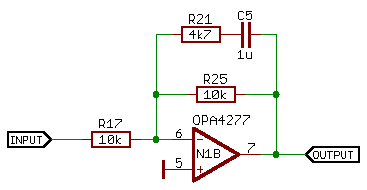
\includegraphics[width=\columnwidth]{graphics/60-hv-amp-dewhitening.pdf}
  \caption[Active inverting dewhitening circuit]{Active inverting dewhitening circuit. This filter uses an inverting op-amp with parallel feedback resistors to achieve the desired frequency response. At low frequencies, the capacitor's impedance is high and so the feedback path is dominated by the impedance of the \SI{10}{\kilo\ohm} resistor and the gain is \num{1}. At high frequencies the capacitor produces very impedance and the feedback path's impedance is the equivalent resistance of the parallel \SI{4.7}{\kilo\ohm} and \SI{10}{\kilo\ohm} resistors and the gain is then $\frac{\SI{10}{\kilo\ohm}}{\SI{3.2}{\kilo\ohm}} \approx \SI{-10}{\deci\bel}$.}
  \label{fig:hv-amp-dewhitening-circuit}
\end{figure}

\begin{figure}
  \centering
  \includegraphics[width=\columnwidth]{graphics/generated/from-python/60-hv-amp-dewhitening-sims.pdf}
  \caption[Simulated dewhitening filter frequency response]{Frequency response of the dewhitening filters simulated with \gls{LISO}. Each dewhitening filter provides \SI{-10}{\deci\bel} gain at high frequencies and so the combined pair produces an overall high frequency gain of $\SI{-20}{\deci\bel} \approx \num{e-1}$.}
  \label{fig:hv-amp-dewhitening-sims}
\end{figure}

\subsubsection{Digital switching electronics}
A series of digital outputs from \gls{CDS} can be used to control the \gls{HV} amplifier's dewhitening filters. The Contec DO-32L-PE output card provides a 32 channel binary switch with an equivalent schematic shown in the left side of Figure\,\ref{fig:hv-amp-sigital-switching}. The control signal from \gls{CDS} for a particular output is inverted and attaches to the negative input of an optocoupler, which acts as a relay without an electrical connection between the input and output. The positive input is attached to a voltage supply such that a digital output of \num{1} results in a closed circuit once inverted. An output of \num{0} is inverted to \num{1} and so there is no potential difference to close the optocoupler's circuit. The optocoupler's output in turn connects to the base of a transistor which controls current flow between the collector and emitter.

\begin{figure}
  \centering
  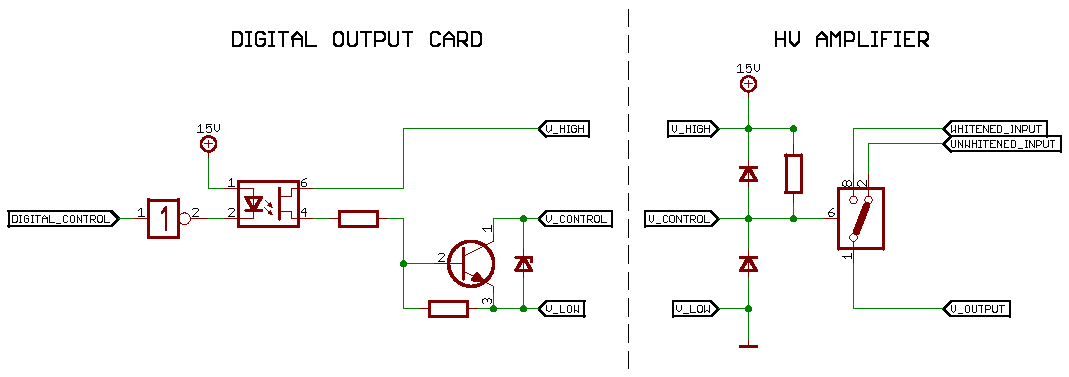
\includegraphics[width=\columnwidth]{graphics/60-hv-amp-digital-switching.pdf}
  \caption[Digital signalling between the control and data acquisition system and a channel within the high voltage amplifier]{\label{fig:hv-amp-sigital-switching}Digital signalling between \gls{CDS} and a channel within the \gls{HV} amplifier. The digital control signal operates an optocoupler which allows current to flow from the $V_{\text{HIGH}}$ voltage reference to a transistor which operates the analogue control signal $V_{\text{CONTROL}}$. This signal is used by the \gls{CMOS} switch in the \gls{HV} amplifier to select either the dewhitened or non-dewhitened signals.}
\end{figure}

The analogue input to the \gls{HV} amplifier for a particular channel is split into two with one passed through the dewhitening filter and the other unperturbed. These two signals form the poles of a \emph{complementary metal-oxide semiconductor} (\gls{CMOS}) switch, chosen for its switching speed, controlled by the digital signal which connects to one of the digital outputs of the \gls{CDS} card via a shielded transmission line. Due to the operation of the digital output card the dewhitening filter control signal $V_{\text{CONTROL}}$ must nominally be $V_{\text{HIGH}}$ which is achieved through the use of a pull-up resistor. When dewhitening is desired, an output of \num{1} at the optocoupler results in a low-resistance path between the control signal and ground and so the control signal within the amplifier becomes $V_{\text{LOW}}$. A truth table is shown in Table\,\ref{tab:digital-dewhitening-truth-table}.

\begin{table}
  \centering
  {\renewcommand{\arraystretch}{1.2} % for extra vertical spacing between rows
    \begin{tabular}{c|c|c}
      \textbf{\gls{CDS} software logic level} & \textbf{$V_{\text{CONTROL}}$} & \textbf{Dewhitening status} \\
      \hline
      0 & $V_{\text{HIGH}}$ & On \\
      1 & $V_{\text{LOW}}$ & Off
    \end{tabular}
  }
  \caption[Truth table for digital switching of dewhitening filters in the high voltage amplifier]{\label{tab:digital-dewhitening-truth-table}Truth table for digital switching of dewhitening filters in the \gls{HV} amplifier, showing the effect that a software logic level in \gls{CDS} has on the dewhitening of the input signal for a particular channel in the \gls{HV} amplifier.}
\end{table}

The electronics shown in Figure\,\ref{fig:hv-amp-sigital-switching} are for a single dewhitener. This configuration must be repeated twice for each of the amplifier's channels to control each of the dewhitening filters.

\subsection{Choice of high voltage op-amp}
Due to the nature of the load the amplifier does not need to drive a significant current, but the voltage noise it produces must be significantly lower than the displacement requirement for the experiment in order for it not to limit its sensitivity. The lowest noise high voltage amplifier integrated circuits available tend to be \gls{MOSFET}-type op-amps. The choice of device tends to be motivated by the bandwidth, maximum output voltage and noise of each particular model.

The \emph{gain-bandwidth product} specifies an op-amp's open-loop gain as a function of the bandwidth it is able to provide it over, and this figure is derived from the speed at which the op-amp's output is able to react to a change in its input (its \emph{slew rate}). The full output voltage is not provided at the unity gain frequency and so a more useful figure of merit is the bandwidth over which the maximum output can be provided. For the \SSMEXPT{} it is expected that radiation pressure and thermal noise will require fast corrections in the \SI{}{\kilo\hertz} range, and to avoid becoming limited by the device's slew rate at higher frequencies (which appears as phase lag on a plot of the frequency response) it is reasonable to require a bandwidth of at least \SI{20}{\kilo\hertz}.

The required \gls{DC} op-amp gain should be known ahead of time in order to fully estimate the effect an op-amp's noise will have on the experiment. The maximum \gls{CDS} input voltage is \SI{\pm10}{\volt} and so to achieve the maximum output voltage requirement when the \gls{CDS} voltage is maximum, thus giving the greatest dynamic range, the op-amp's gain should be set to around \num{40}. From this we can estimate the output noise of some op-amps and determine the Johnson-Nyquist noise (see Section\,\ref{sec:johnson-nyquist-noise}) contribution of the resistors that define the op-amp's \gls{DC} gain.

Table\,\ref{tab:hv-op-amp-comparison} shows the aforementioned parameters for some popular op-amp models. The models shown have sufficient output voltage and identical input noise. The PA89's bandwidth is limited and the full output voltage is not available beyond \SI{7}{\kilo\hertz}, whilst the quiescent power in the PA94 and PA98 is high enough to warrant challenging heat sink requirements. In this case the optimal choice of op-amp is the PA95, for which only a passive heat sink will be required.

\begin{table}
  \centering
  \begin{tabular}{r|c|c|c|c}
    & \textbf{PA89} & \textbf{PA94} & \textbf{PA95} & \textbf{PA98} \\
    \hline
    \textbf{Maximum output} & \SI{1140}{\volt} & \multicolumn{2}{c}{\SI{900}{\volt}} & \SI{450}{\volt} \\
    \textbf{Bandwidth @ \SI{400}{\volt} output} & \SI{7}{\kilo\hertz} & \SI{90}{\kilo\hertz} & \SI{30}{\kilo\hertz} & \SI{60}{\kilo\hertz} \\
    \textbf{Input noise @ \SI{100}{\hertz}} & \multicolumn{4}{c}{\SI{6}{\nano\volt\per\sqrthz}} \\
    \textbf{Quiescent power @ \SI{\pm400}{\volt}} & \SI{3.8}{\watt} & \SI{14.1}{\watt} & \SI{1.3}{\watt} & \SI{17.5}{\watt}
  \end{tabular}
  \caption[Performance specifications for various high voltage operational amplifiers]{\label{tab:hv-op-amp-comparison}Performance specifications for various \gls{HV} op-amps. All of the models listed are manufactured by Apex and the values have been obtained from their respective data sheets. The PA95 was selected due to its low quiescent power for the desired voltage range, which in turn eases the requirement for heat sinking, and the bandwidth is sufficient for the \SSMEXPT{}.}
\end{table}

\subsection{Amplifier signal path}
The amplifier signal path is shown for a single channel in Figure\,\ref{fig:hv-amp-signal-path}. The differential inputs IN+ and IN- are converted to a single-ended signal which is then passed through the two dewhitening stages controlled by digital switches. The signal is then split into two parts, with one part being inverted, before they are input to the PA95 power op-amps. The inputs are clamped together by diodes to ensure that the difference is less than \SI{0.7}{\volt}. This is to prevent the expensive op-amps from damage caused by overvoltage at the inputs, and does not limit the bandwidth or dynamic range in this application. A \SI{1}{\percent} voltage divider at each of the differential outputs provides a signal that is within the input range of \gls{CDS} for the purpose of output monitoring. This provides a readback channel for the controller in order to assist with the calibration of the device.

\begin{figure}
  \centering
  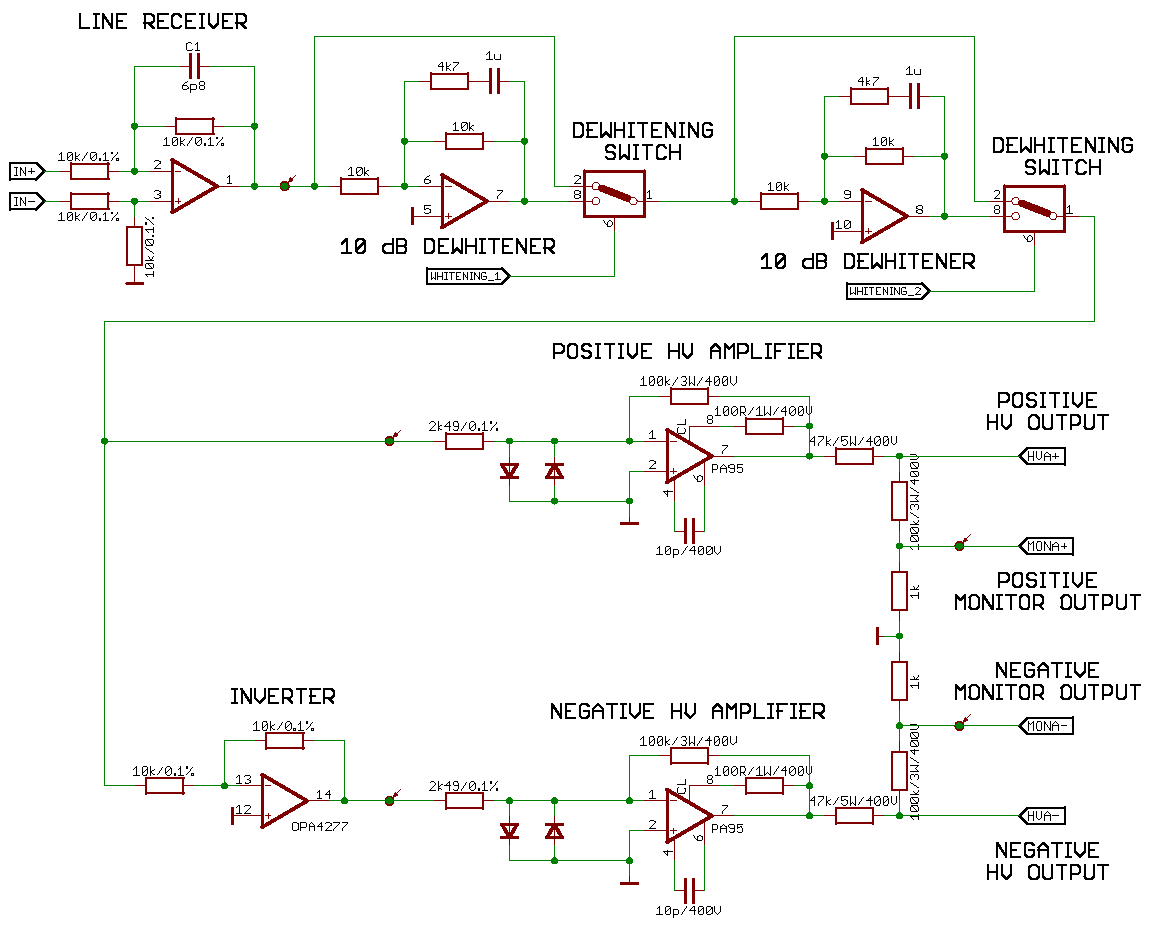
\includegraphics[width=\columnwidth]{graphics/60-hv-amp-signal-path.pdf}
  \caption[High voltage amplifier signal schematic]{\label{fig:hv-amp-signal-path}Schematic of a single high voltage amplifier channel. The input from \gls{CDS} is differentially received, dewhitened and then split into differential outputs that are amplified by PA95 op-amps. A pickoff reads \SI{1}{\percent} of the output voltage for the purposes of calibration.}
\end{figure}

\subsection{Practical and safety features}
As the \gls{HV} amplifier handles potentially lethal current and voltage, a number of additional features beyond the signal circuitry are present.

\subsubsection{Current limiting}
At the output of each \gls{HV} rail there are \SI{47}{\kilo\ohm} resistors which passively limit the current on each rail to around \SI{10}{\milli\ampere}. This operates in addition to an active current limit set via a \SI{100}{\ohm} witness resistor between two pins of each PA95 op-amp. The current limit does not impact the driving of capacitive loads, but ensures that the current produced by the \gls{HV} amplifier is not lethal.

\subsubsection{Soft-start}
Capacitors are present upon the \gls{HV} supply lines to filter \gls{AC} noise, and these must be charged when the device is switched on. Normally these capacitors would present very little impedance to the power supplies and so a large initial current would be drawn, potentially damaging components in its path. The simplest technique to prevent this from happening would be to put resistors in the path of the power supplies, but resistors that would charge the capacitors at a safe rate in a short time would also dissipate a lot of power and require heat sinking. Instead, we use a \emph{soft-start} mechanism which controls the current flow during the charging of the capacitors. The \gls{HV} amplifier's on-off switch operates some optocouplers which allow current to flow into the circuit. Initially, when the circuit's \gls{HV} capacitors are discharged the current on each \gls{HV} rail is limited by the parallel \SI{5}{\kilo\ohm} resistors. A \SI{2.5}{\percent} pick-off from each \gls{HV} rail is compared to a reference \SI{5}{\volt} voltage at an op-amp, the output of which operates a second optocoupler on each rail. When the voltage surpasses \SI{200}{\volt} the power the \SI{5}{\kilo\ohm} resistors dissipate is \SI{8}{\watt}, which is near the reasonable limit for passively cooled resistors. At this point, the capacitors are almost fully charged and the pick-off voltage surpasses the \SI{5}{\volt} reference, and so the op-amp's output operates the optocoupler to open up a low-resistance path that bypasses the \SI{5}{\kilo\ohm} resistors and prevents them from overheating. This is shown in Figure\,\ref{fig:hv-amp-soft-start}.

\begin{figure}
  \centering
  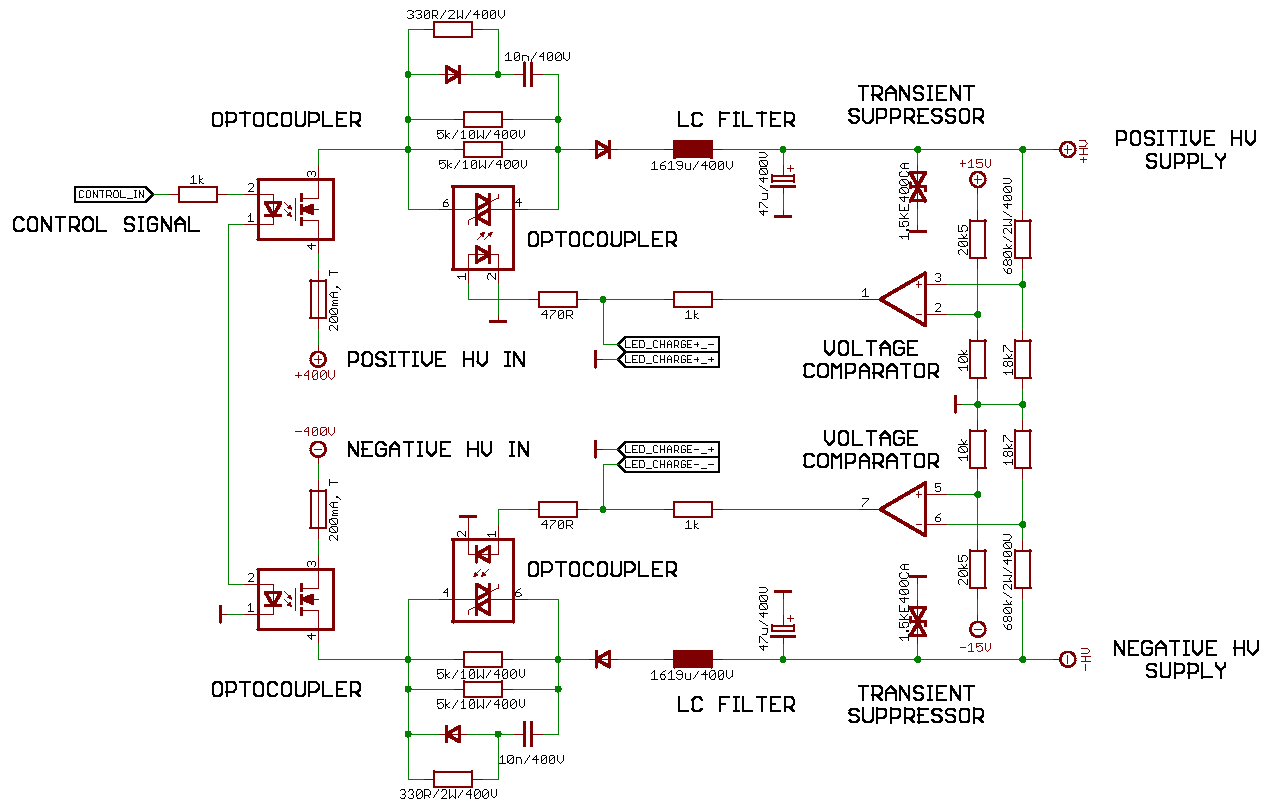
\includegraphics[width=\columnwidth]{graphics/60-hv-amp-soft-start.pdf}
  \caption[High voltage amplifier soft-start schematic]{\label{fig:hv-amp-soft-start}Soft-start mechanism to prevent excessive power supply current draw. This design is based on one the soft-start mechanism for a device produced for the \AEIPROTOTYPE{} by Andreas Weidner. The leftmost optocouplers control whether current is allowed to flow from the power supplies given a control signal from an on-off switch on the enclosure. After the electronics are switched on, the current flow is initially limited by two \SI{5}{\kilo\ohm} resistors. Any \gls{AC} signal content is filtered by the presence of a \SI{1.6}{\milli\farad} choke. A \SI{2.5}{\percent} pick-off from each \gls{HV} rail is compared to a \SI{\pm5}{\volt} reference, with the resulting difference fed back to a second pair of optocouplers which gradually open up a low-resistance path on each supply rail. Without these optocouplers, the power the \SI{5}{\kilo\ohm} resistors would need to dissipate would be considerable at maximum voltage. As the supply voltage increases beyond around \SI{200}{\volt}, the resistance through the optocoupler is reduced far below the \SI{5}{\kilo\ohm} resistors and so the power dissipated in the resistors is negligible.}
\end{figure}

\subsubsection{Pressure and temperature interlock}
The breakdown voltage of the plate capacitors as a function of pressure, given by Paschen's Law, has a minimum in the region of \SI{e-1}{\milli\bar} to \SI{e1}{\milli\bar} depending on the separation and geometry of the anode and cathode, as shown in Figure\,\ref{fig:esd-paschen}. In addition, related effects such as surface tracking can lead to arcing at voltages above \SI{50}{\volt} in low vacuum.

Although the use of high voltage plate capacitors is in general safe at both atmospheric pressure and high vacuum, the act of pumping gas out of the vacuum system necessarily passes through pressures at which arcing can occur. To prevent the possibility of arcing, a cut-off function is present within the circuit to prevent high voltage output unless a control signal is supplied (see Figure\,\ref{fig:hv-amp-interlock}). This signal will be produced by \gls{CDS} derived from a separate pressure monitor. Additionally, as a temperature fail-safe for the amplifier components, temperature sensors are present within the enclosure which operate threshold switches able to remove the supply current via the same mechanism as the pressure interlock. The outputs from each interlock are sent to an AND gate. Only if both the pressure and temperature switches are switched on will the control signal used to operate the \gls{HV} supplies switch on. The interlock circuit is shown in Figure\,\ref{fig:hv-amp-interlock}.
% pressure vs voltage claim from speedmeter labbook, at https://arran.physics.gla.ac.uk/wp/speedmeter/2015/01/30/esd-hv-amplifier-pressure-cutoff/

\begin{figure}
  \centering
  \includegraphics[width=\columnwidth]{graphics/generated/from-python/60-esd-paschen.pdf}
  \caption[Minimum breakdown voltage between the two plates of the electrostatic drive for different separations]{\label{fig:esd-paschen}The minimum breakdown voltage between the two plates of the \gls{ESD} for different separations. This is calculated using Paschen's Law, assuming nitrogen gas and a flat plate geometry. The real effect is a lot more complicated than this model, but the steep slope at lower pressures shown here indicates that the voltage created by the \gls{HV} amplifier for the \gls{ESD} experiment will avoid problems associated with arcing as long as it is operated at atmosphere or high vacuum.}
\end{figure}

\begin{figure}
  \centering
  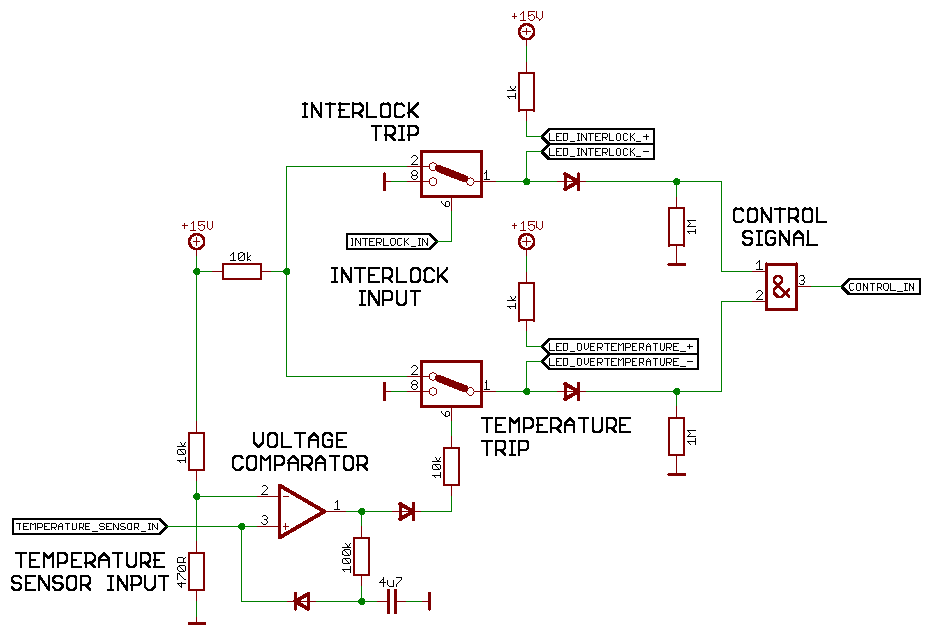
\includegraphics[width=\columnwidth]{graphics/60-hv-amp-interlock.pdf}
  \caption[High voltage amplifier interlock schematic]{\label{fig:hv-amp-interlock}Pressure and temperature interlock circuit. The digital interlock signal from \gls{CDS} operates one switch and the output from a temperature sensor threshold switch operates another. Only if both switches output \SI{15}{\volt} will the control signal used to operate the \gls{HV} supplies switch on.}
\end{figure}

\subsection{Transfer functions and noise measurements}
Transfer functions for the \gls{HV} amplifier can be measured by injecting a known signal into one channel and measuring the corresponding output. The monitor output provides a means of measuring \SI{1}{\percent} of the full \gls{HV} output with a signal that is within the input range of \gls{CDS}.

\subsubsection{Swept sine response of each channel}
Figure\,\ref{fig:hv-amp-dewhitened-tfs} shows the \emph{swept sine} response, calculated by injecting a sine wave at a given frequency, measuring the output signal and dividing it by the injection. These measurements were made without the digital dewhitening switches engaged such that they provide \SI{20}{\deci\bel} of low-pass filtering. The figure shows the response expected from the predictions made by \gls{LISO} shown in Figure\,\ref{fig:hv-amp-dewhitening-sims}.

\begin{figure}
  \centering
  \includegraphics[width=\columnwidth]{graphics/generated/from-python/60-hv-amp-dewhitened-tfs.pdf}
  \caption[Frequency response of the high voltage amplifier's channels with dewhitening enabled]{Second amplifier transfer functions with dewhitening enabled. The expected performance of the dewhitening filter from theory is shown in \checkme{purple} alongside the transfer functions of each channel. The curves agree closely, showing that the implemented filter operates as expected. The mismatch at high frequency is caused by the anti-aliasing filters implemented in \gls{CDS}, which aggressively filter signals above a few \SI{}{\kilo\hertz}.}
  \label{fig:hv-amp-dewhitened-tfs}
\end{figure}

\subsubsection{Response with and without dewhitening}
Figure\,\ref{fig:hv-amp-channel-one-tfs} shows swept sine measurements of the first channel with the dewhitening filters in various states: both on, the first on and the second off, the first off and the second on, and both off. The measurements match predictions and the response with both dewhiteners off is flat as intended across the measurement band.

\begin{figure}
  \centering
  \includegraphics[width=\columnwidth]{graphics/generated/from-python/60-hv-amp-channel-one-tfs.pdf}
  \caption[Transfer functions of the high voltage amplifier input to monitor output with the dewhiteners on and off]{Transfer functions of the high voltage amplifier input to monitor output with the dewhitening filters on and off. The monitor output is a \SI{1}{\percent} pick-off from the main \gls{HV} output, and so the gain is \num{0.4} instead of \num{40}. The curves simulated with \gls{LISO} agree exactly with the measurements within the bandwidth of \gls{CDS}, and beyond around \SI{3}{\kilo\hertz} the transfer functions are suppressed by the anti-aliasing filters on \gls{CDS}'s \glspl{ADC}.}
  \label{fig:hv-amp-channel-one-tfs}
\end{figure}

\subsubsection{Coherence between channels}
The channels should be isolated from one another such that a signal injected at one input does not appear at the output of another. Power supply filtering is implemented using capacitors, inductors and diodes such that there should be minimal cross-coupling between the channels. Figure\,\ref{fig:hv-amp-coherence} shows the coherence for each channel to each other channel, measuring whether the output signal has the same phase angle as the input signal. Coherence of \num{1} indicates that there is causal coupling between the two channels, whereas coherence less than around \num{0.5} is expected from statistical random noise processes. This confirms that a high level of isolation between channels is achieved.

\begin{figure}
  \centering
  \includegraphics[width=\columnwidth]{graphics/generated/from-python/60-hv-amp-coherence.pdf}
  \caption[High voltage amplifier cross-channel coherence]{\gls{HV} amplifier cross-channel normalised coherence. A swept sine was injected into each channel in turn whilst measurements of the output phase were made on all four channels. In each case, only the channel with the injection has coherence of \num{1}, while other channels only show the effect from noise.}
  \label{fig:hv-amp-coherence}
\end{figure}

\subsubsection{Output noise}
\note{Show noise projected into effective test mass displacement, and show how this is smaller than the requirement}

% No data yet
% \section{Experimental test of the electrostatic drive}
% To set requirements on the positioning of the plates, and to build and test the infrastructure for the operation of the \glspl{ESD}, this chapter introduces the design for an experiment to test the new \gls{ESD} design.
% 
% \begin{table}
%   \centering
%   \begin{tabular}{ll}
%     \textbf{Parameter}   & \textbf{Value} \\
%     Mirror diameter      & \SI{30}{\milli\meter} \\
%     Mirror thickness     & \SI{6}{\milli\meter} \\
%     Single plate width   & \SI{30}{\milli\meter} \\
%     Single plate length  & \SI{50}{\milli\meter} \\
%     Nominal plate separation & \SI{40}{\milli\meter} \\
%   \end{tabular}
%   \caption[Plate capacitor and optic parameters for the experiment to test the electrostatic drives for the \SSM{}]{\label{tab:esd-expt-parameters}Plate capacitor and optic parameters for the experiment to test the electrostatic drives for the \SSM{}.}
% \end{table}
% 
% Although the \gls{ESD}, and indeed the \SSM{} experiment, primarily require corrections at lower frequencies where seismic noise is dominant, it is beneficial to utilise an amplifier which can provide actuation up to many tens, if not hundreds, of \SI{}{\kilo\hertz}. This facilitates a transfer function which is flat across the vast majority of each experiment's measurement band, avoiding the roll-off at high frequencies due to the integrated circuits utilised within the high voltage amplifier. A flat transfer function makes the calibration of the actuator plant as part of the overall experiment as simple as possible. Another benefit of having a high bandwidth amplifier is the possibility to use it for common mode control loops, where laser frequency stabilisation can be split between feedback to the laser's piezoelectric transducer and actuators on the test masses.
% 
% The key component of a high bandwidth amplifier is the power op-amp. This class of op-amps typically utilises a \gls{MOSFET} design, and can provide high voltage output given a low voltage input. As an example, the Apex PA95 op-amps used in Advanced LIGO's \glspl{ESD} provide up to \SI{900}{\volt} output up to a frequency of around \SI{15}{\kilo\hertz}, and up to \SI{50}{\volt} at \SI{250}{\kilo\hertz}. The PA98 op-amp, also from Apex, provides an output of \SI{450}{\volt} nominally up to \SI{60}{\kilo\hertz}, potentially up to \SI{500}{\kilo\hertz} for a low capacitive load. For the purposes of this experiment, the choice was made to use the PA98 op-amp to provide the ability to study the effect of the actuator across a very wide bandwidth. To this end, an amplifier circuit utilising the PA98 was built based on a design used for the \AEIPROTOTYPE{}. This design provides up to \SI{\pm350}{\volt} output, and originates from a single-ended, \SI{350}{\volt} amplifier design where the PA98 is especially suited. Two notable modifications have been made, with a view to safety.
% 
% % claim about voltage output of PA95 comes from figure ``Power Response'' on p3 of PA95 datasheet (https://www.apexanalog.com/resources/products/pa95u.pdf)
% % claim about voltage output of PA98 comes from figure 8: ``power Response'' on p7 of PA98 datasheet (https://www.apexanalog.com/resources/products/pa98u.pdf)

\section{Outlook}
Parallel plate capacitor \glspl{ESD} provide a low noise alternative to voice coil actuators for the control of suspended test masses, and it is intended for \glspl{ESD} to be used as the high frequency actuators in the \SSMEXPT{}. In order to provide actuation at the required level, an \gls{HV} signal must be supplied to each \gls{ESD}. The technical design of a \gls{HV} amplifier was presented with the intention to provide actuation at the required level and with low enough noise to meet the requirements of the experiment, and measurements show that the design meets the requirements.
\chapter{\label{c:et-lf-control}Conceptual sensing scheme for the low frequency Einstein Telescope detector}

% sinks
\newcommand{\AS}{AS}
\newcommand{\POP}{POP}
\newcommand{\REFL}{REFL}

% readout ports, I and Q
\newcommand{\ASDC}{$\text{\AS}_{\text{DC}}$}
\newcommand{\ASFIRSTI}{$\text{\AS}_{\num{11}}^{\text{I}}$}
\newcommand{\ASFIRSTQ}{$\text{\AS}_{\num{11}}^{\text{Q}}$}
\newcommand{\ASSECONDI}{$\text{\AS}_{\num{57}}^{\text{I}}$}
\newcommand{\ASSECONDQ}{$\text{\AS}_{\num{57}}^{\text{Q}}$}
\newcommand{\ASSUMI}{$\text{\AS}_{\num{68}}^{\text{I}}$}
\newcommand{\ASSUMQ}{$\text{\AS}_{\num{68}}^{\text{Q}}$}
\newcommand{\ASDIFFI}{$\text{\AS}_{\num{45}}^{\text{I}}$}
\newcommand{\ASDIFFQ}{$\text{\AS}_{\num{45}}^{\text{Q}}$}
\newcommand{\POPDC}{$\text{\POP}_{\text{DC}}$}
\newcommand{\POPFIRSTI}{$\text{\POP}_{\num{11}}^{\text{I}}$}
\newcommand{\POPFIRSTQ}{$\text{\POP}_{\num{11}}^{\text{Q}}$}
\newcommand{\POPSECONDI}{$\text{\POP}_{\num{57}}^{\text{I}}$}
\newcommand{\POPSECONDQ}{$\text{\POP}_{\num{57}}^{\text{Q}}$}
\newcommand{\POPSUMI}{$\text{\POP}_{\num{68}}^{\text{I}}$}
\newcommand{\POPSUMQ}{$\text{\POP}_{\num{68}}^{\text{Q}}$}
\newcommand{\POPDIFFI}{$\text{\POP}_{\num{45}}^{\text{I}}$}
\newcommand{\POPDIFFQ}{$\text{\POP}_{\num{45}}^{\text{Q}}$}
\newcommand{\REFLDC}{$\text{\REFL}_{\text{DC}}$}
\newcommand{\REFLFIRSTI}{$\text{\REFL}_{\num{11}}^{\text{I}}$}
\newcommand{\REFLFIRSTQ}{$\text{\REFL}_{\num{11}}^{\text{Q}}$}
\newcommand{\REFLSECONDI}{$\text{\REFL}_{\num{57}}^{\text{I}}$}
\newcommand{\REFLSECONDQ}{$\text{\REFL}_{\num{57}}^{\text{Q}}$}
\newcommand{\REFLSUMI}{$\text{\REFL}_{\num{68}}^{\text{I}}$}
\newcommand{\REFLSUMQ}{$\text{\REFL}_{\num{68}}^{\text{Q}}$}
\newcommand{\REFLDIFFI}{$\text{\REFL}_{\num{45}}^{\text{I}}$}
\newcommand{\REFLDIFFQ}{$\text{\REFL}_{\num{45}}^{\text{Q}}$}

% readout ports, collapsed
\newcommand{\ASFIRST}{$\text{\AS}_{\num{11}}$}
\newcommand{\ASSECOND}{$\text{\AS}_{\num{57}}$}
\newcommand{\ASSUM}{$\text{\AS}_{\num{68}}$}
\newcommand{\ASDIFF}{$\text{\AS}_{\num{45}}$}
\newcommand{\POPFIRST}{$\text{\POP}_{\num{11}}$}
\newcommand{\POPSECOND}{$\text{\POP}_{\num{57}}$}
\newcommand{\POPSUM}{$\text{\POP}_{\num{68}}$}
\newcommand{\POPDIFF}{$\text{\POP}_{\num{45}}$}
\newcommand{\REFLFIRST}{$\text{\REFL}_{\num{11}}$}
\newcommand{\REFLSECOND}{$\text{\REFL}_{\num{57}}$}
\newcommand{\REFLSUM}{$\text{\REFL}_{\num{68}}$}
\newcommand{\REFLDIFF}{$\text{\REFL}_{\num{45}}$}

\section{The \ET{} facility}
In 2011 a group of scientists primarily based in Europe completed a design study \cite{ET2011} to examine the requirements for a gravitational wave observatory that pushes the \MI{} topology to its limits, while making any newly built facility generic enough to allow for the implementation of new topologies as the state of the art evolves. In this study they laid out the expected improvements in technologies to mitigate fundamental and technical noise sources currently limiting the sensitivity of the third generation of detectors, with a number of practical differences to existing facilities.

The design for the \ET{} targets an increase in sensitivity over \ALIGO{} and \AVIRGO{} by a factor of \num{10} over a wide bandwidth. In order to surpass the sensitivity of the current detectors which already expect to improve upon that of the first generation by an order of magnitude, a number of differences and improvements have been envisaged. The proposed \ET{} facility composes six \DRFPMI{}s split between the three corners of a triangle with \SI{10}{\kilo\meter} edges. The design exploits the geometry to implement interferometers with \SI{10}{\kilo\meter} arms meeting at the three vertices to benefit from the colocation of multiple interferometers.

Seismic noise limits the sensitivity of current generation detectors below \SI{10}{\hertz}, and there are astrophysical advantages to being able to achieve good sensitivity at these frequencies \cite{Sathyaprakash2012}, particularly in the ability to see the inspiral and merger of high mass black hole binary coalescences. The majority of spinning neutron stars discovered via optical techniques have also had orbital frequencies below \SI{10}{\hertz} where fundamental noise limits the ability for the current generation of detectors to see such signals. Signals evolving with frequency, such as the binary black hole merger witnessed as \GWFIRSTEVENT{} \cite{Abbott2016} which was seen for a few tens of \SI{}{\milli\second}, are present at frequencies around \SI{2}{\hertz} for hours. Having this extra observation time provides the possibility not only to better estimate the source parameters but also to track the signal evolution with corresponding changes in the signal recycling cavity tuning to provide optimal sensitivity \cite{Heinzel2002, Simakov2014}. The plan for the \ET{} is to have sufficient sensitivity in this band to provide access to this new science; low frequency sensitivity is difficult to achieve in Earth-based detectors, however.

As discussed in Chapter\,\ref{c:speedmeter-control}, the noise influencing gravitational wave interferometers can be split into groups arising from the sensing of signals and from sources that directly influence the test mass displacement. Sensing noise sources are in general independent of the arm length and test mass parameters and instead rely on the amount of light power and the readout scheme being used. The effect on the strain sensitivity of displacement noise sources, however, typically scales inversely to arm length\footnote{This is not because the displacement noise increases with arm length, but because the response of the interferometer can be improved.}; but because other detector parameters must be re-optimised each new arm length this scaling is non-trivial \cite{Dwyer2015}.

As an example of both the benefits and challenges that longer arms can create, consider the arm cavities within a \FPMI{}. For a given readout technique, longer arms provide better strain sensitivity as shown by Equation\,\ref{eq:freq-to-length}. For a given cavity \emph{g-factor}, which determines the cavity's ability to maintain resonance given small perturbations to the position and alignment of its optics, the size of the reflected beam on the test masses is increased proportionally to the square root of the cavity length increase \cite{Graef2013}. This means that the mirrors must have greater surface area to prevent clipping loss, and the increased spot sizes reduce the coating thermal noise as discussed in Section\,\ref{sec:coating-thermal-noise}. To obtain the maximum coating noise benefit the mirrors must be increased in volume as well as surface area to maintain their aspect ratio \cite{Somiya2009a}, and this in turn means they must be heavier. It is a challenge to obtain sufficient quantities of mirror material of the required purity for detector test masses, but the increased mass leads to a reduction in quantum radiation pressure noise as outlined in Section\,\ref{sec:quantum-rp-noise}.

\subsection{New facility}
As discussed in Section\,\ref{sec:seismic-noise}, seismic noise in current detectors limits the sensitivity at low frequencies and creates challenging control requirements due to the mirror motion created by ground vibrations. The \ET{} interferometers will be \num{100} to \SI{200}{\meter} underground to mitigate seismic noise. This location also helps to limit the impact of gravity gradient noise, as discussed in Section\,\ref{sec:gravity-gradient-noise}, which is expected to become a problem as seismic noise is mitigated.

There are a number of benefits to having multiple detectors located in the same facility. The noise properties across the facility will have a similar impact and so it should be possible to combine the signals from each detector in such a way as to generate a \emph{null stream} that contains noise but not signal \cite{Hewitson2005, Ajith2006}; this will be useful for the characterisation of noise sources and will be particularly beneficial for the new noise sources that may be interrogated due to the increased sensitivity. The arrangement of three detectors in a triangle also allows the facility to be optimally sensitive to gravitational waves from all directions \cite{Winkler1985}, whereas existing single-interferometer detectors are sensitive only to incident signals in the plane of the detector. The use of multiple detectors also allows upgrades to be made to some of the interferometers without losing sky coverage.

\subsection{Xylophone configuration}
To provide maximum astrophysical reach the facility is intended to provide sensitivity across an unprecedented bandwidth, from around \SI{2}{\hertz} to \SI{10}{\kilo\hertz}\textemdash a bandwidth significantly larger than that of existing detectors. It was realised that the most technically feasible option to obtain this bandwidth would be to implement two different types of detector, each optimised to provide good sensitivity in either low or high frequencies \cite{Hild2010}, an idea first proposed for \ALIGO{} \cite{Conforto2004}. In the proposed \emph{ET-D} configuration \cite{Hild2011}, a low power, cryogenic interferometer optimises sensitivity to reduce radiation pressure noise at the expense of shot noise, whilst a high power interferometer optimises high frequency sensitivity through the reduction of shot noise. The projected sensitivity of this arrangement is shown in \checkme{black} in Figure\,\ref{fig:et-d-sensitivity}.

% data from http://www.et-gw.eu/etsensitivities
\begin{figure}
  \centering
  \includegraphics[width=\columnwidth]{graphics/generated/from-python/70-et-d-sensitivity-curves.pdf}
  \caption[Sensitivity curves for the Einstein Telescope]{\label{fig:et-d-sensitivity}Sensitivity of the \ET{} detectors, based on the ET-D design \cite{Hild2011}. \ETLF{} is optimised for low frequencies, \ETHF{} is optimised for high frequencies, and the combination yields sensitivity between \SI{2}{\hertz} and \SI{10}{\kilo\hertz}.}
\end{figure}

\subsubsection{ET-LF}
The low frequency detector consists of a \DRFPMI{} configuration as introduced in Section\,\ref{sec:signal-recycling}, but with a detuned signal recycling cavity. This detuning allows for enhanced sensitivity at the signal recycling cavity pole where the optomechanical dynamics create an optical spring that provides sensitivity below the \gls{SQL} at the spring frequency. The cavities will have \SI{18}{\kilo\watt} of light power, which is considerably lower than that of \ALIGO{} at design sensitivity (\SI{800}{\kilo\watt}), leading to reduced quantum radiation pressure noise at low frequencies. Cryogenic test masses are to be used to facilitate a reduction in thermal noise, and the wavelength of the carrier will be changed from the standard \SI{1064}{\nano\meter} to \SI{1550}{\nano\meter} to utilise lower noise materials at such temperatures. Two filter cavities to facilitate frequency dependent squeezing for the further suppression of quantum noise are also included.

The suspension systems for the main test masses are based on those of the \emph{superattenuator} in \VIRGO{} \cite{Acernese2010}. The proposed \SI{17}{\meter} long pendulum system pushes the longitudinal resonant frequency down from around \SI{1}{\hertz} in existing detectors to \checkme{\SI{0.1}{\hertz}}, providing better attenuation of seismic noise above \SI{2}{\hertz}.

The sensitivity of \ETLF{} is shown in \checkme{blue} in Figure\,\ref{fig:et-d-sensitivity}. The sensitive frequency band is between around \SI{2}{\hertz} and \SI{200}{\hertz}.

\subsubsection{ET-HF}
\ETHF{} takes the designs of \ALIGO{} and \AVIRGO{} and assumes improvements to the test mass coating loss, substrate absorption and available input laser power based on expectations for future research, and adds new technologies such as LG33 cavity modes \cite{Carbone2013} and frequency dependent squeezing \cite{Kimble2001} to reduce coating thermal and quantum noise. The combination of greater arm cavity power, heavier test masses, squeezing and improved coatings and materials will increase sensitivity at frequencies above a few hundred \SI{}{\hertz} beyond the current generation by a factor of around \num{10}, as shown in the \gls{ET} design study.
% sensitivity w.r.t. ALIGO is shown in Figure 5, p14 of design study

The sensitivity of \ETHF{} is shown in \checkme{orange} in Figure\,\ref{fig:et-d-sensitivity}.

\section{\label{sec:et-lf-control-challenges}Control challenges with the \ET{}}
Both \ETLF{} and \ETHF{} will present new challenges to the control of large-scale \DRFPMI{}s. Although \ETHF{} can to some extent be seen as a larger version of \ALIGO{} and \AVIRGO{}, and it may therefore be possible to adapt much of the advance detectors' strategies for both longitudinal and angular control, some aspects such as the use of LG33 modes on a large scale and the presence of parametric instabilities at such high arm cavity powers \cite{Evans2015} require extensive research to understand the implications they may have on control. \ETLF{} will also use a topology that resembles existing generation detectors, but it pushes the sensitivity at low frequencies further down and this presents additional challenges with sensing and noise. This chapter will discuss the longitudinal control of \ETLF{}, focusing in particular on the challenge of controlling the interferometer in its detuned state.

As introduced in Section\,\ref{sec:signal-recycling}, signal recycling cavities can be used to enhance the sensitivity of a detector over a particular frequency band. \emph{Tuned} signal recycling involves holding the signal recycling cavity resonant by ensuring that the carrier light's transmitted phase difference is zero, giving an enhancement below the signal recycling cavity's pole frequency. \emph{Resonant sideband extraction}, meanwhile, involves configuring the signal recycling cavity's tuning in such a way as to provide the greatest sensitive bandwidth, by choosing to make the signal recycling cavity resonant for one of the signal sidebands instead of the carrier. One further signal recycling technique involves the use of radiation pressure induced dynamics. So-called \emph{optical springs} are created when high laser power encounters optical cavities detuned from resonance, and the resulting optomechanical interactions can result in enhanced sensitivity at the spring frequency \cite{Buonanno2002}. \emph{Detuned} signal recycling cavities invoke optical springs to enhance the sensitivity of the interferometer in a narrow band.

\ETLF{} employs a detuned signal recycling cavity to increase the sensitivity of the interferometer at low frequencies. The ability for a detuned signal recycling to shift the most sensitive frequency has been demonstrated in \GEO{} between \SI{200}{\hertz} and \SI{1}{\kilo\hertz} \cite{Hild2006}, however the plan for \ETLF{} is to detune the signal recycling cavity to around \SI{25}{\hertz} which has not been achieved before in a suspended audio-band detector. With tuned signal recycling, where the signal recycling cavity is resonant for the carrier, the sidebands used for control of the differential arm cavity mode are present within the signal recycling cavity with equal amplitude. In detuned operation, where the cavity is not resonant for the carrier, the sidebands have unequal amplitude and some of the interferometer's noise couplings that otherwise cancel at the output in the tuned case no longer cancel \cite{Hild2007}. The phase modulation of the control sidebands, created by \glspl{EOM} on the input path, also gets partially converted to amplitude modulation by the detuning, and this can lead to issues with the dynamic range of any photodetectors used to sense the readout \cite{Grote2007}. Often it can be difficult to find a port at which to sense the motion of the signal recycling cavity decoupled from other cavities, and this effect can be exacerbated by large detunings such as in \ETLF{} where noise cross-couplings can become more significant \cite{Hild2007}.

In the \gls{ET} design study the discussion for \ETLF{} stopped short of a control scheme. The rest of this chapter will discuss a conceptual approach to the control of \ETLF{} and will highlight the future work that must be undertaken before a technical design for the control of \ETLF{} can be produced.

\section{\label{sec:multi-dof-control}Longitudinal control of a \DRFPMI{}}
A successful control scheme for an interferometer must satisfy a number of requirements. When the interferometer is in its uncontrolled state, the control scheme must be able to bring it to the \emph{operating point} where it has the desired response to incident gravitational wave signals in a process called \emph{lock acquisition}. Once at the operating point, it must be robust against small perturbations by controlling the impact of noise and signal nonstationarities. Finally, the signal that represents the gravitational wave channel must have low noise, and therefore high sensitivity, to meet the design goals of the scheme.

The lock acquisition scheme is inextricably linked to the technical environment in which the interferometer will operate, and so it is inappropriate to discuss this while \gls{ET}'s technical design is subject to ongoing research. We will focus our efforts, therefore, on the second and third challenges above. Both \ETLF{} and \ETHF{} will utilise \gls{DC} readout to sense the differential motion of the arm cavities in order to sense the effect of gravitational waves.

\subsection{The dc readout technique}
The standard readout technique for \GEOHF{} and the advanced detectors is \gls{DC} readout \cite{Hild2007, Ward2008, Fricke2012}, a form of homodyne readout that involves a compromise between the best sensitivity and technical complexity. The operating point is kept close to the \emph{dark fringe} (see Section\,\ref{sec:operating-point}) to optimise shot noise and reduce the coupling of technical noise, but a slight offset is introduced between the differential round trip phase of each arm in order to allow some of the carrier light to enter the readout port where it acts as a homodyne local oscillator to the signal sidebands (see Section\,\ref{sec:homodyne-readout}). In practice, this detuning\textemdash of the order \SI{}{\pico\meter} at the arm cavities in \ALIGO{}\textemdash is sufficiently small to allow the required sensitivities to be reached. The light that does enter the output port is, however, pre-filtered by the arm cavities and the impact of laser noise is suppressed by the differential detuning. As the source of local oscillator is a fraction of the light from the cavities to be controlled with the readout, the stability of the local oscillator is guaranteed, as opposed to having a separate degree of freedom to control as with other homodyne techniques. The sensitivity of this readout is furthermore improved with respect to heterodyne techniques \cite{Fricke2012}, and in squeezed interferometers it avoids the need to inject squeezing at \gls{RF} sideband frequencies in addition to the carrier frequency.

\subsection{\label{sec:dofs-of-drfpmi}Degrees of freedom}
The \emph{degrees of freedom} of an interferometer are the non-degenerate ways in which the interferometer's mirrors may move away from the operating point. Each degree of freedom has a different precision requirement, with the most stringent typically being the degree of freedom corresponding to the gravitational wave channel. With \gls{DC} readout there is no local oscillator phase or alignment to independently control and so in a \DRFPMI{} the main degrees of freedom to consider are the arm cavity differential and common modes, the length between the beam splitter and the \glspl{ITM} and the recycling cavity lengths. These are defined in the following sections and the lengths that compose each degree of freedom are shown in Figure\,\ref{fig:et-lf-cavity-lengths}.

\begin{figure}
  \centering
  \includegraphics[width=\columnwidth]{graphics/generated/from-svg/70-cavity-lengths.pdf}
  \caption[Cavity lengths in \ETLF{}]{\label{fig:et-lf-cavity-lengths}Cavity lengths in \ETLF{}. The differential and common arm cavity modes compose $L_{\text{X}}$ and $L_{\text{Y}}$, while the auxiliary power and signal recycling and Michelson cavity lengths are composed of a subset of the distances between the beam splitter and each \gls{ITM} and the distances between each recycling mirror and the beam splitter.}
\end{figure}

The motion of each degree of freedom must be witnessed by a sensor and fed back to actuators to control the relevant length. This is called \emph{linear negative feedback} and the concept of shaping feedback dynamics is discussed in greater detail in the context of suspended interferometers in Chapter\,\ref{c:speedmeter-control}.

\subsubsection{Differential arm cavity length}
Gravitational waves change the length of the arms in a \MI{} differentially and due to the presence of the arm cavities in a \DRFPMI{} changes to the differential arm cavity length represents the motion the main readout is most sensitive to. This length is held close to the dark fringe but with a small offset for \gls{DC} readout. The differential arm cavity length signal can be fed back to the \glspl{ETM} differentially to hold the length at the desired operating point.

We define the differential arm cavity length, \emph{\gls{DARM}}, in terms of the average differential length of the arms:
\begin{equation}
  \label{eq:darm-length}
  \delta L_{\text{DARM}} = \frac{L_{\text{X}} - L_{\text{Y}}}{2}.
\end{equation}

\subsubsection{Common arm cavity length}
In-phase changes in the length of the arms of a \MI{} do not primarily couple to the gravitational wave channel, but it is crucial to control this degree of freedom in order to keep the arm cavities at their operating point which, in a \DRFPMI{}, is the state in which the power in the arm cavities is held near maximum. Noise common to the light entering both arms, particularly from the laser's amplitude and frequency fluctuations as discussed in Section\,\ref{sec:laser-noise}, can, unless corrected, change the resonant condition in the arms. Due to its speed a convenient actuator to control common arm length changes is the laser's crystal, whereupon the application of strain changes the laser's frequency as shown by Equation\,\ref{eq:freq-to-length}. It is also typical to use feedback to an \gls{EOM} for corrections above around \SI{100}{\kilo\hertz}. It is also possible to correct slower, larger drifts with common feedback to the \glspl{ETM} or input optics.

We can define the common arm cavity length, \emph{\gls{CARM}}, in terms of the average length of the arms:
\begin{equation}
  \delta L_{\text{CARM}} = \frac{L_{\text{X}} + L_{\text{Y}}}{2}.
\end{equation}

Any arm cavity length change can be expressed in terms of a linear combination of \gls{DARM} and \gls{CARM}.

\subsubsection{Power and signal recycling cavity lengths}
The power recycling cavity should be resonant for the input light in order to optimally recycle light reflected from the beam splitter back towards the laser, to allow the arm cavity power with respect to the interferometer's input power to be maximised. The power recycling cavity length, \emph{\gls{PRCL}} can be defined in terms of the average distance between the power recycling mirror (\gls{PRM}) and the two \glspl{ITM}:
\begin{equation}
  \label{eq:prcl-length}
  \delta L_{\text{PRCL}} = l_{\text{P}} + \frac{l_{\text{X}} + l_{\text{Y}}}{2}.
\end{equation}

The signal recycling length, along with the signal recycling mirror (\gls{SRM}) transmissivity, determines the bandwidth of the signal extraction and therefore needs controlled in order to keep the interferometer's sensitivity stationary. This length, \emph{\gls{SRCL}}, is defined similarly to \gls{PRCL} in terms of the position of the signal recycling mirror:
\begin{equation}
  \label{eq:srcl-length}
  \delta L_{\text{SRCL}} = l_{\text{S}} + \frac{l_{\text{X}} + l_{\text{Y}}}{2}.
\end{equation}

Control of \gls{PRCL} and \gls{SRCL} can be achieved via corrective feedback to the position of the power and signal recycling mirrors, respectively.

\subsubsection{\label{sec:mich-length}Michelson length}
The length between the beam splitter and the \glspl{ITM} should be held in the dark fringe condition for the carrier to correctly couple the common and differential arm cavity modes to the input and output port of the beam splitter, respectively. In a \DRFPMI{} it must also be held constant to keep the amount of carrier and sideband power in the signal recycling cavity stable, which avoids the need for complicated time-varying control signals. This length, \emph{\gls{MICH}}, can be expressed as the differential length between the beam splitter and the \glspl{ITM}:
\begin{equation}
  \label{eq:mich-length}
  \delta L_{\text{MICH}} = \frac{l_{\text{X}} - l_{\text{Y}}}{2}.
\end{equation}

The \gls{MICH} length is kept constant by feeding back to the positions of the cavity mirrors. Alternatively this feedback can be applied to the beam splitter, but in this case the recycling mirrors must also be moved to avoid influencing \gls{PRCL} or \gls{SRCL}.

There is an apparent degeneracy between the dark fringes produced by the \gls{MICH} and \gls{DARM} degrees of freedom, and so one might expect that the dark fringe offset required for \gls{DC} readout could be applied to the former. While a \gls{DARM} offset has the disadvantage that it involves the creation of an optical spring due to the high light power in the arms\textemdash mechanically coupling the \gls{CARM} and \gls{DARM} modes \cite{Heidmann2011, Vostrosablin2014}\textemdash it has favourable noise couplings compared to a \gls{MICH} offset \cite{Vajente2011}. The \gls{MICH} degree of freedom is filtered above the pole frequency of the power recycling cavity, which is typically at a high frequency, whereas the \gls{DARM} mode is additionally filtered by the arm cavity poles which are usually much lower in frequency.

Note that the common equivalent of the Michelson mode, $\frac{l_{\text{X}} + l_{\text{Y}}}{2}$, has no impact on the interferometer control to first order and so is not considered.

\subsubsection{Driving coefficients}
Table\,\ref{tab:et-lf-driving-coefficients} lists the coefficients to be applied to the error signals representing the degrees of freedom as defined in the previous subsections. Corrections to \gls{CARM} and \gls{DARM} are defined in terms of the positions of the \glspl{ETM}, with the difference between the two degrees of freedom being whether the correction is in-phase or out-of-phase, respectively. The \gls{PRCL} and \gls{SRCL} degrees of freedom are defined as corrections to the power and signal recycling mirrors, respectively. \gls{MICH} is a little more tricky, and as explained in Section\,\ref{sec:mich-length} it can be achieved with feedback either to all of the arm cavity mirrors or to the beam splitter and recycling mirrors. For the purposes of this study we choose the former to avoid the need to correct the unit drive amplitude applied to the beam splitter due to its angle of incidence.

\begin{table}
  \centering
  \begin{tabular}{r|ccccccc}
    & \textbf{\gls{ITM} X} & \textbf{\gls{ETM} X} & \textbf{\gls{ITM} Y} & \textbf{\gls{ETM} Y} & \textbf{\gls{BS}} & \textbf{\gls{PRM}} & \textbf{\gls{SRM}} \\
    \hline
    \gls{CARM} & \num{0} & \num{0.5} & \num{0} & \num{0.5} & \num{0} & \num{0} & \num{0} \\
    \gls{DARM} & \num{0} & \num{0.5} & \num{0} & \num{-0.5} & \num{0} & \num{0} & \num{0} \\
    \gls{MICH} & \num{-0.5} & \num{0.5} & \num{0.5} & \num{-0.5} & \num{0} & \num{0} & \num{0} \\
    \gls{PRCL} & \num{0} & \num{0} & \num{0} & \num{0} & \num{0} & \num{1} & \num{0} \\
    \gls{SRCL} & \num{0} & \num{0} & \num{0} & \num{0} & \num{0} & \num{0} & \num{1} \\
  \end{tabular}
  \caption[Driving coefficients for each mirror and each degree of freedom of \ETLF{}]{\label{tab:et-lf-driving-coefficients}Driving coefficients for each mirror and each degree of freedom of \ETLF{}. \gls{CARM} and \gls{DARM} involve the driving of the \glspl{ETM} in- and out-of-phase, respectively. \gls{MICH} involves moving the \glspl{ITM} differentially, but to avoid sensing \gls{DARM} effects the \glspl{ETM} must be moved too. The driving coefficients are defined with respect to the direction of the \gls{HR} surface of each optic, and as such the coefficients in \gls{MICH} for the \gls{ETM} and \gls{ITM} in each cavity have opposite sign. \gls{PRCL} and \gls{SRCL} involve moving the power and signal recycling mirrors, respectively.}
\end{table}

\subsection{\label{sec:decoupled-sidebands}Decoupled control signals}
In gravitational wave detectors the error signals representing the \gls{DARM} and \gls{CARM} lengths are derived using \emph{modulation/demodulation} schemes, usually variations of the Pound-Drever-Hall technique discussed in Section\,\ref{sec:pdh}. For \MI{}s a number of techniques have been developed such as \emph{internal} and \emph{external} modulation, but the most prominent technique employed in all recent detectors is \emph{Schnupp} modulation. This uses control sidebands imposed on the carrier by means of phase modulation before the light is coupled into the arms by the beam splitter \cite{Heinzel1999}.

In a heterodyne sensing scheme, for the control sidebands to enter the output port to provide an error signal for the arms their lengths must be macroscopically mismatched (by much greater than the wavelength); this is called a \emph{Schnupp asymmetry}. For a Schnupp asymmetry $\Delta l_{\text{SCH}}$, the two arms in a \MI{} have length $l + \frac{\Delta l_{\text{SCH}}}{2}$ and $l - \frac{\Delta l_{\text{SCH}}}{2}$ where the nominal length is $l$. The Schnupp asymmetry differs from the previous microscipic distances defined in Equations \ref{eq:darm-length} to \ref{eq:mich-length} in that it is typically equivalent to many thousands of wavelengths. Although a \DRFPMI{} will typically employ \gls{DC} readout and therefore does not require heterodyne error signals for the control of \gls{DARM}, this asymmetry is required for the control of \gls{SRCL}. The application of a Schnupp asymmetry within a \DRFPMI{} is shown in Figure\,\ref{fig:schnupp-darm-offsets}.

\begin{figure}
  \centering
  \includegraphics[width=\columnwidth]{graphics/generated/from-svg/70-schnupp-darm-offsets.pdf}
  \caption[Schnupp asymmetry and differential arm cavity offset in a \DRFPMI{}]{\label{fig:schnupp-darm-offsets}The Schnupp asymmetry and differential arm cavity offset in a \DRFPMI{}. The Schnupp asymmetry allows the control sidebands resonant in the \MI{} to leave the beam splitter's output port where they may sense the motion of the signal recycling cavity. This is typically an offset of the order of \SI{}{\centi\meter}. The differential arm cavity (\gls{DARM}) offset is a microscopic detuning of the arm cavities to allow a small amount of light to interfere constructively at the beam splitter in order for it to act as a local oscillator to the signal sidebands at the output port. This detuning is typically of the order of \SI{}{\pico\meter}.}
\end{figure}

In a simple \MI{} control sidebands at a single modulation frequency can be imposed upon the carrier to discriminate the phase of the arm cavities with respect to the input, and the modulation frequency is chosen such that the control sidebands will propagate in the interferometer but not enter the arm cavities so that they can act as a phase reference for the light that does. While the Schnupp modulation technique is applicable to \DRFPMI{}s \cite{Heinzel1998}, it is not trivial to decouple the five degrees of freedom when they are sensed by the carrier and a single modulation frequency. For example, the motion of the signal recycling mirror cannot be decoupled from the motion of the power recycling mirror in a single control sideband frequency; instead the signal will contain a linear combination of the motion of the two. By employing a second modulation frequency a suitable phase reference can be obtained for each of the degrees of freedom by carefully arranging for each modulation frequency to resonate in a subset of the cavities to control. Methods to find and create decoupled error signals in a \DRFPMI{} are discussed in the following subsections.

\subsubsection{\label{sec:drfpmi-gain-hierarchy}Gain hierarchy}
Some degrees of freedom require a wider control bandwidth in order for the interferometer to be held at its operating point. For example, laser frequency and intensity noise is present across the measurement band at the input of the interferometer and must be suppressed by many orders of magnitude to be compatible with the sensitivity requirements of a audio-band gravitational wave interferometer. In order to provide high gain within the detection band the bandwidth of the controller (see Appendix\,\ref{sec:control-bandwidth}) is high. Laser noise mainly couples to \gls{CARM} and not to the other degrees of freedom, but control of \gls{CARM} is necessary to maintain light power within the arm cavities, and hence sensitivity. In \ALIGO{} the control bandwidth for \gls{CARM} is \SI{65}{\kilo\hertz} \cite{Abbott2010}. On the other hand, control of \gls{DARM} and the auxiliary degrees of freedom tends to be driven by the presence of low frequency seismic noise and so typically requires much smaller control bandwidth (see for example the differential arm length control precision requirement for the \SSMEXPT{} in Section\,\ref{sec:ssm-required-control}). Through the appropriate selection of servos for each degree of freedom the cross-couplings present at each sensor from secondary degrees of freedom can be suppressed. This is called \emph{gain hierarchy} and has been demonstrated in \LIGO{} \cite{Fritschel2001}.

\subsubsection{\label{sec:sideband-beats}Combination of control sideband frequencies}
Error signals with greater decoupling, particularly for the inner degrees of freedom, can in some cases be found by demodulating the light at some combination of the two sideband frequencies \cite{Strain2003, Barr2006}. Some of the control signals used in \ALIGO{} involve demodulation at the sum or difference of the two sideband frequencies \cite{Abbott2010} or the use of double-demodulation \cite{Staley2014}.

\subsubsection{\label{sec:control-matrix-operations}Control matrix operations}
As the resonant conditions of the control sidebands can be different from the carrier, the magnitude and phase with which error signals representing each degree of freedom appear at each probe can be different.

The gradient of the error signal as witnessed by a sensor for motion of a given degree of freedom represents the interferometer's response for that degree of freedom, as shown for example in Figure\,\ref{fig:pdh-response} for the \SSM{} experiment. A \emph{sensing matrix} can be assembled with the collection of error signal slopes from each degree of freedom in an interferometer to each probe. With this matrix it is then possible to perform row and column operations to suppress cross-couplings in an operation that resembles Gaussian elimination. As the creation of linear combinations of signals can be performed in real time by the controller, the assembly of a \emph{control matrix} based on simulations and used to feed back combinations of error signals to the interferometer's actuators can serve as an approximation to the eventual implementation. This is the starting point for further analysis of the effects of noise coupling from each degree of freedom to the sensors.

Some signals from different degrees of freedom appear with similar magnitude at a particular port and cannot easily be decoupled with gain hierarchy or row and column operations. Instead, the phase of the readout can be used to discriminate between the two error signals. By demodulating each light field at two phases separated by \num{0} and \SI{90}{\degree} with respect to the control sideband modulation frequencies, so-called \emph{I} and \emph{Q} quadrature error signals can be obtained which can later be mixed to suppress the effect of one error signal with respect to another.

\section{Longitudinal sensing scheme for ET-LF}
The following section presents a concept for the longitudinal control of \ETLF{}. Using the techniques discussed in Section\,\ref{sec:multi-dof-control}, we will devise a control scheme based on the approach taken for the second generation detectors, namely through the use of \gls{DC} readout for \gls{DARM} and heterodyne readout for \gls{CARM}, \gls{PRCL}, \gls{SRCL} and \gls{MICH}.

\subsection{Scope and method}
Given the complexity of the interferometer we choose a numerical approach to the modelling and for this we will employ Optickle (see Appendix\,\ref{sec:optickle-sim}) using its plane wave mode. Angular control of the interferometer is expected to present its own challenges given the higher cavity power, larger beams and g-factors closer to unity compared to current generation detectors, but the longitudinal degrees of freedom must be shown to be controllable before angular degrees of freedom can be considered. Future angular sensing and control simulations will be possible with the model developed over the course of this work.

The sensing scheme assumes that the interferometer has been brought close to its operating point by a lock acquisition routine, and here we primarily consider the control of the interferometer in terms of its sensing matrix. It is well known that noise coupling between longitudinal degrees of freedom of detuned \DRFPMI{}s can be significant \cite{Hild2007}, but a crucial initial step before any control noise simulations can be undertaken is the development of a provisional sensing scheme. For \ETLF{} we loosely follow the approach taken for \ALIGO{} \cite{Abbott2010} and \AVIRGO{} \cite{Vajente2008} given that these represent the most sensitive \DRFPMI{}s built to date. To simplify the steps required to produce the scheme the parameters are defined in order from the least to the most constrained. With these parameters fixed we can then search for ports at which error signals representing each degree of freedom can be extracted, and this allows us to define a \emph{sensing matrix} that highlights cross-couplings between each of the degrees of freedom. This is the starting point for control loop noise studies employing gain hierarchy as discussed in Section\,\ref{sec:drfpmi-gain-hierarchy}, which will be the subject of future work.

\subsubsection{Optimal input coupling}
Placing a power recycling mirror before a \MI{}, as discussed in Section\,\ref{sec:power-recycling}, creates an additional cavity between the input and the \glspl{ITM}. The intention of the power recycling mirror is to minimise the light reflected back towards the laser, and in order to do this the cavity it creates should be \emph{impedance matched} (see, for example, Section\,5.1 of \cite{Freise2010}). The loss within the interferometer in combination with the transmissivity of the power recycling mirror $T_{\text{PRM}}$ determines the impedance matching. In the \gls{ET} design study the loss per surface is assumed to be \SI{35}{\ppm} and the transmissivity of the \glspl{ETM} is \SI{6}{\ppm}; both contribute to the total loss. It also suggests the transmissivity of the power recycling mirror to be \SI{4.6}{\percent}. Figure\,\ref{fig:reflected-power-vs-prm-trans} shows the ratio of the light power leaving the power recycling mirror heading back towards the laser to the input light power. The minimum reflected power corresponds to a power recycling mirror transmissivity of \SI{4.6}{\percent}, validating the choice from the \gls{ET} design study. If the scatter or substrate loss of the optics is changed in the future, for instance due to the development of new coatings or the introduction of additional steering mirrors, this model can be used to recalculate the optimum power recycling mirror transmissivity.

\begin{figure}
  \centering
  \includegraphics[width=\columnwidth]{graphics/generated/from-python/70-reflected-power-vs-prm-transmissivity.pdf}
  \caption[Reflected power from \ETLF{} as a function of power recycling mirror transmissivity]{\label{fig:reflected-power-vs-prm-trans}Reflected power from \ETLF{} as a function of power recycling mirror transmissivity. For optimal coupling of the input laser light to the interferometer, the transmissivity of the power recycling mirror must be set to balance the input light with the total loss from the interferometer. For \ETLF{} with loss as per the \gls{ET} design study, this transmissivity should be \SI{4.6}{\percent}.}
\end{figure}

\subsection{\label{sec:control-sideband-freqs}Control sideband frequencies}
In the following subsections we define the constraints on the control sidebands before calculating appropriate frequencies. For a given interferometer it will be possible to find a set of control sideband frequencies any of which will be acceptable for a particular length, but in order for two sideband frequencies to be resonant in a combination of lengths it may be necessary to compromise the resonant conditions such that neither one is optimal for its particular purpose. The case is further complicated by the presence of a detuned signal recycling cavity in \ETLF{}, where the upper and lower control sidebands created with frequencies $-f$ and $+f$ offset from the carrier have different resonant conditions. These issues will be addressed in the following subsections.

\subsubsection{Control sideband resonance in the recycling cavities}
The \SI{310}{\meter} recycling cavity lengths defined in the \gls{ET} design study have \gls{FSR} $\frac{c_0}{2 L_{\text{PRCL}}} = \frac{c_0}{2 L_{\text{SRCL}}} = \SI{483.5}{\kilo\hertz}$. To start, we can try to make the first sideband frequency resonate in the power recycling cavity. As the arm cavities at the operating point reflect the light back towards the power recycling cavity, the resonant condition is a half-integer multiple of the power recycling cavity \gls{FSR}, i.e.:
\begin{equation}
  \label{eq:prc-fsr}
  f_1 = \left(A + \frac{1}{2} \right) \frac{c_0}{2 L_{\text{PRC}}},
\end{equation}
for positive integer $A$.

We can repeat this step for the signal recycling cavity, instead making the second sideband frequency resonant and the first anti-resonant. In this case the resonant condition is an integer multiple of the cavity's \gls{FSR}, i.e.:
\begin{equation}
  \label{eq:src-fsr}
  \begin{split}
    f_1 &\neq B \frac{c_0}{2 L_{\text{SRC}}} \\
    f_2 &= C \frac{c_0}{2 L_{\text{SRC}}},
  \end{split}
\end{equation}
where $B$ and $C$ are again positive integers.

\subsubsection{Avoiding resonance of the control sidebands in the arm cavities}
Any control sideband frequencies used in \ETLF{} must be outside the arm cavity resonances spaced by integer multiples of the arm cavity free spectral range (\gls{FSR}, see Appendix\,\ref{sec:cavity-fom}) in order to allow them to act as a phase discriminant for \gls{CARM} and \gls{DARM}. The \SI{10}{\kilo\meter} arm cavity \gls{FSR} is \SI{14.99}{\kilo\hertz}. As an integer multiple of the arm cavity \gls{FSR} would allow optimal coupling of the sidebands into the arm cavities, one might assume that an odd half-integer multiple would be optimally anti-resonant; however, in this scenario the lower higher-order control sidebands, necessarily created by the phase modulation upon the \gls{EOM} (see Appendix\,\ref{eq:field-phase-bessel}), would become resonant, and so we choose to offset the sideband frequency slightly from the anti-resonant condition. We therefore stipulate two further requirements in addition to Equations \ref{eq:prc-fsr} and \ref{eq:src-fsr}:
\begin{align}
  \label{eq:arm-fsr}
  f_1 &= \left(D_{1} + \delta_{1} \right) \frac{c_0}{2 L_{\text{Arm}}} \\
  f_2 &= \left(D_{2} + \delta_{2} \right) \frac{c_0}{2 L_{\text{Arm}}},
\end{align}
for positive integers $D_{i}$ and small perturbations $\left| \delta_{i} \right| \ll \frac{1}{2}$.

\subsubsection{Control sideband frequencies}
The control sideband frequencies should ideally be \gls{RF}, at least around \SI{10}{\mega\hertz}, to benefit from the noise advantages discussed in Section\,\ref{sec:pdh}. An upper limit of \SI{100}{\mega\hertz} is reasonable given that quadrant photodetectors requiring large surface area will eventually be required for alignment control. Larger surface areas typically lead to greater stray capacitance, limiting the ability of the device to register signals at higher frequencies \cite{Freise2010}.

We chose the first sideband frequency $f_1$ to be \SI{11363101}{\hertz} which for $A = 23$, $D_{1} = 758$ satisfy the requirements and falls within the suitable range. As the light in the signal recycling cavity must first pass through the power recycling cavity, we must ensure that $f_2$ also resonates in the power recycling cavity. This is achieved by choosing the second sideband to be an integer multiple of the first, which is already resonant in the power recycling cavity. To provide ample difference between the first and second sideband frequencies, we chose $f_2 = 5f_1 = \SI{56815505}{\hertz}$. This is separated far enough in frequency from $f_1$ that we can investigate the use of beats between $f_1$ and $f_2$ for control purposes as discussed in Section\,\ref{sec:sideband-beats}.

We assume a modulation depth of \SI{0.1}{\radian} for $f_1$ and $f_2$ to keep the power in higher modulation orders low while allowing for a reasonable amount of light power in the first order. This parameter has little impact on others and can be tuned later to provide for better separation between the two sideband signals on the sensors.

\subsection{Schnupp asymmetry}
In addition to facilitating the control of the signal recycling cavity, the Schnupp asymmetry governs whether the second control sideband frequency couples to both recycling cavities, or just one. A small offset of a few \SI{}{\centi\meter} between the Michelson lengths $l_X$ and $l_Y$ allows for the signal recycling cavity to be resonant for only one of the sideband frequencies, whereas a larger offset of a few tens of \SI{}{\centi\meter} makes both sideband frequencies resonant there \cite{Vajente2008}. Both methods of control are feasible, with the former being implemented in \ALIGO{} \cite{Abbott2010} and the latter in \KAGRA{} \cite{kagra2013}.

Figure\,\ref{fig:sideband-powers-vs-schnupp-detuned} shows the power of the upper and lower sideband fields with respect to the carrier in the recycling cavities of \ETLF{} given the Schnupp asymmetry and recycling cavity lengths with detuned signal recycling. Since the Schnupp asymmetry is a macroscopic length, it is not easily adjusted during operation and so it is necessary to designate this length in the design phase. Here we choose a Schnupp asymmetry that attempts to maximise the difference in power between the two sideband frequencies in the recycling cavities during detuned operation. This is around \SI{0.08}{\meter}. Also observe that a Schnupp asymmetry of \num{0} results in no sideband power in the signal recycling cavity, and that asymmetries of around \SI{0.5}{\meter} result in a situation where both sideband frequencies are resonant in both recycling cavities. In the latter case it would be possible to obtain decoupled control signals through control matrix operations as discussed in Section\,\ref{sec:control-matrix-operations}.

\begin{figure}
  \centering
  \includegraphics[width=\columnwidth]{graphics/generated/from-python/70-sideband-powers-vs-schnupp-detuned.pdf}
  \caption[Power of the control sidebands in the cavities of \ETLF{} in the detuned configuration]{\label{fig:sideband-powers-vs-schnupp-detuned}Power of the control sidebands in the cavities of \ETLF{} during detuned operation. A macroscopic offset, called the \emph{Schnupp asymmetry}, is intentionally introduced to the Michelson length in order to allow the coupling of the sidebands $\pm f_1$ and $\pm f_2$ into the signal recycling cavity for the purposes of control while maintaining the dark fringe condition for the carrier. Here, we choose to allow $\pm f_2$, but not $\pm f_1$, to couple to the recycling cavities. The power is a reasonable estimate for the relative sensitivity of the sidebands in the recycling cavities, and we choose an asymmetry which gives good separation of the power of the sidebands in each cavity, \SI{0.08}{\meter}.}
\end{figure}

\subsubsection{Optimisation of the signal recycling cavity length}
Note the discrepancy between two of the control sideband frequency constraints in Section\,\ref{sec:control-sideband-freqs}: the power and signal recycling cavities cannot both be simultaneously resonant and anti-resonant to $f_1$ and $f_2$ given that $f_2 = 5 f_1$. To resolve this discrepancy we can scan the length of the signal recycling cavity in order to find a position where $f_2$ is resonant and $f_1$ is not, as shown in Figure\,\ref{fig:sideband-powers-srcl-detuned}. This could otherwise have been achieved by changing $f_2$ by a fraction of the signal recycling cavity's \gls{FSR} given the relation between frequency and length shown in Equation\,\ref{eq:freq-to-length}. We can see that changing the signal recycling cavity length from \SI{310}{\meter} to \SI{311.585}{\meter} results in the desired sideband resonance condition for the $+f_2$ sideband. The power of $f_2$ in the power recycling cavity drops as the lower and upper sidebands get critically coupled into the signal recycling cavity. As the signal recycling cavity detuning in \ETLF{} is large, the signal recycling cavity is not resonant for both the upper and lower $f_2$ sidebands (in the tuned signal recycling cavity configuration the upper and lower sidebands are degenerate).

\begin{figure}
  \centering
  \includegraphics[width=\columnwidth]{graphics/generated/from-python/70-sideband-powers-vs-srcl-detuned.pdf}
  \caption[Power of the control sidebands in the signal recycling cavity as a function of length of \ETLF{} in the detuned configuration]{\label{fig:sideband-powers-srcl-detuned}The power in each sideband in each recycling cavity for detuned signal recycling. The nominal signal recycling cavity length defined by the \gls{ET} design study, \SI{310}{\meter}, is not resonant for the second sideband as intended. As the sideband frequencies are different, we can fix this situation by scanning the signal recycling cavity to find a length that is resonant for $f_2$ but not for $f_1$. For the given choice of Schnupp asymmetry, this occurs at a length of \SI{311.585}{\meter} for the upper sideband. The choice to optimise either the upper or lower sideband is arbitrary since both sidebands contribute signal at the readout.}
\end{figure}

In the power recycling cavity, $f_1$ provides an error signal for the power recycling cavity that is a factor of \num{13} larger than that of $f_2$. At the same time, $f_2$ provides an error signal for the length that is \num{650} times larger than the equivalent for $f_1$ in the signal recycling cavity.

\subsection{Dark fringe offset}
As described in Section\,\ref{sec:homodyne-readout}, \gls{DC} readout at the output port of a \DRFPMI{} requires carrier light to be present to act as a phase reference for the signal sidebands. In an interferometer with matched arms there is no classical light at the output (\emph{dark}) port and so a phase asymmetry must be introduced by differentially detuning the arms by a small amount to create the appropriate \emph{dark fringe offset}. In practice, asymmetries within the arms are already present, for example arising from mismatched arm cavity finesse or asymmetric beam splitter reflectivity. As these effects change the amplitude of the light, they appear in a different quadrature to the signal at the output port and so as long as the loss is small the effect on the sensitivity is minimal.
% The effect of imbalanced finesse, reflectivity etc. in the arms is that the AMPLITUDE of the light recombinging at the BS is different, which leads to amplitude fluctuations at the output port. Meanwhile, the GW effect is a change in phase, so this shows up as a phase fluctuation at the output. The resulting superpositions of the two effects are in different quadratures, i.e. 90 degrees out of phase. Loss like this does affect the optimal homodyne angle.

For our model we do not assume any asymmetries and so we can intentionally introduce a dark fringe offset with an offset in the \gls{DARM} degree of freedom. We define the \gls{DARM} offset as a microscopic detuning of the arm cavity lengths, and it is differential such that one arm has length $L + \frac{\delta L_{\text{DARM}}}{2}$ while the other has length $L - \frac{\delta L_{\text{DARM}}}{2}$, where $L$ is the average length. This is depicted in Figure\,\ref{fig:schnupp-darm-offsets} alongside the Schnupp asymmetry.

Figure\,\ref{fig:total-power-vs-darm-offset-detuned} shows the power at the output port and in the arm cavities as a function of \gls{DARM} offset in the detuned configuration. Standard photodetectors used in \ALIGO{} and \AVIRGO{} can handle up to a few \num{10}s of \SI{}{\milli\watt} and this should ideally be the power incident upon the photodetector at the output port to maximise the signal to dark noise ratio. In \ETLF{}, however, the \gls{DARM} offset required to reach this figure would create a significant mismatch in the power of each arm leading to a strong optical spring effect. For an offset of \SI{12}{\pico\meter}, the power at the output can be set to around \SI{10}{\milli\watt} with a difference of around 3\% in the power in the arms, which should be tolerable in terms of sensitivity and noise coupling.

\begin{figure}
  \centering
  \includegraphics[width=\columnwidth]{graphics/generated/from-python/70-total-power-vs-darm-offset-detuned.pdf}
  \caption[Carrier power at the output port of \ETLF{} in detuned configuration as a function of differential arm cavity offset]{\label{fig:total-power-vs-darm-offset-detuned}Carrier power at the output port of \ETLF{} in detuned configuration as a function of differential arm cavity length (\gls{DARM}) offset. The differential arm detuning required to allow carrier light to enter the dark port for \gls{DC} readout involves an increase or decrease in the microscopic length of each arm cavity, and this changes the circulating power. The compromise must be made between the power available to the photodetector for sensing while maintaining reasonably balanced arm cavities to prevent optical springs from influencing the sensitive band and creating additional noise coupling.}
\end{figure}
% See "Stable optical spring in the Advanced LIGO detector with unbalanced arms and in the Michelson-Sagnac interferometer", equations 6f and 6g show a small part of the common mode entering the differential, and vice versa. Another way of looking at this is to say that the DARM offset at the point of maximum arm cavity power (for one arm) is compensating the detuned signal recycling such that the compound cavity formed by the SRM and (e.g.) the X arm is resonant. This explains the shape of the arm cavity power vs DARM offset.

\subsection{Power in each light field}
The power in each field within each relevant space or cavity of the interferometer is shown in Tables\,\ref{tab:et-lf-detuned-dc-powers} for the detuned interferometer.

\begin{table}
  \centering
  \resizebox{16cm}{!}{%
    \begin{tabular}{r|ccccccccc|c}
      & \textbf{-68 MHz} & \textbf{-57 MHz} & \textbf{-45 MHz} & \textbf{-11 MHz} & \textbf{Carrier} & \textbf{11 MHz} & \textbf{45 MHz} & \textbf{57 MHz} & \textbf{68 MHz} & \textbf{Total} \\
      \hline
      \textbf{Input from laser} & 0 & 0 & 0 & 0 & \SI{3}{\watt} & 0 & 0 & 0 & 0 & \SI{3}{\watt} \\ 
      \textbf{After modulators} & \SI{19}{\micro\watt} & \SI{7}{\milli\watt} & \SI{19}{\micro\watt} & \SI{7}{\milli\watt} & \SI{3}{\watt} & \SI{7}{\milli\watt} & \SI{19}{\micro\watt} & \SI{7}{\milli\watt} & \SI{19}{\micro\watt} & \SI{3}{\watt} \\ 
      \textbf{Power recycling cavity} & \SI{220}{\nano\watt} & \SI{521}{\milli\watt} & \SI{220}{\nano\watt} & \SI{410}{\milli\watt} & \SI{65}{\watt} & \SI{407}{\milli\watt} & \SI{220}{\nano\watt} & \SI{34}{\milli\watt} & \SI{220}{\nano\watt} & \SI{66}{\watt} \\ 
      \textbf{Power recycling pick-off} & \SI{33}{\pico\watt} & \SI{78}{\micro\watt} & \SI{33}{\pico\watt} & \SI{61}{\micro\watt} & \SI{9}{\milli\watt} & \SI{61}{\micro\watt} & \SI{33}{\pico\watt} & \SI{4}{\micro\watt} & \SI{33}{\pico\watt} & \SI{10}{\milli\watt} \\ 
      \textbf{Michelson cavity} & \SI{131}{\nano\watt} & \SI{228}{\milli\watt} & \SI{112}{\nano\watt} & \SI{208}{\milli\watt} & \SI{33}{\watt} & \SI{204}{\milli\watt} & \SI{107}{\nano\watt} & \SI{27}{\milli\watt} & \SI{115}{\nano\watt} & \SI{33}{\watt} \\ 
      \textbf{Arm cavity X} & \SI{261}{\pico\watt} & \SI{557}{\micro\watt} & \SI{375}{\pico\watt} & \SI{9}{\milli\watt} & \SI{18}{\kilo\watt} & \SI{9}{\milli\watt} & \SI{357}{\pico\watt} & \SI{65}{\micro\watt} & \SI{230}{\pico\watt} & \SI{18}{\kilo\watt} \\ 
      \textbf{Arm cavity Y} & \SI{182}{\pico\watt} & \SI{722}{\micro\watt} & \SI{361}{\pico\watt} & \SI{9}{\milli\watt} & \SI{18}{\kilo\watt} & \SI{9}{\milli\watt} & \SI{379}{\pico\watt} & \SI{68}{\micro\watt} & \SI{210}{\pico\watt} & \SI{18}{\kilo\watt} \\ 
      \textbf{Signal recycling cavity} & \SI{3}{\nano\watt} & \SI{4}{\milli\watt} & \SI{379}{\pico\watt} & \SI{69}{\micro\watt} & \SI{15}{\milli\watt} & \SI{41}{\micro\watt} & \SI{411}{\pico\watt} & \SI{26}{\milli\watt} & \SI{928}{\pico\watt} & \SI{45}{\milli\watt} \\ 
      \textbf{Reflected back to laser} & \SI{19}{\micro\watt} & \SI{6}{\milli\watt} & \SI{19}{\micro\watt} & \SI{7}{\milli\watt} & \SI{62}{\micro\watt} & \SI{7}{\milli\watt} & \SI{19}{\micro\watt} & \SI{2}{\milli\watt} & \SI{19}{\micro\watt} & \SI{23}{\milli\watt} \\ 
      \textbf{Output} & \SI{558}{\pico\watt} & \SI{756}{\micro\watt} & \SI{76}{\pico\watt} & \SI{14}{\micro\watt} & \SI{3}{\milli\watt} & \SI{8}{\micro\watt} & \SI{82}{\pico\watt} & \SI{5}{\milli\watt} & \SI{186}{\pico\watt} & \SI{9}{\milli\watt}
    \end{tabular}
  }
  \caption[Light power in \ETLF{} in the detuned configuration]{\label{tab:et-lf-detuned-dc-powers}Powers in various parts of \ETLF{} in the detuned configuration. The input light is passed through \glspl{EOM} which impart control sidebands at two pairs of frequencies offset from the carrier. As the arm cavity \gls{FSR} is \checkme{higher} than that of the control sideband frequencies, the sideband light power in the arms is vastly smaller than the carrier power. The first sideband at $\SI{\pm11}{\mega\hertz}$ is resonant within the power recycling cavity. The second sideband at $\SI{\pm57}{\mega\hertz}$ is resonant within both the power and signal recycling cavities, with the \SI{-57}{\mega\hertz} sideband almost exactly resonant in the power recycling cavity and the +\SI{57}{\mega\hertz} sideband exactly resonant in the signal recycling cavity. The power reflected back towards the laser is composed mainly of light at the two sideband frequencies, as the transmissivity of the power recycling mirror minimises the reflected carrier light. At the output port, the carrier power is present due to the \gls{DARM} offset, and acts as a local oscillator to the signal sidebands there.}
\end{table}

\subsection{\label{sec:etlf-readout-ports}Readout ports}
Figure\,\ref{fig:dof-readouts} shows some available readout ports for \ETLF{} where the sidebands and carrier may be measured for the purposes of control:
\begin{itemize}
  \item \textbf{REFL} (\emph{reflected}) senses the light reflected from the interferometer back towards the input laser;
  \item \textbf{POP} (\emph{pick off \gls{PRCL}}) senses the light in the power recycling cavity;
  \item \textbf{AS} (\emph{asymmetric}) senses the light at the output port of the \DRFPMI{}.
\end{itemize}

\begin{figure}
  \centering
  \includegraphics[width=\columnwidth]{graphics/generated/from-svg/70-dof-readouts.pdf}
  \caption[Some available readout ports for sensing and control in \ETLF{}]{\label{fig:dof-readouts}Some available readout ports for sensing motion of the degrees of freedom in \ETLF{}. Phase modulation sidebands are imparted upon the input laser light at two primary frequencies before it enters the interferometer. Photodetectors are placed at three ports to sense the carrier and these sidebands for the purposes of sensing and control. The most important readout is \AS{}, which strongly senses \gls{DARM}, and this is placed in transmission of the signal recycling mirror. Light reflected back towards the laser is sensed via a Faraday isolator at the \REFL{} port, and a pick-off\textemdash \POP{}\textemdash senses light in the power recycling cavity.}
\end{figure}

For the purposes of the control simulations, each readout port contains incident fields at the carrier frequency and offsets of $\pm f_1$ (\SI{\pm11}{\mega\hertz}), $\pm f_2$ (\SI{\pm57}{\mega\hertz}), $-f_1 - f_2$ (\SI{-68}{\mega\hertz}), $f_1 - f_2$ and $-f_2 + f_1$ (\SI{-45}{\mega\hertz}\footnote{This is not \SI{-46}{\mega\hertz} due to rounding.}), $-f_1 + f_2$ and $f_2 - f_1$ (\SI{45}{\mega\hertz}), and $f_1 + f_2$ (\SI{68}{\mega\hertz}). There are therefore \num{9} light fields propagated through the interferometer that are combined into signals at \num{5} frequencies at \num{3} ports. We furthermore demodulate in the \emph{I} and \emph{Q} quadratures to be able to calculate the optimal readout phase at each port given the propagation delay between each mirror and each sensor. These are shown in Table\,\ref{tab:et-lf-probes}.

\begin{table}
  \centering
  {\renewcommand{\arraystretch}{1.2} % for extra vertical spacing between rows
    \begin{tabular}{r|ccc}
      \textbf{Offset} & \textbf{Output port} & \textbf{Power recycling cavity pick-off} & \textbf{Reflected light pick-off} \\
      \hline
      \num{0} & \ASDC{} & \textemdash & \textemdash \\
      $\pm f_1$    & \ASFIRSTI{}, \ASFIRSTQ{} & \POPFIRSTI{}, \POPFIRSTQ{} & \REFLFIRSTI{}, \REFLFIRSTQ{} \\
      $\pm f_2$    & \ASSECONDI{}, \ASSECONDQ{} & \POPSECONDI{}, \POPSECONDQ{} & \REFLSECONDI{}, \REFLSECONDQ{} \\
      $\pm \left( f_2 - f_1 \right)$ & \ASDIFFI{}, \ASDIFFQ{} & \POPDIFFI{}, \POPDIFFQ{} & \REFLDIFFI{}, \REFLDIFFQ{} \\
      $\pm \left( f_1 + f_2 \right)$ & \ASSUMI{}, \ASSUMQ{} & \POPSUMI{}, \POPSUMQ{} & \REFLSUMI{}, \REFLSUMQ{}
    \end{tabular}
  }
  \caption[Probes that sense the light fields propagating within \ETLF{}]{\label{tab:et-lf-probes}Probes that sense the light fields propagating within \ETLF{} with respect to the carrier frequency. The carrier is sensed by \ASDC{} at the interferometer's output port, which is the light that propagates through the signal recycling mirror. The control sidebands, and the beats between the sidebands, are sensed at the same port demodulated at each relevant frequency, along with similar readouts sensing a small transmission of light through a folding mirror in the power recycling cavity (\POP{}) and the light reflected from the interferometer (\REFL{}).}
\end{table}

\subsection{Control signals}
The sensing matrix, as introduced in Section\,\ref{sec:control-matrix-operations}, can be calculated for \ETLF{} by exciting each degree of freedom with the driving coefficients shown in Table\,\ref{tab:et-lf-driving-coefficients} and measuring the response at each probe shown in Table\,\ref{tab:et-lf-probes}.

At this preliminary stage, a reasonable choice of error signals from the sensing matrix to use for control can be determined through a heuristic approach building upon knowledge gained from the control of the second generation detectors. As $f_2$ resonates in both recycling cavities, it samples the motion of the mirrors that influence \gls{MICH} and \gls{SRCL} as well as \gls{PRCL}. Conversely, $f_1$ only strongly samples the motion of \gls{MICH} and \gls{PRCL}. Using demodulations at these frequencies, and combinations thereof, it should be possible to find a set of reasonably decoupled error signals for each degree of freedom.

\subsubsection{Combination of readout quadratures}
Table\,\ref{tab:et-lf-probes} shows signals at both the $I$ and $Q$ quadratures for all of the \gls{RF} sideband frequencies considered. These quadratures can be combined electronically to produce an error signal with optimal gradient. The exact phase corresponding to the greatest magnitude is not important, as this can be influenced by technical factors such as the length of \gls{RF} transmission lines, but the relative phase between maximum error signals from different degrees of freedom on the same sensor is. If error signals from different degrees of freedom have the same maximum signal at the same or opposite phase, one cannot be minimised with respect to the other through appropriate choice of demodulation phase. On the other hand, if two degrees of freedom couple to a pair of $I$ and $Q$ sensors with equal magnitude but separate phase, they can be used to sense both degrees of freedom. In practice due to temperature drifts and other time-varying effects it is difficult to maintain the demodulation phase of a set of sensors to a precision better than around \SI{1}{\degree} \cite{Effler2014}, and so the readout quadratures chosen for each of the degrees of freedom of \ETLF{} should ideally be separated by many degrees.

\subsubsection{Sensing matrix for ET-LF in detuned configuration}
The sensing matrix for the detuned configuration given the readout ports defined in Table\,\ref{tab:et-lf-probes} is shown in Table\,\ref{tab:et-lf-sensing-matrix-detuned} for mirror perturbations at \gls{DC}. The suggested readouts for each degree of freedom are highlighted in bold and are described in the following text.

The gravitational wave signal will primarily affect \gls{DARM}, and this is by design sensed by \ASDC{}. The common mode loop can be sensed at \REFLFIRST{}. The \gls{MICH}, \gls{PRCL} and \gls{SRCL} cavity error signals are difficult to separate due to the cross-coupling of control sidebands via the Schnupp asymmetry and the sideband asymmetry created by the presence of a detuned signal recycling cavity \cite{Hild2007}. As the control system will be implemented in a \LIGO{} \gls{CDS}-style system \cite{Bork2010}, it will be possible to define in software error signals formed from linear combinations of different sensor signals that decouple other degrees of freedom from a particular readout, as discussed in Section\,\ref{sec:control-matrix-operations}. In Table\,\ref{tab:et-lf-sensing-matrix-detuned}, \gls{PRCL} is dominant over \gls{MICH} and \gls{SRCL} at \POPFIRST{} and so this represents a good extraction point for the motion of the power recycling cavity. \gls{MICH} couples strongly to a number of ports but alongside strong signals from the other degrees of freedom. Its strongest ports, \ASDC{} and \ASSECOND{}, contain much larger signals from \gls{DARM} due to the difference in finesse between the Michelson and the arm cavities, and this would be difficult to remove electronically given the phase degeneracy. A better readout could be to use \POPSECOND{} with the dominant \gls{PRCL} signal suppressed with careful tuning of the demodulation phase. Residual \gls{PRCL} coupling can be subtracted electronically.

\gls{SRCL} is difficult to sense with $\pm f_1$ because they are not resonant in the signal recycling cavity, nor a single demodulation at $\pm f_2$ because these error signals are contaminated with contributions from \gls{MICH} or \gls{PRCL} given the cross-coupling facilitated by the Schnupp asymmetry. A possible sensing strategy could utilise the beats between sidebands found at \REFLDIFF{} or \REFLSUM{} where the contribution from \gls{MICH} and \gls{PRCL} can be suppressed with suitable choice of demodulation phase. All \gls{SRCL} signals contain an offset from zero due to the detuning, since $-f_2$ is not resonant when the signal recycling mirror is at its operating point (see Figure\,\ref{fig:sideband-powers-srcl-detuned}). To use \REFLSUM{} for \gls{SRCL} control an offset equivalent to \SI{-4.2}{\milli\watt} will be necessary.

\begin{table}
  \centering
  \resizebox{16cm}{!}{%
    {\renewcommand{\arraystretch}{1.2} % for extra vertical spacing between rows
      \begin{tabular}{r|ccccc}
	& \textbf{CARM} & \textbf{DARM} & \textbf{MICH} & \textbf{PRCL} & \textbf{SRCL} \\ 
	\hline
	\hline
	\textbf{\ASDC{}} & \num{1.44e+06} (\SI{180.00}{\degree}) & \red{\textbf{\num{4.99e+08}} (\SI{180.00}{\degree})} & \num{1.17e+06} (\SI{180.00}{\degree}) & \num{1.21e+05} (\SI{180.00}{\degree}) & \num{1.39e+04} (\SI{180.00}{\degree}) \\ 
	\textbf{\ASFIRST{}} & \num{2.25e+06} (\SI{-32.56}{\degree}) & \num{3.00e+07} (\SI{55.83}{\degree}) & \num{6.25e+04} (\SI{56.09}{\degree}) & \num{7.54e+03} (\SI{77.99}{\degree}) & \num{1.09e+03} (\SI{58.46}{\degree}) \\ 
	\textbf{\ASSECOND{}} & \num{1.76e+08} (\SI{-112.30}{\degree}) & \num{3.98e+08} (\SI{-162.68}{\degree}) & \num{8.39e+05} (\SI{-163.43}{\degree}) & \num{6.03e+05} (\SI{-78.31}{\degree}) & \num{6.73e+04} (\SI{94.85}{\degree}) \\ 
	\textbf{\ASDIFF{}} & \num{4.71e+04} (\SI{178.86}{\degree}) & \num{3.52e+03} (\SI{107.72}{\degree}) & \num{3.43e+04} (\SI{85.09}{\degree}) & \num{6.44e+04} (\SI{61.41}{\degree}) & \num{3.41e+03} (\SI{-146.01}{\degree}) \\ 
	\textbf{\ASSUM{}} & \num{1.00e+05} (\SI{-177.46}{\degree}) & \num{4.43e+04} (\SI{-83.81}{\degree}) & \num{5.97e+04} (\SI{43.44}{\degree}) & \num{5.13e+04} (\SI{103.97}{\degree}) & \num{4.67e+03} (\SI{-22.78}{\degree}) \\
	\hline
	\textbf{\POPFIRST{}} & \num{7.61e+07} (\SI{-144.47}{\degree}) & \num{6.88e+05} (\SI{-144.49}{\degree}) & \num{8.70e+02} (\SI{-26.41}{\degree}) & \red{\textbf{\num{2.55e+05}} (\SI{-36.40}{\degree})} & \num{3.08e+01} (\SI{-81.49}{\degree}) \\ 
	\textbf{\POPSECOND{}} & \num{5.27e+07} (\SI{99.38}{\degree}) & \num{4.72e+05} (\SI{92.38}{\degree}) & \red{\textbf{\num{2.95e+04}} (\SI{50.72}{\degree})} & \num{1.26e+05} (\SI{-130.50}{\degree}) & \num{1.08e+04} (\SI{120.38}{\degree}) \\ 
	\textbf{\POPDIFF{}} & \num{2.01e+02} (\SI{-51.56}{\degree}) & \num{9.34e+01} (\SI{-127.43}{\degree}) & \num{1.24e+03} (\SI{1.97}{\degree}) & \num{1.61e+04} (\SI{88.80}{\degree}) & \num{1.07e+03} (\SI{167.69}{\degree}) \\ 
	\textbf{\POPSUM{}} & \num{4.94e+02} (\SI{-22.60}{\degree}) & \num{9.93e+01} (\SI{-15.51}{\degree}) & \num{1.07e+03} (\SI{45.23}{\degree}) & \num{8.34e+03} (\SI{-145.33}{\degree}) & \num{1.07e+03} (\SI{-149.81}{\degree}) \\
	\hline
	\textbf{\REFLFIRST{}} & \red{\textbf{\num{1.44e+10}} (\SI{-0.01}{\degree})} & \num{1.31e+08} (\SI{-0.01}{\degree}) & \num{2.34e+05} (\SI{4.53}{\degree}) & \num{5.01e+07} (\SI{-0.41}{\degree}) & \num{2.25e+04} (\SI{45.05}{\degree}) \\ 
	\textbf{\REFLSECOND{}} & \num{4.63e+09} (\SI{-75.19}{\degree}) & \num{5.69e+07} (\SI{-86.52}{\degree}) & \num{1.47e+05} (\SI{-83.24}{\degree}) & \num{1.58e+07} (\SI{-76.05}{\degree}) & \num{1.67e+04} (\SI{30.68}{\degree}) \\ 
	\textbf{\REFLDIFF{}} & \num{3.90e+06} (\SI{0.94}{\degree}) & \num{1.31e+06} (\SI{0.04}{\degree}) & \num{2.19e+05} (\SI{163.21}{\degree}) & \num{1.28e+06} (\SI{-171.17}{\degree}) & \num{2.03e+05} (\SI{-25.15}{\degree}) \\
	\textbf{\REFLSUM{}} & \num{4.04e+06} (\SI{-101.97}{\degree}) & \num{1.32e+06} (\SI{-101.79}{\degree}) & \num{2.25e+05} (\SI{-76.80}{\degree}) & \num{1.40e+06} (\SI{-53.54}{\degree}) & \red{\textbf{\num{2.03e+05}} (\SI{89.52}{\degree})}
      \end{tabular}
    }
  }
  \caption[Gradients of the error signals from each degree of freedom to each probe in \ETLF{} at dc]{\label{tab:et-lf-sensing-matrix-detuned}Gradients of the error signals from each degree of freedom to each probe, in units of \SI{}{\watt\per\meter}, in \ETLF{} at \gls{DC}. The suggested readout probes for each degree of freedom are shown in bold red. The $I$ and $Q$ quadratures of each readout have been combined into a single magnitude and the phase representing the greatest slope and the phase at which it is achieved. The \ASDC{} does not get demodulated but it has phase of \SI{0}{\degree} or \SI{180}{\degree} depending on the sign of the error signal. The \gls{RF} probes contain maximum slopes at phase angles determined by the propagation of the control sidebands through the interferometer. Probes can be optimised to sense the motion of a particular degree of freedom by adjusting the angle at which the sensor $I$ and $Q$ quadratures are combined, but signals on sensors that contain strong signals from other degrees of freedom at nearby phase angles are difficult to use.}
\end{table}

Table\,\ref{tab:et-lf-sensing-matrix-detuned-normalised} shows the gradient of each degree of freedom's error signal at each of the suggested sensors. The values have been normalised with respect to the degree of freedom to be read out. This table shows that the hierarchical control techniques discussed in Section\,\ref{sec:decoupled-sidebands} will be necessary in order to decouple the individual degrees of freedom.

\begin{table}
  \centering
  {\renewcommand{\arraystretch}{1.2} % for extra vertical spacing between rows
    \begin{tabular}{r|ccccc}
      & \textbf{CARM} & \textbf{DARM} & \textbf{MICH} & \textbf{PRCL} & \textbf{SRCL} \\ 
      \hline
      \hline
      \textbf{\REFLFIRST{}} & \red{\textbf{\num{1.0}}} & \num{9.1e-3} & \num{1.6e-5} & \num{3.5e-3} & \num{1.6e-6} \\
      \textbf{\ASDC{}} & \num{2.8e-3} & \red{\textbf{\num{1.0}}} & \num{2.3e-3} & \num{2.4e-4}  & \num{2.8e-5} \\
      \textbf{\POPSECOND{}} & \num{1.8e3} & \num{1.6e1} & \red{\textbf{\num{1.0}}} & \num{4.3e0} & \num{3.7e-1} \\
      \textbf{\POPFIRST{}} & \num{3.0e2} & \num{2.7e0} & \num{3.4e-3} & \red{\textbf{\num{1.0}}} & \num{1.2e-4} \\
      \textbf{\REFLSUM{}} & \num{2.0e1} & \num{6.5e0} & \num{1.1e0} & \num{6.9e0} & \red{\textbf{\num{1.0}}}
    \end{tabular}
  }
  \caption[Normalised gradients of the suggested sensors to be used for the control of \ETLF{}'s degrees of freedom]{\label{tab:et-lf-sensing-matrix-detuned-normalised}Normalised gradients of the suggested sensors to be used for the control of \ETLF{}'s degrees of freedom. Each row from Table\,\ref{tab:et-lf-sensing-matrix-detuned} corresponding to a sensor used to control a degree of freedom has been scaled by the gradient of the error signal corresponding to the respective degree of freedom. This shows the prominence of the other degrees of freedom on each sensor without having applied any of the other control techniques as discussed in Section\,\ref{sec:decoupled-sidebands}.}
\end{table}

Error signals corresponding to the suggested readouts for each degree of freedom are shown in Figure\,\ref{fig:sweeps-et-lf}. These are produced by calculating the power on each sensor at the relevant demodulation frequency as the mirrors are driven as shown in Table\,\ref{tab:et-lf-driving-coefficients} and represent the low-frequency limit of the transfer functions of each degree of freedom to each sensor.

\begin{figure}
  \centering
  \includegraphics[width=\columnwidth]{graphics/generated/from-python/70-sweeps-detuned.pdf}
  \caption[Sweeps through the zero-crossings of the chosen error signals in ET-LF]{\label{fig:sweeps-et-lf}Sweeps through the zero-crossings of the chosen error signals in \ETLF{} in the detuned configuration. Each error signal is linear about the operating point, which ensures a simple, bipolar error signal is available for the purposes of controlling each associated degree of freedom. This linearity has a different range for each readout, with \gls{CARM} and \gls{DARM} requiring the greatest precision.}
\end{figure}

Figure\,B shows the \ASDC{} readout, and the slope is zero when the arm cavities are tuned, consistent with Figure\,\ref{fig:total-power-vs-darm-offset-detuned}, showing that some classical carrier light power is required for \gls{DC} readout. Figure\,E shows the error signal crossing the operating point at a power of \SI{4.2}{\milli\watt}, showing the requirement for an offset.

\subsection{Sensitivity of the scheme}
The sensitivity for \ETLF{} shown in Figure\,\ref{fig:et-d-sensitivity} assumes that the interferometer contains squeezed vacuum input via two filter cavities in addition to the presence of seismic and other noise, and these features have not been modelled in this work. A comparison is shown in Figure\,\ref{fig:et-lf-control-scheme-sensitivity} between the quantum noise limited sensitivity for \ETLF{} in the absence of squeezing, as calculated by the tool used to present the results in the ET-D study \cite{Hild2011}, \gls{GWINC} \cite{gwinc}, and the quantum noise limited sensitivity of the \ASDC{} readout in this scheme modelled with Optickle. Also shown is the curve generated with identical parameters in \emph{Finesse} (see Appendix\,\ref{sec:finesse-sim}), with excellent agreement. This shows that the choice of parameters in this work do not negatively impact upon the design sensitivity of the interferometer. The difference in sensitivity in the region of the cavity pole (\SI{7}{\hertz}) and the optical spring from the detuned signal recycling cavity (\SI{25}{\hertz}) is due to the assumed \gls{DARM} offset and the difference in the way in which quantum noise calculations are implemented between the tools.

\begin{figure}
  \centering
  \includegraphics[width=\columnwidth]{graphics/generated/from-python/70-et-lf-control-scheme-sensitivity-curve.pdf}
  \caption[ET-LF quantum noise limited sensitivity using the conceptual control scheme]{\label{fig:et-lf-control-scheme-sensitivity}\ETLF{} quantum noise limited sensitivity using the conceptual control scheme, with no squeezed light injection. The reference curve from the ET-D study is shown next to the sensitivity calculated with the Optickle model developed in this chapter, and also a Finesse curve generated using identical parameters. The reference and simulation curves broadly agree, showing that the chosen parameters do not negatively impact upon the sensitivity, though a difference in the noise calculations and the \gls{DARM} offset assumed in this work creates the slight mismatch in the most sensitive region.}
\end{figure}

The parameters used in the proposed control scheme are shown in Table\,\ref{tab:et-lf-updated-parameters} alongside the pre-existing parameters from the \gls{ET} design study. The proposed scheme is not optimal, and does not consider a number of other possibilities such as the use of secondary reflections arising from the anti-reflective coatings on the beam splitter and \glspl{ITM} or the use of higher order combinations of $f_1$ and $f_2$ such as \emph{3f} signals used in the lock acquisition sequence of \VIRGO{} \cite{Acernese2008} and \ALIGO{} \cite{Staley2014}. It serves, however, as a first concept for the control of \ETLF{} proving that it can in theory be controlled with \SI{25}{\hertz} signal recycling cavity detuning.

\begin{table}
  \centering
  \resizebox{16cm}{!}{%
    \begin{tabular}{r|c|cc}
      \textbf{Parameter} & \textbf{Symbol in text} & \textbf{Design study value} & \textbf{Updated value} \\
      \hline
      Laser wavelength & & \multicolumn{2}{c}{\SI{1550}{\nano\meter}} \\
      Input power & & \multicolumn{2}{c}{\SI{3}{\watt}} \\
      Arm power         & & \multicolumn{2}{c}{\SI{18}{\kilo\watt}} \\
      \gls{ITM} transmissivity & & \multicolumn{2}{c}{\SI{7000}{\ppm}} \\
      \gls{ETM} transmissivity & & \multicolumn{2}{c}{\SI{6}{\ppm}} \\
      \gls{PRM} transmissivity & $T_{\text{PRM}}$ & \multicolumn{2}{c}{\SI{4.6}{\percent}} \\
      \gls{SRM} transmissivity & & \multicolumn{2}{c}{\SI{10}{\percent}} \\
      Signal recycling detuning & & \multicolumn{2}{c}{\SI{0.6}{\radian}} \\
      Arm cavity lengths & $L_{\text{X}}$, $L_{\text{Y}}$ & \multicolumn{2}{c}{\SI{10}{\kilo\meter}} \\
      Power recycling cavity length & $L_{\text{PRCL}}$  & \multicolumn{2}{c}{\SI{310}{\meter}} \\
      Signal recycling cavity length & $L_{\text{SRCL}}$  & \SI{310}{\meter} & \SI{311.585}{\meter} \\
      Schnupp asymmetry & $\Delta l_{\text{SCH}}$  & \textemdash & \SI{0.08}{\meter} \\
      \gls{DARM} offset & $\delta L_{\text{DARM}}$  & \textemdash & \SI{12}{\pico\meter} \\
      Control sideband frequencies & $f_1$, $f_2$ & \textemdash & \SI{11363101}{\hertz}, \SI{56815505}{\hertz} \\
      Control sideband modulation depths & & \textemdash & \SI{0.1}{\radian} \\
      Demodulation frequencies & & \textemdash & $f_1$, $f_2$, $f_2 - f_1$, $f_1 + f_2$
    \end{tabular}
  }
  \caption[Updated parameters for \ETLF{} in the detuned configuration following the development of the conceptual sensing scheme]{\label{tab:et-lf-updated-parameters}Updated parameters for \ETLF{} in the detuned configuration following the development of the conceptual sensing scheme in this chapter.}
\end{table}

\section{Outlook and future work}
By utilising an \gls{RF} phase modulation scheme we have shown in this chapter that \ETLF{} can in principle be controlled in its detuned configuration. Control noise issues remain unaddressed, as have more exotic control schemes such as the use of additional modulation frequencies or \emph{sub-carriers}. This section describes some future work that will be necessary to refine and improve the results presented here towards a comprehensive technical design.

\subsection{Optimising the sensing matrix}
In \ALIGO{} the conceptual control scheme was first tested at the \CALTECHFORTYM{} and it is probable that any technical design for \ETLF{} will require a similar test. At this stage a quantitative assessment of the performance that a particular control scheme might provide might take the form of a technique presented by Mantovani and Freise \cite{Mantovani2008} developed for alignment control in \VIRGO{}, but suitable for longitudinal control. This involves the calculation of a \emph{quality parameter} representing the controllability of a given set of sensors and degrees of freedom. This approach only makes sense when $M$ represents the interferometer at its operating point, which means that the residual motion of controlled degrees of freedom does not create a significant cross-coupling. This approach requires hierarchical gain to be simulated as part of a lock acquisition sequence, and so some effort will be required to design some feedback servos.

\subsection{Switching between tuned to detuned operation}
Transition from tuned to detuned signal recycling operating points and vice versa involves a technique which can maintain control of the interferometer as it transitions between two desired set points. When dual recycling was first demonstrated in suspended optics in the \GARCHINGPROTOTYPE{}, it involved a varying frequency offset applied to the \gls{RF} modulation sidebands as the tuning was changed \cite{Freise2000}. This control technique was evolved in \GEO{} where a complicated sequence of actions \cite{Grote2004} including an uncontrolled ``jump'' between two operating points \cite{Hild2007} were performed to reached tuned mode from a detuned start point. In \ETLF{} it is expected that the signal recycling cavity finesse will be too high to allow for a previously demonstrated transition scheme, and so investigations are ongoing to model the impact that combinations of phase- and amplitude-modulated control sidebands added to the input light or \emph{subcarriers} added to the squeezing injection port have on the lock acquisition and control of the signal recycling cavity at arbitrary detunings. Another possibility is to adapt the \emph{arm length stabilisation} system developed for the lock acquisition of \ALIGO{} \cite{Mullavey2012, Staley2014}, whereby a second carrier at a different wavelength is used to lock cavities. This takes advantage of the lower finesse of the second carrier's wavelength in the cavities, allowing for a wider locking range. The cavities are first pre-stabilised using this second carrier before the main carrier is brought to resonance.

\subsection{Sensing and control of seismic and gravity gradient noise}
The \ET{} facility will be located and designed to minimise the impact of seismic noise, but due to the sensitivity requirement for \ETLF{} the microseism must be suppressed from around \num{e-6} to \SI{e-8}{\meter\per\sqrthz} at frequencies between \num{0.1} and \SI{1}{\hertz} to below \SI{e-18}{\meter\per\sqrthz} by \SI{2}{\hertz}. This represents a signal difference of around \num{e10}, and current sensor electronics can typically only provide dynamic range of around $\SI{130}{\deci\bel} \approx \num{3e6}$. To control seismic noise in addition to being able to sense displacements at the required level, a sensor hierarchy will need to be developed.

There is some precedent for seismic isolation from the work carried out in current and past detectors. In \VIRGO{}, the seismic coupling in the superattenuator was suppressed with a local controller in addition to the global feedback from the main interferometric readouts \cite{Acernese2004}. In \ALIGO{}, seismic pre-isolation is performed through the use of a series of displacement and velocity sensors \cite{Stochino2009}, and in the \AEIPROTOTYPE{} the addition of a \emph{suspension platform interferometer} \cite{Gossler2010} is able to reduce seismic noise to the level of around \SI{100}{\pico\meter\per\sqrthz} between \num{0.1} and \SI{1}{\hertz} \cite{Dahl2010}. Such a system would allow a high dynamic range global sensor to control the remaining motion. The particularly challenging aspect for \ETLF{} is that the suppression of this motion must occur over a bandwidth below \SI{2}{\hertz}, which makes the implementation of stable control filters extremely challenging. The results from the control of the \AEIPROTOTYPE{} and the advanced detectors will provide input to the technical design of the seismic isolation system for \ETLF{}.

\section{Summary}
The Einstein Telescope interferometers will create new challenges not previously encountered in the control of gravitational wave interferometers. In particular, the low frequency \ETLF{} detector, a \DRFPMI{}, will have significant cross-couplings between signals from each of the degrees of freedom due to the detuned signal recycling cavity. We have introduced some of the techniques employed in the state of the art \ALIGO{} and \AVIRGO{} detectors for the control of the five longitudinal degrees of freedom in a \DRFPMI{}, and we have shown with simulations that these methods can also be applied to the \ETLF{} interferometer. The presented sensing matrix for \ETLF{}'s longitudinal degree of freedom has reasonable error signals compatible with the experiment's sensitivity requirement. This result will be the basis for future work investigating the dynamics of the control system and the noise present at the site eventually selected for the facility.
\chapter{\label{c:conclusion}Conclusion}

\note{Conclusion.}

% appendices
\appendix
\chapter{\label{a:interferometry}Interferometric fundamentals}
\section{Interferometer fields}
* Intro to field equations of Fabry-Perot. Perhaps generalise to Michelson? Point reader towards analytical calculation of DRFPMI (Ken Strain paper).

We define the field amplitude of light across dimension $x$ as:
\begin{equation}
  \label{eq:field-amplitude}
  E = E_0 \text{e}^{\text{i} kx},
\end{equation}
for initial amplitude $E_0$ and wavenumber $k = \frac{2 \pi}{\lambda}$, where $\lambda$ denotes wavelength. Upon transmission through an optic, the transmitted field is equal to the input field, $E_{\text{in}}$, scaled by the optic's field transmissivity, $t$:
\begin{equation}
  \label{eq:transmitted-field}
  E_{\text{t}} = tE_{\text{in}}.
\end{equation}
The reflected field is similarly scaled by the optic's field reflectivity, $r$:
\begin{equation}
  \label{eq:reflected-field}
  E_{\text{r}} = \text{i}rE_{\text{in}}.
\end{equation}
Note the presence of complex coefficient $\text{i}$, equivalent to a multiplication by $\text{e}^{\text{i} \frac{\pi}{2}}$. This shows that the phase difference between reflected and transmitted fields is $\frac{\pi}{2}$, which is required for energy conservation. We choose to apply this phase shift to the reflected field by convention (see Appendix\,\ref{a:reflection-phase}).

\section{Simple cavities}
\note{Make sure this is consistent with PDH description etc. later, i.e. reflected field is E7 or whatever, etc.}

\begin{figure}
  \centering
  \includegraphics[width=\columnwidth]{graphics/generated/from-svg/AA-fabry-perot.pdf}
  \caption[\FP{} cavity with its mirror input and output coefficients]{\label{fig:fabry-perot}\FP{} cavity with its mirror input and output coefficients. Coefficients $a_1$ and $a_5$ are for the fields incident upon the cavity from either side, whilst $a_4$ and $a_8$ are for the fields leaving the cavity on either side. Coefficients at the outputs of the \FP{} can be calculated from inputs $a_1$ and $a_5$. The mirrors in the cavity are separated by free space through which the fields leaving each mirror's inside surface propagate.}
\end{figure}

Combining Equations \ref{eq:field-amplitude}, \ref{eq:transmitted-field} and \ref{eq:reflected-field} allows us to determine the field amplitude at different ports of a collection of mirrors. Combinations of mirrors produce \emph{optical cavities}, which possess the property that they can, under certain conditions, accumulate light power. If we take the simplest of examples, the two-mirror \FP{} cavity (see Figure\,\ref{fig:fabry-perot}), we can determine the fields coefficients present at the output nodes of the mirrors to be:

\begin{equation}
  \label{eq:fabry-perot-coefficients-1}
  \begin{split}
    a_1 &= it_1 a_0 + r_1 a_5, \\
    a_3 &= it_2 a_2, \\
    a_4 &= r_2 a_2, \\
    a_6 &= r_1 a_0 + it_1 a_5.
  \end{split}
\end{equation}

Similarly, the coefficients at the input nodes within the cavity can be determined from the output nodes of the opposite mirrors and the separation $D$:
\begin{equation}
  \label{eq:fabry-perot-coefficients-2}
  \begin{split}
    a_2 &= a_1 \text{e}^{\text{i} kD}, \\
    a_5 &= a_4 \text{e}^{\text{i} kD}, \\
  \end{split}
\end{equation}

Note the lack of a field input from the right side of the cavity in Figure\,\ref{fig:fabry-perot}. In general this field is present and has a small effect on the coefficients, but in gravitational wave detectors it is typically small by design. As this additional term adds mathematical complexity but not significant additional clarity, it has been neglected.

The coefficients in Equations \ref{eq:fabry-perot-coefficients-1} and \ref{eq:fabry-perot-coefficients-2} can be used to determine the field amplitude at different points of the interferometer. As there is only one input field in this example, the coefficients can be reduced to depend only on $a_0$, $r_1$ and $r_2$, $t_1$ and $t_2$ and $D$. The light reflected from the \FP{} is an important field to know as this is used in many experiments to assist with interferometer sensing and control. Coefficient $a_6$ determines the reflected field, but this depends on $a_0$ and $a_5$, the latter being one of the coefficients inside the cavity. Coefficient $a_5$ can have terms progressively substituted as follows:
\begin{equation}
  \label{eq:fabry-perot-reflected-coefficient}
  \begin{split}
    a_5 &= a_4 \text{e}^{\text{i} kD} \\
        &= a_2 r_2 \text{e}^{\text{i} kD} \\
        &= a_1 r_2 \text{e}^{\text{2i} kD} \\
        &= r_2 \left( it_1 a_0 + r_1 a_5 \right) \text{e}^{\text{2i} kD}, \\
  \end{split}
\end{equation}
where we find that the equation for $a_5$ depends on itself. This shows how the cavity operates: on each subsequent round trip, the cavity field is enhanced with addition field in the form of light transmitting through the first mirror. The field builds up until the amount of light entering the cavity is equal to the amount leaving. We can manipulate Equation\,\ref{eq:fabry-perot-reflected-coefficient} to show this:
\begin{equation}
  a_5 = a_0 \frac{it_1 r_2 \text{e}^{2ikD}}{1 - r_1 r_2 \text{e}^{2ikD}},
\end{equation}
where it is clear to see that the cavity coefficient depends on the input coefficient $a_0$. The coefficient representing the reflected light from the interferometer is then just $a_5$ scaled by $t_1$, with the addition of the light reflected before entering the cavity:
\begin{equation}
  a_6 = a_0 \left( r_1 - \frac{t_1^2 r_2 \text{e}^{2ikD}}{1 - r_1 r_2 \text{e}^{2ikD}} \right).
\end{equation}

With $a_6$ expressed in terms of $a_0$, we can then calculate the reflected field amplitude as a function of the input field. The output field as a function of input field $E_{\text{in}}$ is then simply:
\begin{equation}
  \label{eq:fabry-perot-field}
  \begin{split}
    E_{\text{out}} &= a_6 E_{\text{in}} \\
                   &= E_{\text{in}} \left( r_1 - \frac{t_1^2 r_2 \text{e}^{2ikD}}{1 - r_1 r_2 \text{e}^{2ikD}} \right) \\
                   &= E_{\text{in}} T.
  \end{split}
\end{equation}
The term in brackets in Equation\,\ref{eq:fabry-perot-field} is termed the \emph{transfer function} of the cavity, i.e. the ratio of the output field with respect to the input field. This is an important figure of merit for cavities and will be especially important in the later chapters of this work \note{change this to IS important in chapters xxx...}.

The reflected field transfer function $T$ is shown in Figure\,\ref{fig:cavity-tf}. This shows that when the cavity resonance condition is not met, the field incident upon the \gls{ITM} is mainly reflected. Close to resonance, the phase of the incident light and the \gls{ITM} is favourable for transmission, leading to the majority of the light being transmitted into the cavity. The width of the trough is determined by the cavity mirror transmissivities and reflectivities. \note{Define ITM in Figure A.1}

\begin{figure}
  \centering
  \includegraphics[width=\columnwidth]{graphics/generated/from-python/AA-cavity-tf.pdf}
  \caption[Reflected field transfer function for a simple \FP{} cavity]{\label{fig:cavity-tf}Reflected field transfer function for a simple \FP{} cavity. When the cavity is on resonance, the reflected field drops to almost zero as the field coupling coefficients of the ITM favour transmission over reflection. Away from resonance, the coupling coefficients favour reflection over transmission. In this example the mirror reflectivities are $r_1 = r_2 = 0.99$, which is a configuration known as an \emph{impedance matched} cavity. A more complete description of the behaviour of cavities with different mirror reflectivities can be found in, for example, \cite{Freise2010}.}
\end{figure}

For asymmetric cavities, cavities with non-unity end mirror transmissivity and more complicated arrangements such as compound mirrors, the algebra involved in calculating transfer functions quickly becomes unwieldy and it is beneficial to utilise simulation tools (see Appendix\,\ref{a:simulation-tools}).

\subsection{\label{sec:cavity-fom}Cavity figures of merit}
Resonance is achieved within a \FP{} cavity by making the microscopic length equivalent to an integer number of half-wavelengths for a given carrier. For this we can look at the ratio of the field in the cavity to the field entering it:
\begin{equation}
  \frac{a_1}{a_0} = \frac{\text{i} t}{1 - r_1 r_2 \text{e}^{2\text{i}kD}},
\end{equation}
but we see that the denominator contains a complex exponential with maxima in both the sine and cosine quadratures. In reality, we measure the light power with photodetectors, so taking the square of the modulus leads to:
\begin{equation}
  \begin{split}
    \left|\frac{a_1}{a_0}\right|^2 &= \frac{t^2}{1-r_1 r_2 \text{e}^{2\text{i}kD} - r_1 r_2 \text{e}^{-2\text{i}kD} + r_1^2 r_2^2} \\
                                   &= \frac{t^2}{1 - 2 r_1 r_2 \cos{\left( 2kD \right)} + r_1^2 r_2^2},
  \end{split}
\end{equation}
which occurs when $kD$ becomes an integer multiple of $\pi$. This means that either the wave number, representing carrier wavelength, or the cavity length can be controlled to achieve cavity resonance. Both of these techniques are used in interferometry, sometimes simultaneously. The wavelength of a laser can usually be trimmed via a piezoelectric transducer or a heating element on the laser crystal. This results in a different output wavelength, which changes the number of wavelengths that can fit inside the cavity length and therefore can be used to achieve resonance for a particular length. The cavity length can be controlled with actuators on the mirrors: typically voice coils and magnets, these have also been implemented in the form of piezoelectric transducers and more exotic devices such as electrostatic drives.

As the resonance condition requires only an integer multiple of $\pi$, it is clear to see that resonance within the cavity is periodic as a function of laser frequency or length. A plot of the resonance condition as a function of length and frequency is shown in Figure\,\ref{fig:cavity-fsr}. The resonant peaks occur for every half wavelength offset from the nominal length (\SI{10}{\meter}). Conversely, the resonant peaks also occur in terms of frequency offsets from the nominal carrier frequency ($f = \frac{c_0}{\lambda}$). For this cavity, the frequency offset between resonant peaks is approximately \SI{15}{\mega\hertz}. For a much longer cavity, such as that of Advanced LIGO\textemdash \SI{4}{\kilo\meter}\textemdash the frequency offset reduces to approximately \SI{37.5}{\kilo\hertz}. The difference arises from the fact that a change in laser frequency will change the wavelength, and a longer cavity can fit more waves, so a smaller frequency offset is required for the same change in effective length.

\begin{figure}
  \centering
  \includegraphics[width=\columnwidth]{graphics/generated/from-python/AA-cavity-fsr.pdf}
  \caption[Resonant enhancement of input light in a cavity]{\label{fig:cavity-fsr}Resonant enhancement of input light in a cavity. When the length offset from zero is an integer number of half-wavelengths, the cavity enhances the input power many times over. When the offset is between integer half-wavelengths, it is anti-resonant and the cavity power is much smaller than the input power. In this example, the mirror properties are $r_1 = 0.99$, $r_2 = 1$, $t = \sqrt{1 - r_1^2}$ and the cavity's macroscopic length is \SI{10}{\meter}.}
\end{figure}

The frequency offset between successive resonant peaks is termed the \emph{free spectral range} (\gls{FSR}). This figure of merit provides some idea of the bandwidth a control system may need to be able to hold a cavity resonant.

Another figure of merit for a \FP{} cavity is the \emph{full-width at half-maximum} (\gls{FWHM}), or \emph{linewidth}, which represents the width of a resonant peak at half of its maximum power, in units of frequency. As the width of the resonant peak is a function of mirror reflectivity, the \gls{FWHM} is defined:
\begin{equation}
  \text{FWHM} = \frac{c_0}{\pi L} \sin^{-1}{\left( \frac{1 - r_1 r_2}{2 \sqrt{r_1 r_2}} \right)}.
\end{equation}

The ratio of the \gls{FSR} to the \gls{FWHM} defines the cavity \emph{finesse}, $\mathcal{F}$, defined as:
\begin{equation}
  \mathcal{F} = \frac{\text{FSR}}{\text{FWHM}} = \frac{\pi}{2 \sin^{-1}{\frac{1 - r_1 r_2}{2 \sqrt{r_1 r_2}}}},
\end{equation}
which indicates the cavity's ability to store photons. It is closely related to the quality factor $Q$, namely the ratio of the energy stored in the cavity to the energy lost per radian of oscillation, via the relation \cite{Band2006}:
\begin{equation}
Q = \frac{f_0}{\text{FSR}} \mathcal{F}.
\end{equation}
The finesse and quality factor indicate the time it would take for light to escape a resonant cavity in the event that the input light source were to be removed. A more technical use for the finesse figure is to quickly approximate the stored power in a cavity on resonance as a function of the input. \note{Show example of high and low finesse plots}

\section{\label{sec:signal-sidebands}Signal sidebands}
The field due to motion of a mirror $\Delta x$ at a distance $x$ can be determined by combining Equations \ref{eq:field-amplitude} and \ref{eq:reflected-field}. As the light must travel distance $2x$ to get to and from the optic, the field picks up a factor of $\text{e}^{2\text{i}k \left( x + \Delta x \right)}$ in phase and a factor of $r$ in amplitude:
\begin{equation}
  E_{\text{r}} \left( x \right) = r E_0 \text{e}^{2\text{i} k \left( x + \Delta x \right)}.
\end{equation}
For clarity, we can express the constant $x$ term as a static phase representing the carrier, separated from $\Delta x$ via the wave number:
\begin{equation}
  \label{eq:field-amplitude-phase}
  E_{\text{r}} \left( t \right) = r E_0 \text{e}^{\text{i} \left( 2 \omega_0 t + k \Delta x\right)}.
\end{equation}
It is possible to express any particular motion in the form of a series of sinusoidal functions. Expressing mirror motion as a single frequency sinusoid modulating the impinging field, we see:
\begin{equation}
  \label{eq:field-phase-modulation}
  E_{\text{r}} \left( t \right) = E_0 \text{e}^{\text{i} \left(\omega_0 t + m \cos{\left( \omega t \right)} \right)},
\end{equation}
where we introduce $m$ as the \emph{modulation depth}, a dimensionless number expressing the strength of the mirror motion. Note that we have neglected for now the reflection term $r$. With some algebraic manipulation involving Bessel functions, we can express this as \cite{Freise2010}:
\begin{equation}
  \label{eq:field-phase-bessel}
  E \left( t \right) = E_0 \text{e}^{\text{i} \omega_0 t} \sum^{\infty}_{n=-\infty} \text{i}^n J_{n} \left( m \right) \text{e}^{\text{i} n \omega t}.
\end{equation}
When $m$ is $0$ all Bessel functions $J_{n}$ are $0$ except the first, which is $1$; this shows that the field contains only the carrier component when there is no external modulation applied by a moving mirror. Conversely, when a non-zero modulation index and signal frequency is present, there exists a sum of sinusoidal functions as a product of the carrier, which we call \emph{signal sidebands}. For small modulation depths $m \ll 1$, Equation\,\ref{eq:field-phase-bessel} can be approximated to:
\begin{equation}
  \label{eq:field-phase-mod-expanded}
  E = E_0 \text{e}^{\text{i} \omega_0 t} \left( 1 - \frac{m^2}{4} + \text{i} \frac{m}{2} \left( \text{e}^{-\text{i} \omega t} + \text{e}^{\text{i} \omega t} \right) \right).
\end{equation}
Here it is clear to see the presence of upper and lower sidebands at frequencies $\omega_0 \pm \omega$.

Amplitude modulation has a similar but not identical effect to phase modulation. Devices such as piezoelectric transducers for trimming laser outputs can perform amplitude modulation on a light field, and the effect can be expressed again in terms of the modulation depth and frequency:
\begin{equation}
  E = E_0 \text{e}^{\text{i} \omega_0 t} \left( 1 + m \cos{\omega t} \right),
\end{equation}
and we can manipulate this expression to show the presence of exactly one upper and one lower sideband:
\begin{equation}
  \label{eq:field-amp-mod}
  E = E_0 \text{e}^{\text{i} \omega_0 t} \left( 1 + \frac{m}{2} \text{e}^{\text{i} \omega t} + \frac{m}{2} \text{e}^{-\text{i} \omega t} \right).
\end{equation}

The sideband structure created by amplitude and phase modulation is shown in Figure\,\ref{fig:sideband-structure}. This shows the magnitude of the frequency components, with the infinite set of phase modulation sidebands containing the same collective magnitude as the two amplitude modulation sidebands, for identical modulation depth. In reality, the arrows are phasors that rotate in the complex plane at different velocities. The upper sidebands rotate more quickly than the carrier, whilst the lower sidebands rotate more slowly. At any given point, the resultant phase modulation vector has magnitude equivalent to that of the two amplitude modulation sidebands (see Figure XXX).

\begin{figure}
  \centering
  \includegraphics[width=\columnwidth]{graphics/generated/from-python/AA-sideband-structure.pdf}
  \caption[Sideband structure for amplitude and phase modulation]{Sideband structure for amplitude and phase modulation. The carrier, at frequency $\omega$, is present in the centre. Upper and lower sidebands exist offset from the carrier. Amplitude modulation (AM) produces exactly two sidebands, whereas phase modulation (PM) produces infinitely many. The vertical axis shows the magnitude of each sideband in this example, though in any real experiment the modulation depth will be significantly lower. In terms of amplitude, the carrier and sidebands rotate in the complex plane at different velocities, and so an equivalent amplitude plot would show off-vertical vectors. \note{A better way to show this might be to show a table like in Danzmann's talk - see ``Why do we need arm cavities?'' in snippets}. \note{ALSO, this is wrong: the sidebands are equally spaced at intervals of the sideband frequency, not sidebands of sidebands.}}
  \label{fig:sideband-structure}
\end{figure}

\note{https://dsp.stackexchange.com/questions/2284/why-are-sidebands-generated-in-am-and-fm}

\section{Signal detection}
When signals are measured by a photodetector, only amplitude modulation can be detected directly. Although the field impinging upon the photodetector contains phase modulation, the photodetector's stray capacitance acts as a filter to remove this effect from the output signal; in essence, the photodetector only sees the time averaged field. A piezoelectric transducer modulating a laser crystal can be readily witnessed on a photodetector, but to access mirror motion encoded as phase modulation, special techniques are required.

In general, phase modulation measurement techniques fall into two broad categories: \emph{heterodyne} detection, and \emph{homodyne} detection. With heterodyne detection, one or more laser frequencies are used in addition to the carrier which have different properties such that they follow a different path to the detector. At the detector, a comparison can be made between the paths taken by the heterodyne fields, where the difference in amplitude and phase can offer insight into the motion of the interferometer's optics. In homodyne detection, the carrier is itself used as a reference, by mixing some light from one part of the interferometer with light from another. If this is conducted in a particular way, it can be a powerful technique to measure phase modulation without requiring carefully controlled heterodyne fields.

\note{Both heterodyne and homodyne techniques will be discussed in greater detail later on...}

\note{See Danzmann's talk again, from ``Why do we need arm cavities'' in snippets}

%\subsubsection{Heterodyne detection}
%Add RF sidebands that don't resonate, schnupp asymmetry, etc...

%\subsubsection{Homodyne detection}
%pick off a bit of carrier light with a DARM offset...

\section{Cavity response}
\note{Define the cavity pole frequency as half the FWHM from earlier}
\chapter{\label{a:control}Control in the frequency domain}
Control is an essential aspect of gravitational wave interferometry. This appendix contains some background information on some control topics covered within the main text.

\section{\label{sec:snr}Signal to noise ratio}
Signal cannot be measured below the noise present on a photodetector. Maximum sensitivity can be achieved by maximising the ratio of signal power, $S$, to noise power, $N$, in the frequency band of interest. This is expressed as the \emph{signal-to-noise} ratio (SNR),
\begin{equation}
  \text{SNR} = \frac{S}{N}.
\end{equation}
When discussing controls, the standard representation of signal to noise is in units of \emph{decibels} (\SI{}{\deci\bel}), defined for signal power as:
\begin{equation}
  \text{SNR}_{\SI{}{\deci\bel}} = 10 \log_{10} \left( \frac{S}{N} \right).
\end{equation}
As this representation is logarithmic, it is a useful for expressing both small and large signals and is therefore suitable for the presentation of noise sources across many orders of magnitude, as with interferometry.

For certain aspects of controls, for example with the expression of gain\textemdash an amplitude and not a power\textemdash the following equation is more suitable:
\begin{equation}
  \text{Gain}_{\SI{}{\deci\bel}} = 20 \log_{10} \left( \frac{\text{Output}}{\text{Input}} \right).
\end{equation}
The factor \num{20} is present here instead of \num{10} in the case of power quantities due to the lack of a square law dependency in the terms forming the ratio. Whether the expressed quantity in \SI{}{\deci\bel} refers to an amplitude or power must be made clear from the context.

\section{\label{sec:freq-resp-signals}Frequency representation of signals and noise}
\subsection{\label{sec:fourier-transform}Fourier transform}
A Fourier transform represents a time-varying signal in terms of its frequency components, i.e. as a series of sinusoidal waves of different frequency and amplitude. The Fourier transform $x \left( f \right)$ of $x \left( t \right)$ can be defined as:
\begin{equation}
  \label{eq:fourier-transform}
  x \left( f \right) = \int^{\infty}_{-\infty} x \left( t \right) \text{e}^{-2i \pi f t} dt.
\end{equation}
Noise transients that appear in a detector have finite energy over a finite time, and can be entirely characterised by a Fourier transform of the time series in which the event occurred. Other forms of noise, however, cannot be represented in this way.

\subsection{Spectral density}
Apart from noise transients, the remaining noise sources within the interferometer tend to arise from stationary, random processes. This means that the noise source's \emph{autocorrelation}\textemdash its self-similarity\textemdash is zero for all measurement times greater than zero. The energy of this noise approaches infinity as measurement time approaches infinity. In this circumstance, the Fourier transform of the underlying time-domain signal, as shown in \cref{sec:fourier-transform}, does not strictly exist. An alternative representation of a noise process is to represent the amount of work it performs per unit time: its power. The \emph{power spectral density} is a representation of the power present within each frequency of a signal in the steady state.

The infinite time Fourier transform in \cref{eq:fourier-transform} can be truncated to instead represent the frequency components within a certain window:
\begin{equation}
  x \left( f \right) \approx \frac{1}{\sqrt{T}} \int^{T}_{0} x \left( t \right) \text{e}^{-2i \pi f t} dt,
\end{equation}
and the power spectrum of the signal measured by a photodetector is then:
\begin{equation}
  \label{eq:psd}
  S_{xx} = \frac{1}{T} \int^{T}_{0} x \left( f \right)^2 dt.
\end{equation}
Remembering that photodetectors measure power (\cref{sec:operating-point}), this means that the photodetector's power spectrum would have units of \SI{}{\watt^2\per\hertz}. At the operating point, the photodetector's power is arranged in such a way as to be a linear with cavity mirror displacement, and so a more useful unit is the \emph{amplitude spectral density} $A \left( f \right)$, which is simply the square root:
\begin{equation}
  A \left( f \right) = \sqrt{S_{xx} \left( f \right)},
\end{equation}
which for the photodetector would have units \SI{}{\watt\per\sqrthz}.

\subsection{\label{sec:windowing}Estimation of spectral density}
\Cref{eq:psd} gives the formal definition of the power spectral density but not a practical means to measure it. To estimate the frequency components of a measured photodetector signal, we employ \emph{spectral density estimation} techniques. The standard in experimental interferometry is Welch's method~\cite{Welch1967}, which splits a measured time series into a series of segments which can overlap with adjacent segments before calculating Fourier transforms on each individual segment. The resulting Fourier transforms are recombined to produce the spectral density estimate.

The number of samples in a given period determines the lowest frequency resolved by the calculation. For instance, $N = \num{1000}$ samples at a frequency $f_s = \SI{1}{\hertz}$ would result in a lowest resolved frequency of $\frac{f_s}{N} = \SI{e-3}{\hertz}$. \emph{Segmentation} is a technique that can be used to trade bandwidth for resolution. Instead of using the full duration of the recorded data for one Fourier transform, therefore achieving resolution down to the lowest possible frequency, segments of shorter duration can be combined to produce better resolution at higher frequencies at the expense of lower frequencies. Specifically, the lowest resolved frequency becomes $\frac{f_s x}{N}$, where $x$ is the number of segments the recorded data is divided into.

Once a segment is created, the resulting Fourier transform is applied to the time series with the assumption that the end cycles back to the start. If the data is noisy, or if the period is not an integer number of wavelengths of all the frequency components, then this creates discontinuities which lead to unphysical frequency domain content (\emph{spectral leakage}). A \emph{window function} can be applied to emphasise the signal in the middle of the segment at the expense of that at the edges. The window function typically used in the field is the Hanning window, and the effect that this has compared to a flat (\emph{boxcar}) window is shown in \cref{fig:fft-windowing}. A sine wave of frequency \SI{2499}{\hertz} and unity amplitude is recorded for a period of \SI{1}{\second}, sampled at a frequency of \SI{10}{\kilo\hertz}. The signal frequency is intentionally chosen to avoid an integer multiple of the sample frequency, which would remove the discontinuities at the edge of each segment. The power spectral density has been estimated using Welch's method, with both Hanning and flat windows. The estimate for the noise floor in each case is drastically different because of the effect of segment discontinuities.
% good windowing description: http://www.ni.com/white-paper/4844/en/

\begin{figure}
  \centering
  \input{graphics/generated/from-python/AB-fft-windowing.pgf}
  \caption[The effect of windowing on a power spectral density estimate]{\label{fig:fft-windowing}The effect of windowing on a power spectral density estimate. The underlying signal time series is a sine wave of frequency \SI{2499}{\hertz}, and the sample rate is \SI{10}{\kilo\hertz}. The power spectral density estimates have been made using both Hanning windows, which de-emphasise the start and end of each segment to suppress discontinuities, and a flat window which performs no relative scaling of the data points. Both methods recover the signal's frequency, but in the former case the noise floor is greatly reduced.}
\end{figure}

\section{\label{sec:rms-amplitude}Root mean square amplitude}
A real actuator or sensor has finite range, and the sum of the signal spectral density must be within this range to avoid clipping. The \emph{root-mean-square} (\gls{RMS}) signal is equal to the sum of the absolute values of each of the frequency components. The \gls{RMS} representation is a useful form for the calculation of required actuator and sensor dynamic range (see, for example, Chapter\,\ref{c:speedmeter-control}).

The following equation converts a power spectral density defined between $f_{\text{min}}$ and $f_{\text{max}}$ to an equivalent \gls{RMS} value:
\begin{equation}
  \label{eq:spectral-density-to-rms}
  x_{\text{rms}}^2 = \int^{f_{\text{max}}}_{f_{\text{min}}} S_{xx} \left( f \right) df.
\end{equation}
The \gls{RMS} representation of a spectral density is sometimes quoted with $f_{\text{min}} = \SI{1}{\hertz}$ and $f_{\text{max}}$ set to the sampling rate, and as such this value represents the signal ``in a \SI{1}{\hertz} band''.

It is advisable to avoid pushing the \gls{RMS} signal applied to a sensor or actuator too close to its limit. Stationary random noise follows a well defined mean but can contain infrequent, larger noise transients allowed by Gaussian statistics. In such a case the instantaneous signal on a sensor or actuator might be greater than the \gls{RMS}. A good rule of thumb is to keep the \gls{RMS} signal expected at a sensor or actuator a factor of about \num{10} below its range to account for such events.

\section{\label{sec:control-loops}Control loops}
A control loop can be used to sense the error in an interferometer from its operating point, and feed back signals to the actuators to correct it. We can in general split a control loop into two distinct parts: the \emph{plant} $G$, which is the device under control, and the \emph{controller} $H$, which is the device that senses the plant's error and generates the corrective feedback. Noise entering the loop between the plant and the controller's input (the \emph{error point}) is termed \emph{sensing} noise, and noise entering between the controller's output and the plant (the \emph{feedback point}) is called \emph{feedback} noise, or, more commonly when discussing interferometers, \emph{displacement} noise. \Cref{fig:control-loop} shows this scenario.

\begin{figure}
  \centering
  \includegraphics[width=\columnwidth]{graphics/generated/from-svg/AB-control-loop.pdf}
  \caption[A basic control loop]{\label{fig:control-loop}A basic control loop. The plant contains the dynamics of the device to be controlled, such as an interferometer. The set position determines the desired point at which the plant should be held, and the error point shows the real position of the plant. The controller generates a corrective signal from the error signal input, and this is the feedback point. Noise enters the system at both the sensing and feedback points.}
\end{figure}

The controller cannot measure errors below its sensing noise and so sensing noise is not suppressed by the control loop.

\subsection{Control loop figures of merit}
A functioning control loop will suppress feedback noise by a level determined by the \emph{open-loop gain}, defined as the product of $G$ and $H$. This can be calculated by breaking the loop and taking a transfer function between the broken edges, and it shows the combined effect the system under control, its actuators and sensors have on their inputs at their outputs.

The \emph{closed-loop gain} is the effect that the control loop has on the system when negative feedback is being applied. If the controller is able to sense errors and fully correct them, then the closed-loop gain is unity. The frequency domain representation of the closed-loop gain is useful to visualise at which frequencies the gain from the controller is not being applied: closed-loop gain higher than \num{1} shows that the system is not controlling the error point  by matching it with equal magnitude and opposite sign, but rather following it. The closed-loop gain becomes particularly useful when comparing the effect of gain hierarchy, where multiple actuators are used to correct a single error point, as shown in \cref{sec:sus-gain-hierarchy}.

The neither the open- nor closed-loop gain figures show the explicit effect the controller has on the plant, which in the case of an interferometer would be the positions of the test masses. The \emph{out-of-loop gain} provides this information, and is equal to the error point of the plant when the control loop is enabled. This figure is what is typically plotted in noise budgets such as the one shown in \cref{fig:aligo-noise-budget}.

\subsection{\label{sec:control-bandwidth}Control bandwidth}
As discussed in \cref{sec:rms-amplitude}, actuators and sensors have finite range. When designing a control system for an interferometer, or indeed any plant, the decision must be made between magnitude of the corrective feedback at some frequencies of interest, and the bandwidth over which the plant is to be controlled. For example, a ground-based interferometer typically oscillates with greatest amplitude at frequencies below \SI{1}{\hertz} due to seismic noise, as discussed in \cref{sec:seismic-noise}. Meanwhile, the shot noise at higher frequencies is small enough such that the test masses do not move away from the operating point. Ideally, the finite actuator range on the test masses should be used to correct for displacements at low frequencies, where it is needed to keep the interferometer at the operating point. To achieve this, the control loop must limit the bandwidth to prevent feedback at high frequencies and enhance feedback at low frequencies. \Cref{fig:bandwidth} shows the effect that two control servos have given the same ability (e.g. actuator range). By shaping the controller to increase the low frequency gain, the maximum frequency at which feedback is provided (the unity gain frequency) is necessarily reduced. The only way to enhance feedback effort whilst retaining bandwidth is to enhance the range of the actuators and/or sensors.

\begin{figure}
  \centering
  \input{graphics/generated/from-python/AB-bandwidth.pgf}
  \caption[Limiting a servo to enhance gain in a certain band]{\label{fig:bandwidth}Limiting a servo to enhance gain in a certain band. The figure shows the loop gain of two servos, each consisting of a simple low pass filter. The area under each transfer function is equal, and this represents the ability of the controller to make corrections to the system (for example, the range of an actuator). To enhance the gain by a factor of \num{10} at \gls{DC}, the unity gain frequency has to be reduced by the same factor, meaning that the system will be controlled over a smaller bandwidth but with greater effort.}
\end{figure}

\subsection{\label{sec:gain-phase-margin}Stable loops}
The stability of a control loop is determined by the controller's ability to generate a corrective signal that is opposite in sign to the disturbance. The interaction between the controller and the plant and its actuators and sensors can in some circumstances create situations where the feedback signal has the same sign as the error signal. If the feedback is of similar magnitude to the error signal, or greater, then this situation leads to positive feedback which makes the system uncontrollable, or \emph{unstable}. In terms of magnitude and phase, this means that any points of unity gain in the transfer function's magnitude must not be coupled with a corresponding phase of \SI{-180}{\degree}. To allow for some uncertainty in the system dynamics, a good rule of thumb in the implementation of the control system is to allow for a \emph{phase margin} of around \SI{35}{\degree}~\cite{Freise2003}, meaning that the phase at each unity gain point should not be lower than \SI{-155}{\degree}.
\chapter{\label{a:simulation-tools}Simulation tools}
How to build simulations in both tools...
Here we describe the tools primarily used in this thesis...

\note{Describe how the SSM models were matched. Look at the code to see what's different.}

\note{Describe weird empirical equation that sets the homodyne angle in terms of the angle of incidence etc. in the Optickle model}

\section{\label{sec:finesse-sim}Finesse}
Finesse is an extensive tool for simulating complex optical environments in terms of their transverse electromagnetic (\gls{TEM}) modes. It was developed originally for use in \GEO{} \cite{Freise2004} but has since been used for checks and tests in the design and commissioning of the advanced detectors \cite{Mueller2015, Kumeta2015}. Finesse's syntax allows for a number of different outputs to be generated for given excitations, for instance the transfer function from a set of optics to a set of sensors given an arbitrary excitation. Finesse's strengths are its speed of computation, its support for arbitrary numbers of paraxial modes and its stable, well tested code base.

\section{\label{sec:optickle-sim}Optickle}
Optickle is a tool primarily designed for the design of \ALIGO{}. It is implemented in \MATLAB{} and is primarily intended to simulate plane wave behaviour of interferometers however it also contains extensions to its code base for first order modes necessary to simulate misalignment effects. The output from Optickle is a series of matrices representing the transfer functions from optical degrees of freedom to sensors placed within the system, and the quantum noise upon those sensors.

\section{\label{sec:simulinknb-sim}SimulinkNb}
SimulinkNb is a set of tools for \MATLAB{} Simulink \cite{SimulinkNb}, which is a dynamic systems modelling tool with an extensive graphical user interface. It is commonly used to simulate control loops, and SimulinkNb integrates into it Optickle plants. With a preprepared Optickle environment, SimulinkNb is able to convert this into a Simulink object which \MATLAB{} can then reduce to a set of linear coefficients, in the same way a set of electronic filters can be reduced to poles and zeros. With these computed coefficients, transfer functions can be calculated around the control loop with the full interferometer response taken into account, which is useful in order to model the effect of feedback and actuators on an interferometer like in the work presented in Chapter\,\ref{c:speedmeter-control}.

\section{Modelling an interferometer}
The analytical calculation of the behaviour of interferometers beyond all but the most trivial examples is a complicated process and has to be performed with a particular configuration in mind. For example, adding or removing an optic from an analytical model of an interferometer may involve the addition of many new terms to the equations describing the main readout signals. Models for \DRFPMI{}s have been available for a number of years \note{cite Ken's analytical model paper} but cannot be easily modified to account for optics beyond the ones considered in the model and the equations representing the readout signals have only been developed for the most important ports of the interferometer. In order to be able to calculate the signals present at any optic or field within an interferometer, the most useful approach for an experimentalist is to use a numerical simulation tool.

The two tools used most extensively in the field are \emph{Finesse} and \emph{Optickle}. Both tools use broadly the same approach, borrowing a technique used to model electronic circuits as for example with \gls{LISO}, where the interferometer is described via an often large set of simultaneous equations. Taking advantage of decades of development of linear algebra solvers in the field of computing science, these programs can quickly calculate the signals created by an interferometer given a set of conditions.

The primary output from the tools is the calculation of field amplitudes and powers at ports of the interferometer at its operating point given a set of optics connected by spaces. In order to calculate these signals the simulation must map the effect that each optic's degrees of freedom have on the light fields within the interferometer, propagate these fields to each output and then calculate the corresponding electrical signals. These processes are described in more detail below. \note{Flowchart?}

\subsection{Optics}
An \emph{optic} refers to any component within the interferometer which has an effect on the light's amplitude, phase or frequency. Apart from mirrors and beam splitters, components such as lasers, \glspl{EOM} and Faraday isolators can all be handled in the same way via matrices which translate inputs to outputs. Such \emph{transfer matrices} define the physical process taking place as the light propagates through the component. For example, the transfer matrix of a simple mirror can be defined as \cite{Freise2010}:
\begin{equation}
  M =
  \begin{bmatrix}
    it & r \\
    r & it
  \end{bmatrix},
\end{equation}
where $r$ and $t$ represent the amplitude reflectivity and transmissivity of the mirror, with the condition $r^2 + t^2 = 1$.

Using the first mirror in Figure\,\ref{fig:fabry-perot} as an example, the inputs $a_0$ and $a_5$ map to outputs $a_1$ and $a_6$ as:
\begin{equation}
  \begin{bmatrix}
    a_1 \\
    a_6
  \end{bmatrix}
  =
  M
  \begin{bmatrix}
    a_0 \\
    a_5
  \end{bmatrix}
  ,
\end{equation}
which can be re-expressed as individual transfer functions identical to those shown in Equation\,\ref{eq:fabry-perot-coefficients-1}:
\begin{align}
  a_1 &= it a_0 + r a_5 \\
  a_6 &= r a_0 + it a_5.
\end{align}
Propagation through free space is in general defined by Equation\,\ref{eq:field-amplitude}, and in matrix form it is:
\begin{equation}
  M = \text{e}^{-ikD}
  \begin{bmatrix}
    1 & 0 \\
    0 & 1
  \end{bmatrix}
  ,
\end{equation}
for wave vector $k$ and distance $D$. In simulation tools, however, this behaviour is typically different. Interferometers have path lengths of many metres or more, whereas the wavelength of the light being modelled is typically nanometres. The mirrors of a resonant cavity must be separated by an integer number of half-wavelengths, and so the \SI{4}{\kilo\meter} \FP{} cavities of \ALIGO{} would actually have to be defined with length $\num{3759398497}\lambda = \SI{4000.00000081}{\meter}$. To make the creation of interferometer configurations easier, the simulation tools instead take the macroscopic propagation length and round it to the nearest integer number of wavelengths for the carrier, whereupon the phase difference from propagation is zero. To model the effects of non-zero phase propagation, such as a detuned cavity, the optics have additional phase tuning factors present within their transfer matrices. By separating these macroscopic and microscopic phase effects, issues with numerical precision can be avoided.

\subsection{Fields}
As spaces are defined as zero-phase propagation, the light between optics can be modelled with a single amplitude for each mode within the interferometer. Apart from the carrier, any signal or control sidebands present within the interferometer is considered a mode, as well as vacuum fields entering at points of loss as described in Section\,\ref{sec:noise-via-loss}, and so there can be many tens of figures representing the light between any two optics. These can be considered as the interferometer's \emph{degrees of freedom}, and the propagation of each field through the interferometer can be modelled in terms of the two-photon formalism from Caves \note{cite} in order to be able to calculate the effects of conversion between amplitude and phase fluctuations, such as ponderomotive squeezing. A point in the interferometer represented by a field is termed a \emph{field evaluation point}.

\subsection{Drive and field maps}
The calculation of signals at photodetectors requires the calculation of the field amplitudes within the interferometer, which can be determined by calculating the steady-state solution of the optical system defined within a matrix mapping each field to each other field.

The process of calculating this \emph{interferometer} matrix starts with the creation of the \emph{field to field} matrix, which maps the transfer function between each of the fields within the interferometer with stationary optics, i.e. without the presence of signal or control sidebands created from moving optics or \glspl{EOM} modulating the light field. This matrix allows the propagation of input light from lasers or vacuum injection to an arbitrary part of the interferometer to be calculated.

The effects of the mechanical degrees of freedom of a mirror or the electrical degrees of freedom of for instance an \gls{EOM} on the light can be described by a \emph{drive to field} map. Encompassed within this map are the amplitude and phase effects upon the carrier and sidebands cause by for example the motion of a mirror in the longitudinal direction. Similarly, the \emph{field to drive} map, encompassing the effect of fields on the mechanical degrees of freedom of optics, allows the effect of radiation pressure to be handled properly.

Once the various maps between the light inputs, the mechanical and electrical drives and the optics have been calculated, they can be combined together in the form of a block-diagonal matrix $\mathbf{M}_{\text{AC}}$ representing the transfer functions between the carrier, signal and control sidebands at each evaluation point to each other evaluation point.

\subsection{Calculation of field amplitudes}
The field amplitudes within the interferometer are of course determined by the excitation of the interferometer by external light injection, but in general they are also influenced by the signal sidebands produced by the modulation of optics within the interferometer at non-zero frequencies. The field amplitudes within the interferometer therefore depend not only on the excitation but also on the existing field amplitudes, analogous to feedback systems. In the initial state these fields are zero and so the interferometer's field amplitude vector is simply equal to the excitation vector, i.e. $\vec{v}_{\text{AC}} = \vec{v}_{\text{exc}}$. The stored light will increase until eventually the injected excitation is equal to the light power lost in the interferometer. Once this condition is reached the interferometer is in its steady-state, and the matrix of field equations this represents is the required input to the calculation of readout signals.

The steady state condition can be solved numerically using matrix inversion. As described above, the field amplitudes depend not only on the input but also on the field amplitudes themselves, i.e.
\begin{equation}
  \vec{v}_{\text{AC}} = \mathbf{M}_{\text{AC}} \vec{v}_{\text{AC}} + \vec{v}_{\text{exc}},
\end{equation}
where $\mathbf{M}_{\text{AC}}$ is the interferometer matrix specified earlier. This equation can be solved as such:
\begin{equation}
  \vec{v}_{\text{AC}} = \frac{\vec{v}_{\text{exc}}}{1 - \mathbf{M}_{\text{AC}}}.
\end{equation}
Since $\mathbf{M}_{\text{AC}}$ is a matrix and $\vec{v}_{\text{AC}}$ and $\vec{v}_{\text{exc}}$ are vectors, the problem can be represented as the equation:
\begin{equation}
  \vec{v}_{\text{AC}} = \left( \mathbb{I} - \mathbf{M}_{\text{AC}} \right)^{-1} \vec{v}_{\text{exc}},
\end{equation}
where $\mathbb{I}$ is the identity matrix. The calculation of the field amplitudes in the interferometer therefore becomes a task of finding the inverse of $\mathbb{I} - \mathbf{M}_{\text{AC}}$, which is a problem for which many optimised algorithms have been developed.

\subsection{Probe signals}
With the steady-state field amplitudes, the signals produced by the interferometer can be determined with the application of a \emph{probe matrix} $\mathbf{M}_{\text{probe}}$ which maps the fields in the interferometer to probes contained within the interferometer. Since the fields amplitudes are determined for every wavelength under consideration, it is possible to calculate the signals that would appear on photodetector circuits implementing \gls{RF} demodulation. The probe matrix contains complex amplitudes to transform the fields at the location of the probe by the required amount given the demodulation frequencies and phase angles. The probe signals are therefore defined as:
\begin{equation}
  \vec{v}_{\text{probe}} = \mathbf{M}_{\text{probe}} \left( \mathbb{I} - \mathbf{M}_{\text{AC}} \right)^{-1} \vec{v}_{\text{exc}}.
\end{equation}

\subsection{Calculation of transfer functions}
The operation of calculating the probe signals from the field amplitudes in the interferometer can be repeated for arbitrary frequencies of excitation to produce a three-dimensional drive-to-probe transfer matrix. This represents the transfer function from each optic's degree of freedom to each probe. As such, the signal from a particular set of mirror movements can be constructed via a linear combination of the transfer functions representing the degrees of freedom of individual optics. The differential arm degree of freedom transfer function for a \MI{} to its asymmetric port, for instance, can be calculated by extracting the transfer function of each end test mass to a probe situated at the asymmetric port and taking the difference of the two \note{, as shown in Equation x in Section y.}

\subsection{Probe quantum noise}
The quantum noise calculations are similar in Finesse and Optickle, as they are both based on the work of Corbitt \note{cite}, which fundamentally derives from the two-photon formalism by Caves and Schumaker \cite{Caves1985, Schumaker1985}. Quantum noise is calculated using this technique by propagating two photons through the interferometer from each point of noise entry, in much the same way as signals are propagated. One photon represents the amplitude quadrature and the other represents the phase quadrature, and so appropriate quantum noise limited signals can be properly derived for any readout quadrature.

\section{\label{sec:optickle-field-tfs}Calculation of field transfer matrices}
By default, Optickle will only output the signal and noise on \emph{probes} defined within the system, where a probe is analogous to a photodetector with unity quantum efficiency. A probe signal is a superposition of the field amplitudes in a given location within the interferometer, where the exact linear combination of field amplitudes is determined by the type of probe. In the process of determining a probe signal, the quadrature sum of the field amplitudes immediately in front of the probe is computed, and the phase information contained within these fields is lost in this process. Similarly, transfer functions from drives to probes are provided, but not transfer functions from drives to fields.

In order to calculate the cross-correlation spectral density required for the calculation of the optimal filter in Section\,\ref{sec:optimal-filter}, the complex field and drive transfer matrices, $\mathbf{M}^{\textrm{ff}}$ and $\mathbf{R}$, respectively, must be extracted from Optickle indirectly. Optickle's calculation of the quantum noise at each probe within the interferometer uses field-to-field and drive-to-field matrices, but because the quantum noise and drive excitations are not necessarily unity, these matrices are not transfer matrices. In order to obtain $\mathbf{M}^{\textrm{ff}}$ the code which computes the quantum noise at each probe has to be modified to instead inject quantum noise at open ports with unity amplitude. Similarly, $\mathbf{R}$ can be computed by setting the drive amplitudes to unity. The modified source code is publicly available \cite{controlspaperdata}.

\subsection{Functions: tickle, tickle2, sweepLinear}
\note{Explain difference}

\section{Similarities and differences between Finesse and Optickle}

\subsection{Ports and spaces}
\note{In Finesse, ports are bidirectional and the asterisk denotes which way a PD should look. In Optickle, ports are unidirectional. Describe addLink and space syntax?}

\subsection{Reflection phase convention}
\label{a:reflection-phase}
\note{Difference between Optickle and Finesse sign conventions for transmission and reflection. See footnote 1 on p2 of T1100110 for more details.}
\note{Also see ``engineering'' vs ``physicist'' convention in Tobin's thesis}

\subsection{Conversion of phase to length tuning}
\note{And vice versa}
\note{Mirror tunings in degrees become metres in Optickle, see ET files for details}

\subsection{Compound optics}
\note{Optickle allows AR surface reflectivity to be defined, and substrate loss. Finesse can do this with compound optics, beam splitters separated by a space with certain refractive index.}

\subsubsection{Homodyne angle scaling}
\note{List empirical equation linking homodyne angle to A.O.I. in Optickle...}

\subsection{Definition of mechanical transfer functions}
\note{Look at ET response functions with suspensions - the definition of TFs is different}

\subsection{Resonant condition in triangular cavities in Optickle}
\note{See Optickle mailing list, answers from Matt Evans and Nick Smith}

\section{Common pitfalls}

\subsection{Obtaining transfer functions}
\note{Make sure suspensions are switched off, either by commenting out the line in Finesse or using zpk() in Optickle, or using tickle2()}

\subsection{Higher order modes}
This only applies to Finesse. While Optickle can simulate TEM 1,0 modes, it requires a conscious effort to run tickle01() instead of tickle().
\note{maxtem off is different from maxtem 0}

\subsection{Differences between simulation tools and theory}
\note{Reduced mass vs actual mass, S.D.'s use of reduced mass is different to Optickle and Finesse which use real mass everywhere}

% end
\backmatter

% glossary
\printglossaries
\addcontentsline{toc}{chapter}{Acronyms}

% bibliography
\addcontentsline{toc}{chapter}{Bibliography}
\printbibliography

\end{document}
